\titleformat{\chapter}{\normalfont\huge\bfseries}{}{1em}{}

\chapter{Appendix 附錄}
\label{ch:appendix}

本附錄彙整本研究模型輸入特徵與完整實驗輸出補充。

\section{模型輸入特徵完整清單}

\renewcommand{\arraystretch}{1.15}
\begin{longtable}{p{3.1cm} p{2.6cm} p{7.4cm} p{1.6cm}}
\caption{本研究實際使用之模型輸入特徵（\texttt{feature\_cols}，共 56 項；全部由 TEJ 原始欄位衍生）}
\label{tab:feature_cols_54_full}\\
\toprule
\textbf{特徵名稱} & \textbf{類別} & \textbf{定義（由 TEJ 欄位計算）} & \textbf{視窗} \\
\midrule
\endfirsthead

\toprule
\textbf{特徵名稱} & \textbf{類別} & \textbf{定義（由 TEJ 欄位計算）} & \textbf{視窗} \\
\midrule
\endhead

\midrule
\multicolumn{4}{r}{（續下頁）}\\
\endfoot

\bottomrule
\endlastfoot

ret\_1  & 報酬 & $P_t/P_{t-1}-1$，其中 $P_t$ 為 TEJ 收盤價(元) & 1 \\
ret\_3  & 報酬 & $P_t/P_{t-3}-1$（TEJ 收盤價） & 3 \\
ret\_5  & 報酬 & $P_t/P_{t-5}-1$（TEJ 收盤價） & 5 \\
ret\_10 & 報酬 & $P_t/P_{t-10}-1$（TEJ 收盤價） & 10 \\
ret\_20 & 報酬 & $P_t/P_{t-20}-1$（TEJ 收盤價） & 20 \\

rev\_1  & 反轉 & $-\texttt{ret\_1}$（由 TEJ 收盤價衍生） & 1 \\
rev\_5  & 反轉 & $-\texttt{ret\_5}$（由 TEJ 收盤價衍生） & 5 \\
rev\_10 & 反轉 & $-\texttt{ret\_10}$（由 TEJ 收盤價衍生） & 10 \\

px\_over\_sma\_5  & 趨勢 & $P_t/\text{SMA}_5(P)_t-1$（TEJ 收盤價） & 5 \\
px\_over\_sma\_10 & 趨勢 & $P_t/\text{SMA}_{10}(P)_t-1$（TEJ 收盤價） & 10 \\
px\_over\_sma\_20 & 趨勢 & $P_t/\text{SMA}_{20}(P)_t-1$（TEJ 收盤價） & 20 \\
px\_over\_sma\_60 & 趨勢 & $P_t/\text{SMA}_{60}(P)_t-1$（TEJ 收盤價） & 60 \\

mom\_diff\_10 & 動能差 & $\texttt{ret\_10}-\texttt{ret\_1}$（由 TEJ 收盤價衍生） & -- \\
mom\_diff\_20 & 動能差 & $\texttt{ret\_20}-\texttt{ret\_1}$（由 TEJ 收盤價衍生） & -- \\

std\_ret\_5  & 波動 & $\text{Std}(r_{t-4},\ldots,r_t)$，$r_t$ 由 TEJ 收盤價計算 & 5 \\
std\_ret\_10 & 波動 & $\text{Std}(r_{t-9},\ldots,r_t)$（TEJ 收盤價） & 10 \\
std\_ret\_20 & 波動 & $\text{Std}(r_{t-19},\ldots,r_t)$（TEJ 收盤價） & 20 \\
std\_ret\_60 & 波動 & $\text{Std}(r_{t-59},\ldots,r_t)$（TEJ 收盤價） & 60 \\

skew\_20 & 分配 & 20 日報酬偏度（由 TEJ 收盤價計算之 $r_t$） & 20 \\
kurt\_20 & 分配 & 20 日報酬峰度（由 TEJ 收盤價計算之 $r_t$） & 20 \\

vol\_over\_ma\_5  & 量能 & $V_t/\text{SMA}_5(V)_t-1$，$V_t$ 為 TEJ 成交量(千股) & 5 \\
vol\_over\_ma\_10 & 量能 & $V_t/\text{SMA}_{10}(V)_t-1$（TEJ 成交量） & 10 \\
vol\_over\_ma\_20 & 量能 & $V_t/\text{SMA}_{20}(V)_t-1$（TEJ 成交量） & 20 \\
vol\_over\_ma\_60 & 量能 & $V_t/\text{SMA}_{60}(V)_t-1$（TEJ 成交量） & 60 \\

up\_vol\_20 & 量能 & 20 日上漲量能強度：$V\mathbb{I}(r>0)$ 之 rolling mean（TEJ 成交量、TEJ 收盤價計算 $r$） & 20 \\
down\_vol\_20 & 量能 & 20 日下跌量能強度：$V\mathbb{I}(r<0)$ 之 rolling mean（TEJ 成交量、TEJ 收盤價計算 $r$） & 20 \\

amihud\_5  & 流動性 & Amihud illiquidity：$\frac{1}{5}\sum \frac{|r|}{\text{Amt}+\varepsilon}$，Amt 為 TEJ 成交值(千元) & 5 \\
amihud\_20 & 流動性 & 同上（TEJ 成交值、TEJ 收盤價計算 $r$） & 20 \\

pb & 估值 & Price-to-Book ratio（TEJ 股價淨值比） & -- \\
ps & 估值 & Price-to-Sales ratio（TEJ 股價營收比） & -- \\

rsi\_14 & 技術指標 & RSI（TA-Lib 預設參數；由 TEJ 收盤價計算） & 14 \\
stoch\_k\_14 & 技術指標 & Stochastic \%K（TA-Lib 預設；由 TEJ 最高/最低/收盤價計算） & 14 \\
stoch\_d\_3  & 技術指標 & Stochastic \%D（\%K 的平滑；TA-Lib 預設） & 3 \\
macd & 技術指標 & MACD 主線（TA-Lib 預設；由 TEJ 收盤價計算） & -- \\
macd\_signal & 技術指標 & MACD 訊號線（TA-Lib 預設） & -- \\
macd\_hist & 技術指標 & MACD 柱狀差（\texttt{macd}-\texttt{macd\_signal}） & -- \\

atr\_14 & 風險 & ATR（Average True Range；由 TEJ 最高/最低/收盤價計算） & 14 \\
mdd\_20 & 風險 & 20 日區間跌幅 proxy：$P_t/\max(P_{t-19},\ldots,P_t)-1$（TEJ 收盤價） & 20 \\

beta\_60 & 風險 & 60 日個股報酬內部 beta proxy：以個股日報酬與其 rolling 去均值序列計算 rolling covariance / variance。 & 60 \\
idio\_vol\_60 & 風險 & 60 日殘差波動 proxy：$r_{i,t}-\beta_{60}\cdot(r_{i,t}-\bar r_{i,60})$ 之 rolling std。 & 60 \\

roll\_max\_5  & 區間極值 & 5 日 rolling maximum：$\max(P_{t-4},\ldots,P_t)$（TEJ 收盤價） & 5 \\
roll\_min\_5  & 區間極值 & 5 日 rolling minimum：$\min(P_{t-4},\ldots,P_t)$（TEJ 收盤價） & 5 \\
pct\_pos\_5   & 正報酬比例 & 近 5 日日報酬大於 0 之比例（TEJ 收盤價） & 5 \\

roll\_max\_10 & 區間極值 & 10 日 rolling maximum（TEJ 收盤價） & 10 \\
roll\_min\_10 & 區間極值 & 10 日 rolling minimum（TEJ 收盤價） & 10 \\
pct\_pos\_10  & 正報酬比例 & 近 10 日日報酬大於 0 之比例（TEJ 收盤價） & 10 \\

roll\_max\_20 & 區間極值 & 20 日 rolling maximum（TEJ 收盤價） & 20 \\
roll\_min\_20 & 區間極值 & 20 日 rolling minimum（TEJ 收盤價） & 20 \\
pct\_pos\_20  & 正報酬比例 & 近 20 日日報酬大於 0 之比例（TEJ 收盤價） & 20 \\

roll\_max\_60 & 區間極值 & 60 日 rolling maximum（TEJ 收盤價） & 60 \\
roll\_min\_60 & 區間極值 & 60 日 rolling minimum（TEJ 收盤價） & 60 \\
pct\_pos\_60  & 正報酬比例 & 近 60 日日報酬大於 0 之比例（TEJ 收盤價） & 60 \\

pct\_to\_high\_20 & 位置差距 & 距 20 日高點比例：$\frac{P_t}{\texttt{roll\_max\_20}}-1$（TEJ 收盤價） & 20 \\
pct\_to\_low\_20  & 位置差距 & 距 20 日低點比例：$\frac{P_t}{\texttt{roll\_min\_20}}-1$（TEJ 收盤價） & 20 \\

zscore\_close\_20 & 標準化 & 20 日 z-score：$\frac{P_t-\mu_{20}}{\sigma_{20}+\varepsilon}$（TEJ 收盤價；$\mu,\sigma$ 為 rolling mean/std） & 20 \\
zscore\_close\_60 & 標準化 & 60 日 z-score：$\frac{P_t-\mu_{60}}{\sigma_{60}+\varepsilon}$（TEJ 收盤價） & 60 \\

\end{longtable}
\renewcommand{\arraystretch}{1.0}


\section{完整實驗輸出補充}
\label{sec:appendix_extra_outputs}

\subsection{各模型於不同時間窗之完整預測輸出補充（測試集）}

\begin{table}[H]
\centering
\caption{正式實驗各模型完整測試集指標}
\label{tab:appendix_pred_detail}
\scriptsize
\begin{adjustbox}{max width=\textwidth}
\begin{tabular}{llrrrrrr}
\toprule
視窗 & 模型 & 測試樣本數 & RMSE & Daily IC & ICIR & Sharpe & 總報酬 \\
\midrule
Short & Linear & -- & 0.0476 & 0.0036 & 0.037 & -0.423 & -11.26\% \\
Short & XGBoost & -- & 0.0479 & 0.0261 & 0.209 & 0.010 & -4.32\% \\
Short & LSTM & -- & 0.0477 & 0.0057 & 0.048 & -0.223 & -8.23\% \\
Short & DNN & 122576 & 0.0969 & 0.0396 & 0.408 & -0.098 & -5.88\% \\
Short & GAT-industry & 122576 & 0.0788 & 0.0276 & 0.234 & 0.057 & -3.23\% \\
Short & GAT-universe & 122576 & 0.0544 & 0.0277 & 0.258 & -0.093 & -6.13\% \\
Short & GAT-TwoGraph & 122576 & 0.0477 & 0.0271 & 0.250 & -0.073 & -5.77\% \\
Short & GAT-IndNeutral & 122576 & 0.1101 & 0.0338 & 0.320 & 0.003 & -3.85\% \\
Short & GAT-full & 122576 & 0.0827 & 0.0217 & 0.186 & -0.171 & -7.86\% \\
\midrule
Medium & Linear & -- & 0.0508 & 0.0253 & 0.278 & 0.561 & 17.35\% \\
Medium & XGBoost & -- & 0.0508 & 0.0485 & 0.430 & 0.938 & 38.44\% \\
Medium & LSTM & -- & 0.0508 & 0.0359 & 0.345 & 0.776 & 29.16\% \\
Medium & DNN & 324933 & 0.0508 & 0.0453 & 0.581 & 0.980 & 39.13\% \\
Medium & GAT-industry & 324933 & 0.0508 & 0.0445 & 0.485 & 0.900 & 36.79\% \\
Medium & GAT-universe & 324933 & 0.0508 & 0.0377 & 0.351 & 0.755 & 28.88\% \\
Medium & GAT-TwoGraph & 324933 & 0.0555 & 0.0541 & 0.597 & 0.872 & 34.31\% \\
Medium & GAT-IndNeutral & 324933 & 0.0954 & 0.0499 & 0.539 & 0.839 & 33.04\% \\
Medium & GAT-full & 324933 & 0.1488 & 0.0596 & 0.628 & 0.906 & 36.29\% \\
\midrule
Long & Linear & -- & 0.0485 & 0.0214 & 0.235 & 0.884 & 52.55\% \\
Long & XGBoost & -- & 0.0637 & 0.0408 & 0.459 & 1.714 & 143.08\% \\
Long & LSTM & -- & 0.0484 & 0.0418 & 0.479 & 1.336 & 95.50\% \\
Long & DNN & 576585 & 0.1336 & 0.0535 & 0.726 & 1.564 & 106.45\% \\
Long & GAT-industry & 576585 & 0.0484 & 0.0543 & 0.677 & 1.779 & 120.83\% \\
Long & GAT-universe & 576585 & 0.0484 & 0.0452 & 0.526 & 1.506 & 108.10\% \\
Long & GAT-TwoGraph & 576585 & 0.0490 & 0.0512 & 0.504 & 1.827 & 127.33\% \\
Long & GAT-IndNeutral & 576585 & 0.1160 & 0.0590 & 0.786 & 1.803 & 123.60\% \\
Long & GAT-full & 576585 & 0.1817 & 0.0583 & 0.735 & 1.849 & 139.08\% \\
\bottomrule
\end{tabular}
\end{adjustbox}
\end{table}


\clearpage
\subsection{完整預測品質指標}
\label{subsec:appendix_prediction_quality_full}

% Auto-generated from runs_gpu_static_to_20250601/static/*/*/metrics.json
\begingroup
\scriptsize
\setlength{\tabcolsep}{2.6pt}
\renewcommand{\arraystretch}{1.05}
\begin{longtable}{@{}llrrrrrrrrr@{}}
\caption{完整預測品質指標：正式實驗各模型於測試集之表現}\label{tab:results_prediction_quality_full}\\
\toprule
Window & Model & MSE & RMSE & MAE & Test IC & Daily IC & ICIR & DirAcc & Ind. IC & Ind. ICIR \\
\midrule
\endfirsthead
\caption[]{完整預測品質指標：正式實驗各模型於測試集之表現（續）}\\
\toprule
Window & Model & MSE & RMSE & MAE & Test IC & Daily IC & ICIR & DirAcc & Ind. IC & Ind. ICIR \\
\midrule
\endhead
\bottomrule
\endfoot
Short & Linear & 0.0023 & 0.0476 & 0.0320 & 0.0050 & 0.0036 & 0.037 & 51.13\% & -- & -- \\
Short & XGBoost & 0.0023 & 0.0479 & 0.0321 & 0.0232 & 0.0261 & 0.209 & 52.18\% & -- & -- \\
Short & LSTM & 0.0023 & 0.0477 & 0.0322 & 0.0073 & 0.0057 & 0.048 & 49.57\% & -- & -- \\
Short & DNN & 0.0094 & 0.0969 & 0.0869 & 0.0363 & 0.0396 & 0.408 & 45.23\% & 0.0364 & 0.408 \\
Short & GAT-industry & 0.0062 & 0.0788 & 0.0696 & 0.0267 & 0.0276 & 0.234 & 45.13\% & 0.0270 & 0.234 \\
Short & GAT-universe & 0.0030 & 0.0544 & 0.0383 & 0.0287 & 0.0277 & 0.258 & 54.85\% & 0.0287 & 0.258 \\
Short & GAT-TwoGraph & 0.0023 & 0.0477 & 0.0325 & 0.0267 & 0.0271 & 0.250 & 45.22\% & 0.0269 & 0.250 \\
Short & GAT-IndNeutral & 0.0121 & 0.1101 & 0.0990 & 0.0324 & 0.0338 & 0.320 & 45.20\% & 0.0325 & 0.320 \\
Short & GAT-full & 0.0068 & 0.0827 & 0.0664 & 0.0211 & 0.0217 & 0.186 & 45.85\% & 0.0213 & 0.186 \\
Medium & Linear & 0.0026 & 0.0508 & 0.0330 & 0.0291 & 0.0253 & 0.278 & 51.32\% & -- & -- \\
Medium & XGBoost & 0.0026 & 0.0508 & 0.0331 & 0.0569 & 0.0485 & 0.430 & 51.13\% & -- & -- \\
Medium & LSTM & 0.0026 & 0.0508 & 0.0331 & 0.0406 & 0.0359 & 0.345 & 50.83\% & -- & -- \\
Medium & DNN & 0.0026 & 0.0508 & 0.0331 & 0.0472 & 0.0453 & 0.581 & 43.95\% & 0.0473 & 0.581 \\
Medium & GAT-industry & 0.0026 & 0.0508 & 0.0328 & 0.0485 & 0.0445 & 0.485 & 56.91\% & 0.0363 & 0.449 \\
Medium & GAT-universe & 0.0026 & 0.0508 & 0.0330 & 0.0474 & 0.0377 & 0.351 & 46.76\% & 0.0383 & 0.353 \\
Medium & GAT-TwoGraph & 0.0031 & 0.0555 & 0.0367 & 0.0577 & 0.0541 & 0.597 & 56.88\% & 0.0459 & 0.553 \\
Medium & GAT-IndNeutral & 0.0091 & 0.0954 & 0.0866 & 0.0511 & 0.0499 & 0.539 & 43.16\% & 0.0432 & 0.531 \\
Medium & GAT-full & 0.0221 & 0.1488 & 0.1391 & 0.0631 & 0.0596 & 0.628 & 43.31\% & 0.0539 & 0.633 \\
Long & Linear & 0.0024 & 0.0485 & 0.0310 & 0.0260 & 0.0214 & 0.235 & 51.46\% & -- & -- \\
Long & XGBoost & 0.0041 & 0.0637 & 0.0315 & 0.0205 & 0.0408 & 0.459 & 50.12\% & -- & -- \\
Long & LSTM & 0.0023 & 0.0484 & 0.0310 & 0.0438 & 0.0418 & 0.479 & 50.48\% & -- & -- \\
Long & DNN & 0.0178 & 0.1336 & 0.1261 & 0.0542 & 0.0535 & 0.726 & 42.58\% & 0.0497 & 0.687 \\
Long & GAT-industry & 0.0023 & 0.0484 & 0.0307 & 0.0548 & 0.0543 & 0.677 & 57.51\% & 0.0501 & 0.688 \\
Long & GAT-universe & 0.0023 & 0.0484 & 0.0311 & 0.0466 & 0.0452 & 0.526 & 42.93\% & 0.0462 & 0.556 \\
Long & GAT-TwoGraph & 0.0024 & 0.0490 & 0.0305 & 0.0520 & 0.0512 & 0.504 & 57.50\% & 0.0524 & 0.603 \\
Long & GAT-IndNeutral & 0.0134 & 0.1160 & 0.1057 & 0.0591 & 0.0590 & 0.786 & 57.51\% & 0.0531 & 0.753 \\
Long & GAT-full & 0.0330 & 0.1817 & 0.1720 & 0.0602 & 0.0583 & 0.735 & 57.52\% & 0.0527 & 0.709 \\
\end{longtable}
\renewcommand{\arraystretch}{1.0}
\endgroup


\clearpage
\subsection{完整投資組合績效與 0050 基準比較}
\label{subsec:appendix_portfolio_0050_full}

% Auto-generated from runs_gpu_static_to_20250601/static/*/*/portfolio.json
\begingroup
\scriptsize
\setlength{\tabcolsep}{2.3pt}
\renewcommand{\arraystretch}{1.05}
\begin{longtable}{@{}llrrrrrrrrrr@{}}
\caption{完整投資組合績效與 0050 基準比較：正式實驗、top 10\% 等權、每 5 交易日再平衡}\label{tab:results_portfolio_0050_full}\\
\toprule
Window & Model & Ann. Ret. & Total Ret. & Sharpe & Hit & MDD & 0050 Ann. & 0050 Total & 0050 Sharpe & Excess Ann. & Excess Sharpe \\
\midrule
\endfirsthead
\caption[]{完整投資組合績效與 0050 基準比較：正式實驗（續）}\\
\toprule
Window & Model & Ann. Ret. & Total Ret. & Sharpe & Hit & MDD & 0050 Ann. & 0050 Total & 0050 Sharpe & Excess Ann. & Excess Sharpe \\
\midrule
\endhead
\bottomrule
\endfoot
Short & Linear & -16.92\% & -11.26\% & -0.423 & 50.00\% & -28.42\% & -5.12\% & -5.07\% & -0.150 & -11.80\% & -0.273 \\
Short & LSTM & -9.28\% & -8.23\% & -0.223 & 58.33\% & -27.62\% & -5.12\% & -5.07\% & -0.150 & -4.17\% & -0.073 \\
Short & XGBoost & 0.44\% & -4.32\% & 0.010 & 50.00\% & -29.06\% & -5.12\% & -5.07\% & -0.150 & 5.56\% & 0.160 \\
Short & DNN & -4.06\% & -5.88\% & -0.098 & 58.33\% & -26.14\% & -5.12\% & -5.07\% & -0.150 & 1.06\% & 0.051 \\
Short & GAT-industry & 2.48\% & -3.23\% & 0.057 & 58.33\% & -27.89\% & -5.12\% & -5.07\% & -0.150 & 7.59\% & 0.207 \\
Short & GAT-universe & -3.98\% & -6.13\% & -0.093 & 54.17\% & -27.94\% & -5.12\% & -5.07\% & -0.150 & 1.14\% & 0.057 \\
Short & GAT-TwoGraph & -3.12\% & -5.77\% & -0.073 & 62.50\% & -28.12\% & -5.12\% & -5.07\% & -0.150 & 2.00\% & 0.077 \\
Short & GAT-IndNeutral & 0.12\% & -3.85\% & 0.003 & 62.50\% & -25.97\% & -5.12\% & -5.07\% & -0.150 & 5.23\% & 0.153 \\
Short & GAT-full & -7.48\% & -7.86\% & -0.171 & 50.00\% & -29.06\% & -5.12\% & -5.07\% & -0.150 & -2.37\% & -0.022 \\
Medium & Linear & 18.14\% & 17.35\% & 0.561 & 55.56\% & -30.75\% & 25.52\% & 31.20\% & 0.935 & -7.38\% & -0.374 \\
Medium & LSTM & 26.53\% & 29.16\% & 0.776 & 58.73\% & -29.55\% & 25.52\% & 31.20\% & 0.935 & 1.01\% & -0.159 \\
Medium & XGBoost & 32.10\% & 38.44\% & 0.938 & 53.97\% & -29.76\% & 25.52\% & 31.20\% & 0.935 & 6.58\% & 0.003 \\
Medium & DNN & 31.88\% & 39.13\% & 0.980 & 61.90\% & -28.50\% & 25.52\% & 31.20\% & 0.935 & 6.36\% & 0.045 \\
Medium & GAT-industry & 31.33\% & 36.79\% & 0.900 & 60.32\% & -31.13\% & 25.52\% & 31.20\% & 0.935 & 5.81\% & -0.035 \\
Medium & GAT-universe & 26.78\% & 28.88\% & 0.755 & 58.73\% & -32.43\% & 25.52\% & 31.20\% & 0.935 & 1.26\% & -0.180 \\
Medium & GAT-TwoGraph & 29.51\% & 34.31\% & 0.872 & 61.90\% & -28.32\% & 25.52\% & 31.20\% & 0.935 & 3.99\% & -0.063 \\
Medium & GAT-IndNeutral & 28.97\% & 33.04\% & 0.839 & 58.73\% & -29.65\% & 25.52\% & 31.20\% & 0.935 & 3.45\% & -0.096 \\
Medium & GAT-full & 30.74\% & 36.29\% & 0.906 & 60.32\% & -29.02\% & 25.52\% & 31.20\% & 0.935 & 5.22\% & -0.029 \\
Long & Linear & 22.32\% & 52.55\% & 0.884 & 60.71\% & -27.44\% & 24.12\% & 58.99\% & 0.953 & -1.80\% & -0.069 \\
Long & LSTM & 33.45\% & 95.50\% & 1.336 & 63.39\% & -25.42\% & 24.12\% & 58.99\% & 0.953 & 9.34\% & 0.383 \\
Long & XGBoost & 43.37\% & 143.08\% & 1.714 & 63.39\% & -22.05\% & 24.12\% & 58.99\% & 0.953 & 19.25\% & 0.762 \\
Long & DNN & 35.35\% & 106.45\% & 1.564 & 62.50\% & -21.79\% & 24.12\% & 58.99\% & 0.953 & 11.23\% & 0.611 \\
Long & GAT-industry & 38.13\% & 120.83\% & 1.779 & 66.07\% & -20.44\% & 24.12\% & 58.99\% & 0.953 & 14.01\% & 0.826 \\
Long & GAT-universe & 36.01\% & 108.10\% & 1.506 & 66.07\% & -23.12\% & 24.12\% & 58.99\% & 0.953 & 11.89\% & 0.554 \\
Long & GAT-TwoGraph & 39.45\% & 127.33\% & 1.827 & 70.54\% & -19.23\% & 24.12\% & 58.99\% & 0.953 & 15.34\% & 0.874 \\
Long & GAT-IndNeutral & 38.70\% & 123.60\% & 1.803 & 66.07\% & -20.11\% & 24.12\% & 58.99\% & 0.953 & 14.58\% & 0.851 \\
Long & GAT-full & 42.02\% & 139.08\% & 1.849 & 68.75\% & -21.86\% & 24.12\% & 58.99\% & 0.953 & 17.91\% & 0.896 \\
\end{longtable}
\renewcommand{\arraystretch}{1.0}
\endgroup


\clearpage
\subsection{全模型關鍵指標彙整}

圖 \ref{fig:appendix_static_gpu_key_metrics_by_window} 聚焦全文主要比較的 Daily IC、ICIR 與 Sharpe，並以欄位對照 Short、Medium 與 Long 三個訓練視窗。色彩越深代表指標越高，粗框標示各視窗的最佳模型；完整指標與數值列於表 \ref{tab:appendix_unified_key_metrics}。

\begin{figure}[H]
  \centering
  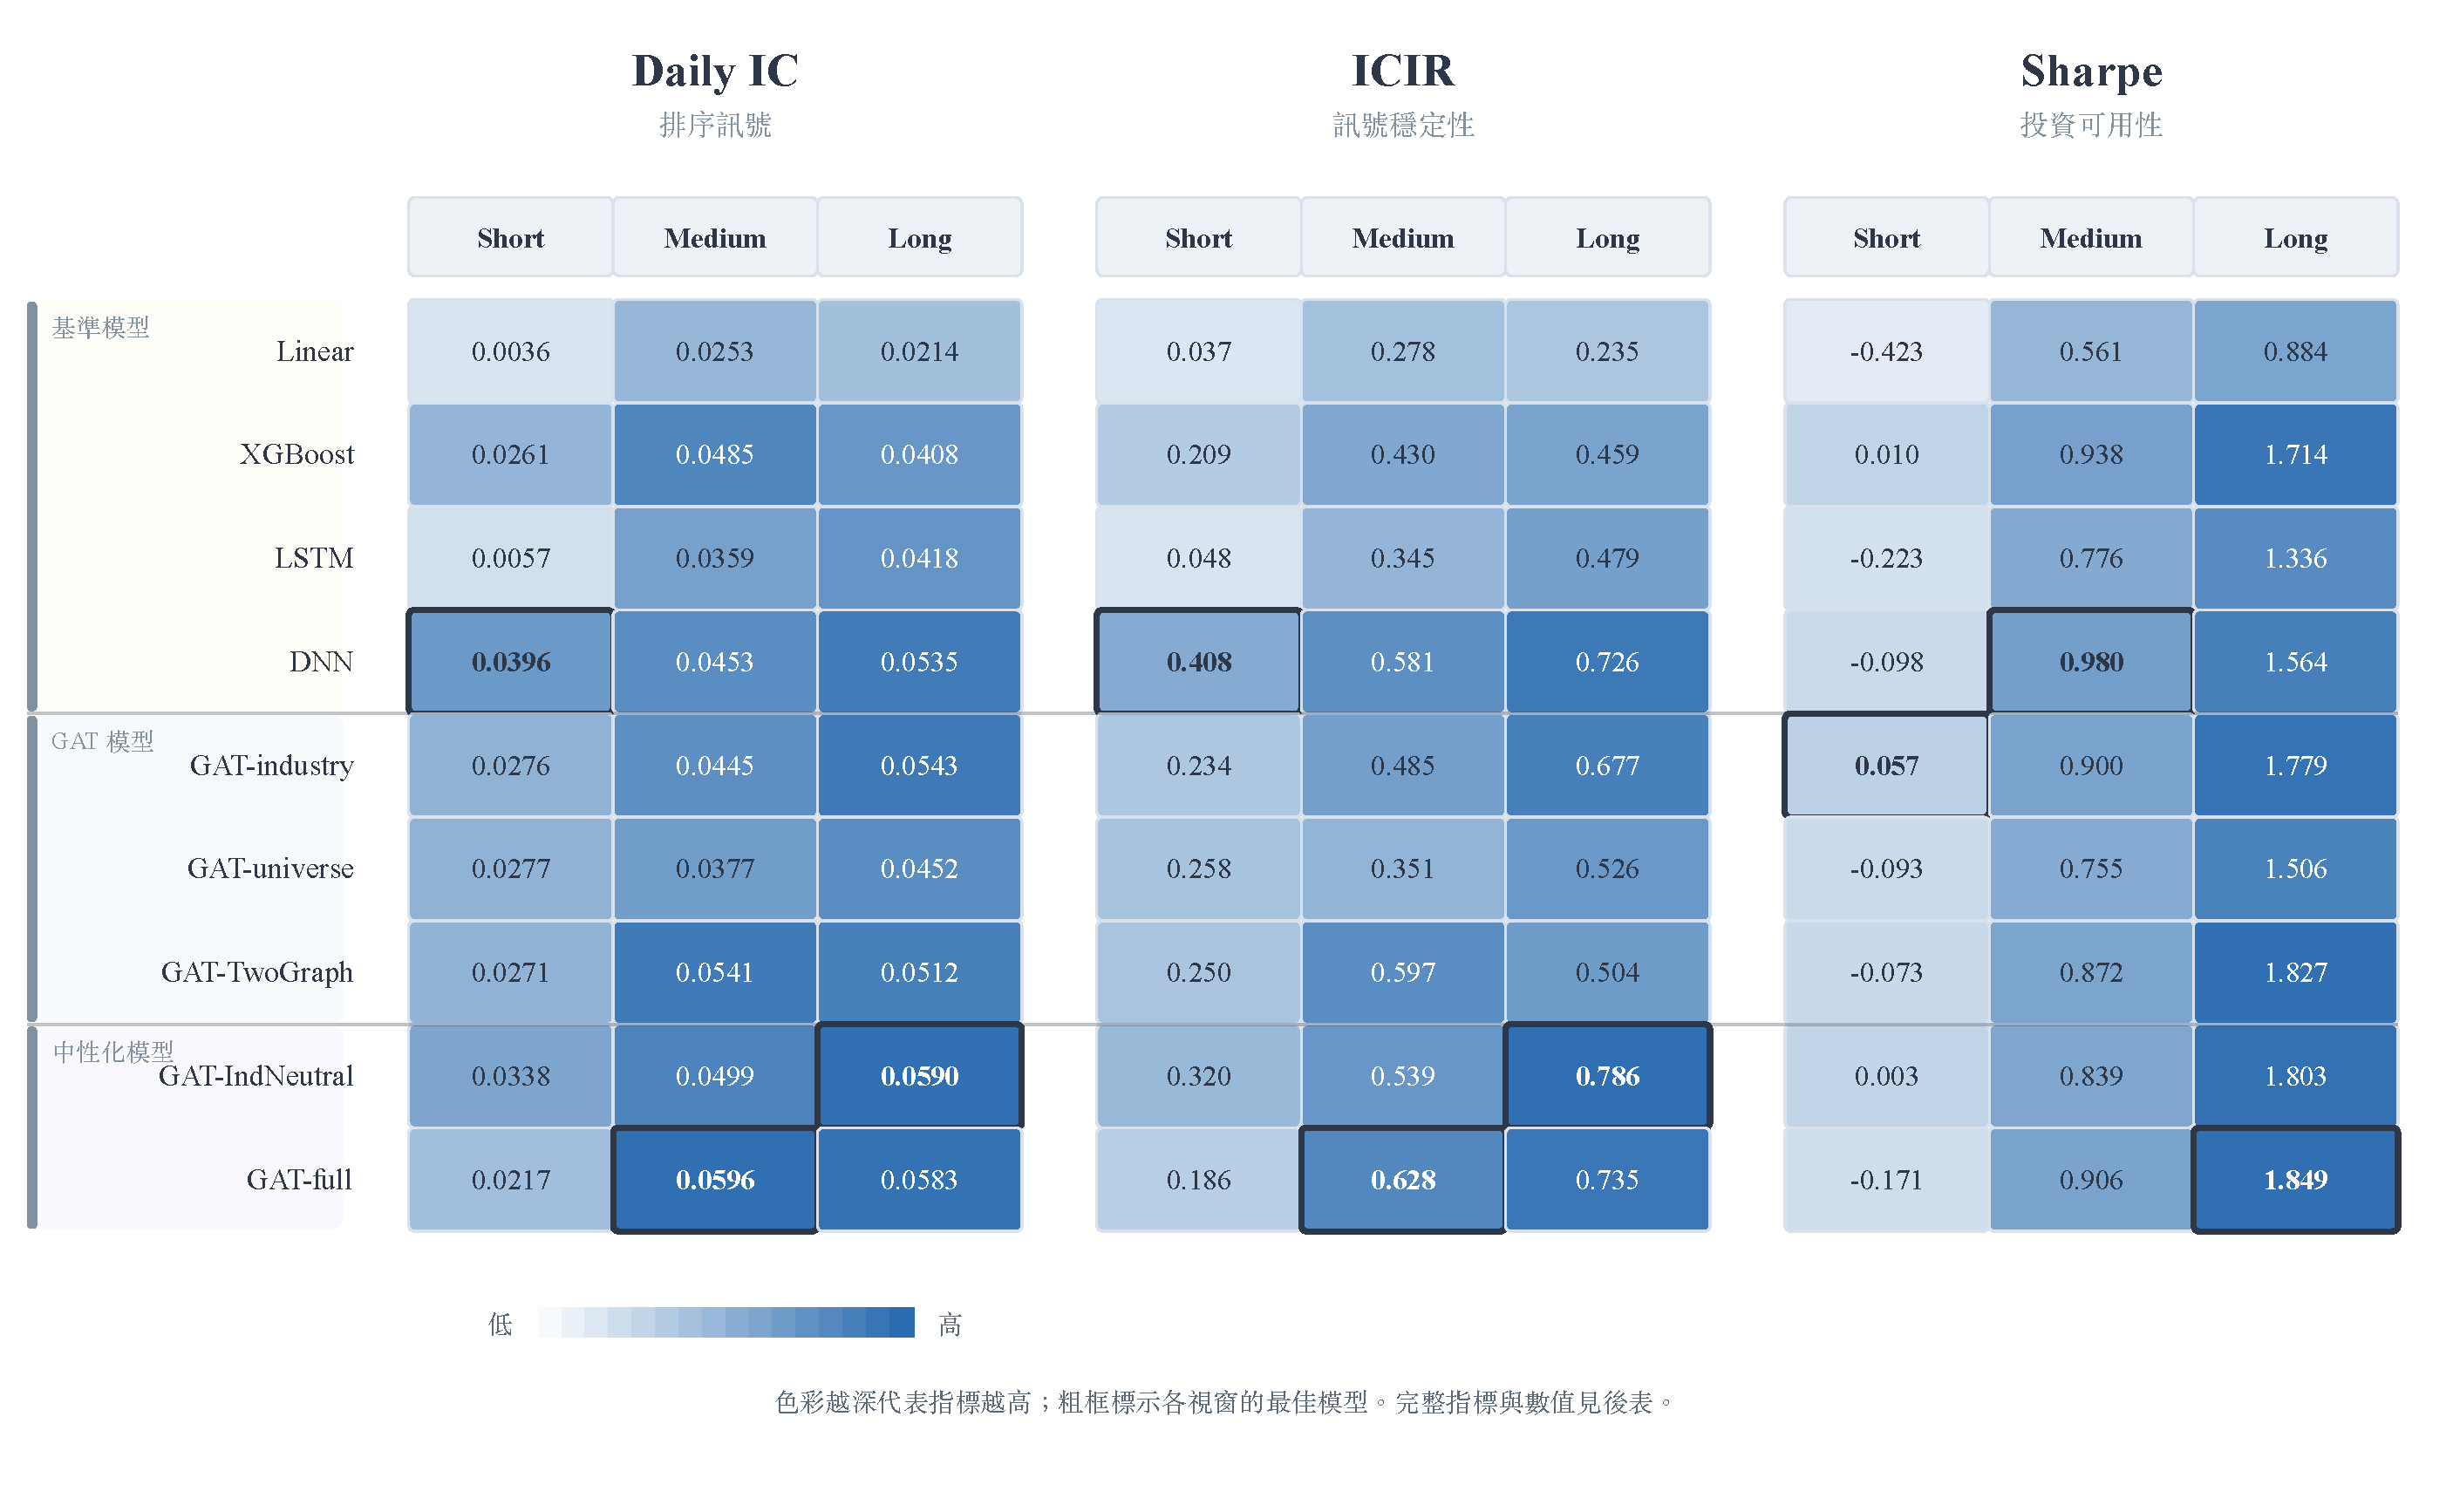
\includegraphics[width=\textwidth]{img/appendix_static_gpu_key_metrics_by_window.pdf}
  \caption{全模型核心指標之跨視窗比較}
  \label{fig:appendix_static_gpu_key_metrics_by_window}
\end{figure}

\begingroup
\small
\setlength{\tabcolsep}{3pt}
\begin{longtable}{llrrrrrr}
\caption{正式實驗全模型關鍵指標彙整（測試集）}
\label{tab:appendix_unified_key_metrics}\\
\toprule
時間窗 & 模型 & Test IC & Daily IC & ICIR & DirAcc & 總報酬 & Sharpe \\
\midrule
\endfirsthead
\toprule
時間窗 & 模型 & Test IC & Daily IC & ICIR & DirAcc & 總報酬 & Sharpe \\
\midrule
\endhead
\midrule
\multicolumn{8}{r}{（續下頁）}\\
\endfoot
\bottomrule
\endlastfoot
Short & Linear & 0.0050 & 0.0036 & 0.037 & 51.13\% & -11.26\% & -0.423 \\
Short & XGBoost & 0.0232 & 0.0261 & 0.209 & 52.18\% & -4.32\% & 0.010 \\
Short & LSTM & 0.0073 & 0.0057 & 0.048 & 49.57\% & -8.23\% & -0.223 \\
Short & DNN & 0.0363 & 0.0396 & 0.408 & 45.23\% & -5.88\% & -0.098 \\
Short & GAT-industry & 0.0267 & 0.0276 & 0.234 & 45.13\% & -3.23\% & 0.057 \\
Short & GAT-universe & 0.0287 & 0.0277 & 0.258 & 54.85\% & -6.13\% & -0.093 \\
Short & GAT-TwoGraph & 0.0267 & 0.0271 & 0.250 & 45.22\% & -5.77\% & -0.073 \\
Short & GAT-IndNeutral & 0.0324 & 0.0338 & 0.320 & 45.20\% & -3.85\% & 0.003 \\
Short & GAT-full & 0.0211 & 0.0217 & 0.186 & 45.85\% & -7.86\% & -0.171 \\
Medium & Linear & 0.0291 & 0.0253 & 0.278 & 51.32\% & 17.35\% & 0.561 \\
Medium & XGBoost & 0.0569 & 0.0485 & 0.430 & 51.13\% & 38.44\% & 0.938 \\
Medium & LSTM & 0.0406 & 0.0359 & 0.345 & 50.83\% & 29.16\% & 0.776 \\
Medium & DNN & 0.0472 & 0.0453 & 0.581 & 43.95\% & 39.13\% & 0.980 \\
Medium & GAT-industry & 0.0485 & 0.0445 & 0.485 & 56.91\% & 36.79\% & 0.900 \\
Medium & GAT-universe & 0.0474 & 0.0377 & 0.351 & 46.76\% & 28.88\% & 0.755 \\
Medium & GAT-TwoGraph & 0.0577 & 0.0541 & 0.597 & 56.88\% & 34.31\% & 0.872 \\
Medium & GAT-IndNeutral & 0.0511 & 0.0499 & 0.539 & 43.16\% & 33.04\% & 0.839 \\
Medium & GAT-full & 0.0631 & 0.0596 & 0.628 & 43.31\% & 36.29\% & 0.906 \\
Long & Linear & 0.0260 & 0.0214 & 0.235 & 51.46\% & 52.55\% & 0.884 \\
Long & XGBoost & 0.0205 & 0.0408 & 0.459 & 50.12\% & 143.08\% & 1.714 \\
Long & LSTM & 0.0438 & 0.0418 & 0.479 & 50.48\% & 95.50\% & 1.336 \\
Long & DNN & 0.0542 & 0.0535 & 0.726 & 42.58\% & 106.45\% & 1.564 \\
Long & GAT-industry & 0.0548 & 0.0543 & 0.677 & 57.51\% & 120.83\% & 1.779 \\
Long & GAT-universe & 0.0466 & 0.0452 & 0.526 & 42.93\% & 108.10\% & 1.506 \\
Long & GAT-TwoGraph & 0.0520 & 0.0512 & 0.504 & 57.50\% & 127.33\% & 1.827 \\
Long & GAT-IndNeutral & 0.0591 & 0.0590 & 0.786 & 57.51\% & 123.60\% & 1.803 \\
Long & GAT-full & 0.0602 & 0.0583 & 0.735 & 57.52\% & 139.08\% & 1.849 \\
\end{longtable}
\endgroup


\clearpage
\subsection{完整累積報酬圖}

\begin{figure}[H]
  \centering
  \captionsetup[subfigure]{font=small}
  \begin{subfigure}[t]{0.47\textwidth}
    \centering
    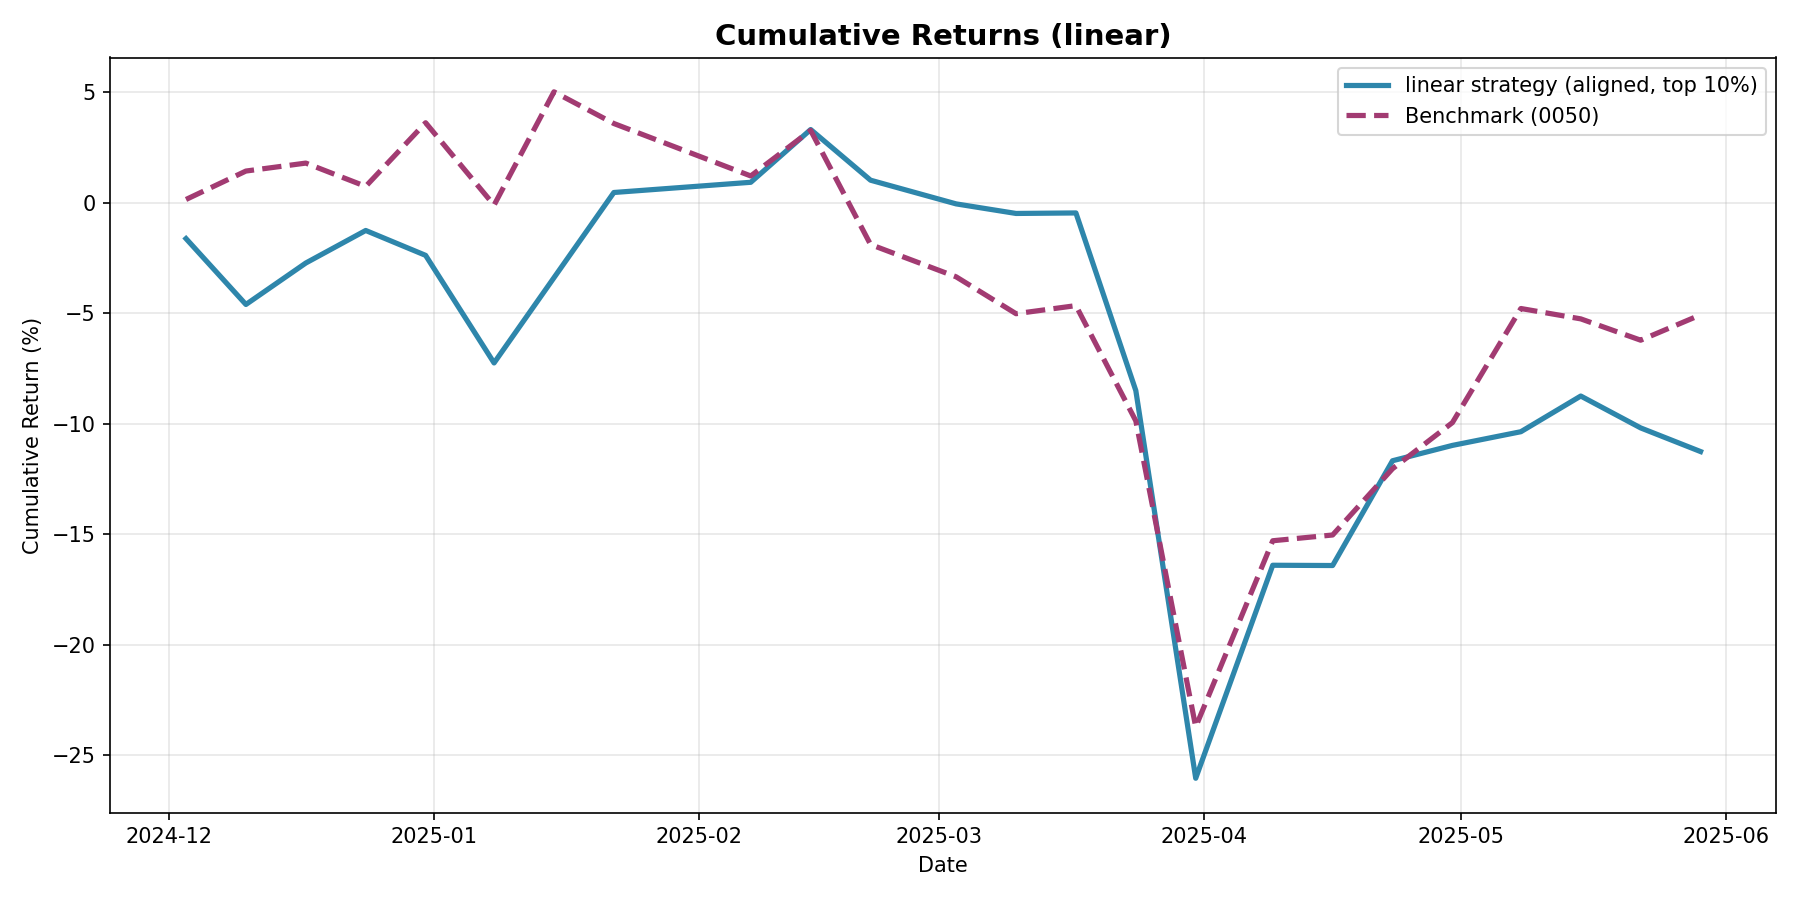
\includegraphics[width=\textwidth]{runs_gpu_static_to_20250601/static/short/baseline_linear/plots/cum_returns.png}
    \caption{Linear}
  \end{subfigure}
  \hfill
  \begin{subfigure}[t]{0.47\textwidth}
    \centering
    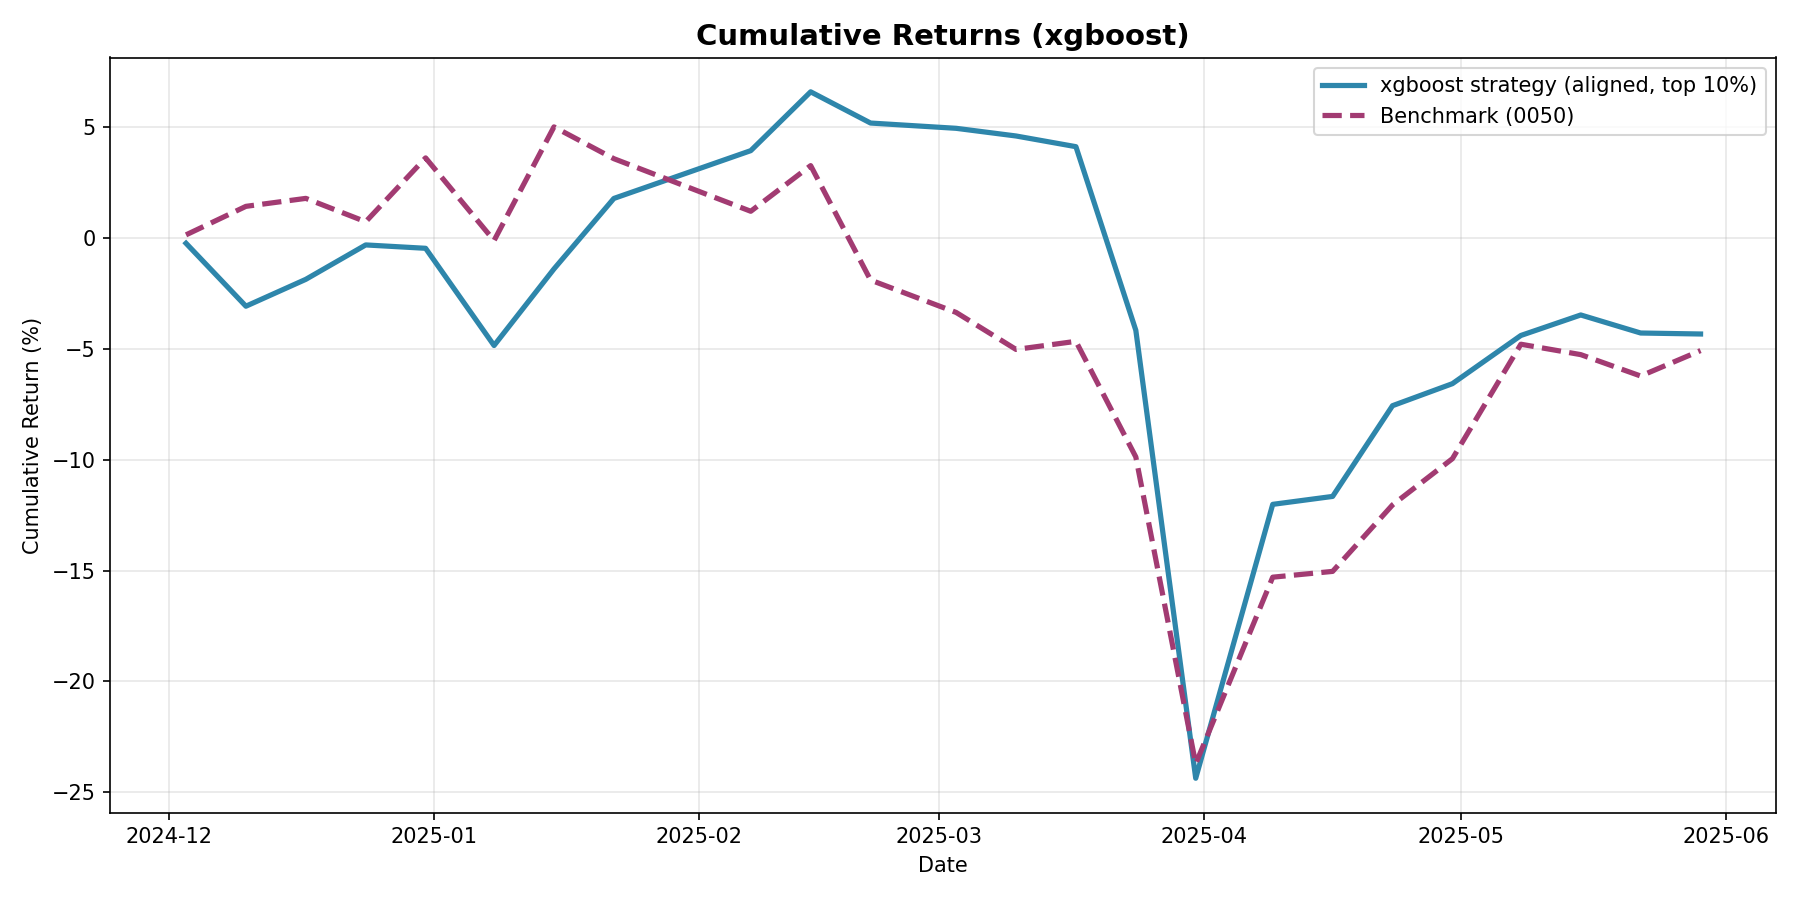
\includegraphics[width=\textwidth]{runs_gpu_static_to_20250601/static/short/baseline_xgboost/plots/cum_returns.png}
    \caption{XGBoost}
  \end{subfigure}
  \par\vspace{0.5em}
  \begin{subfigure}[t]{0.47\textwidth}
    \centering
    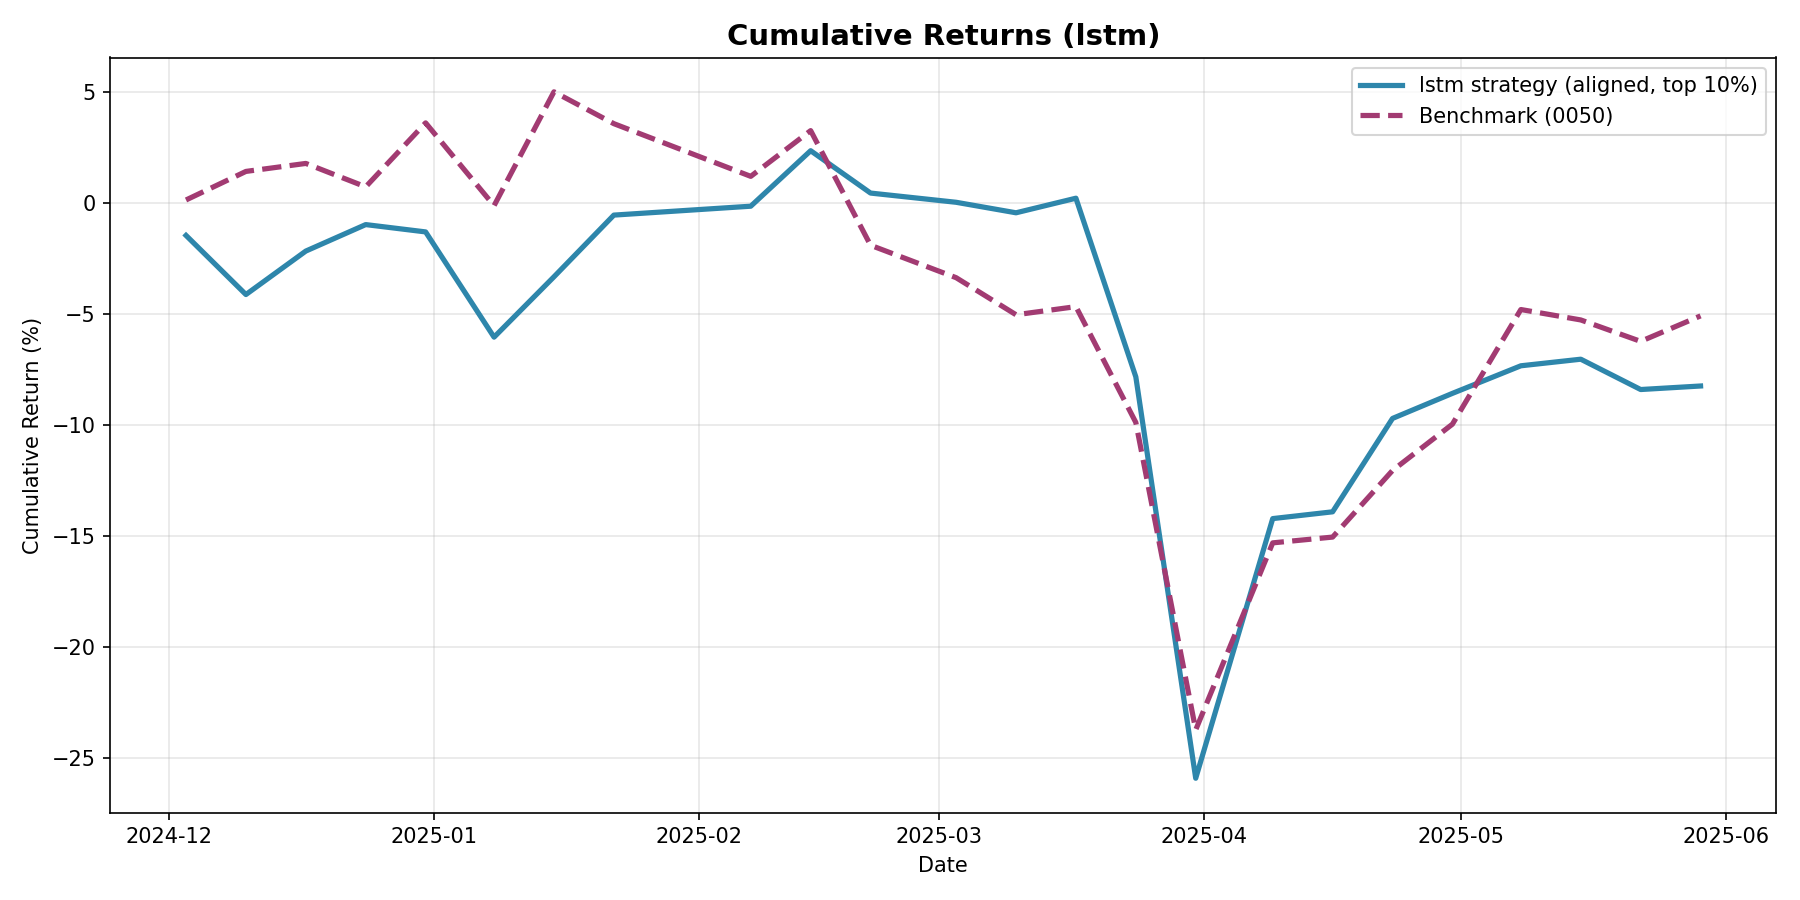
\includegraphics[width=\textwidth]{runs_gpu_static_to_20250601/static/short/baseline_lstm/plots/cum_returns.png}
    \caption{LSTM}
  \end{subfigure}
  \hfill
  \begin{subfigure}[t]{0.47\textwidth}
    \centering
    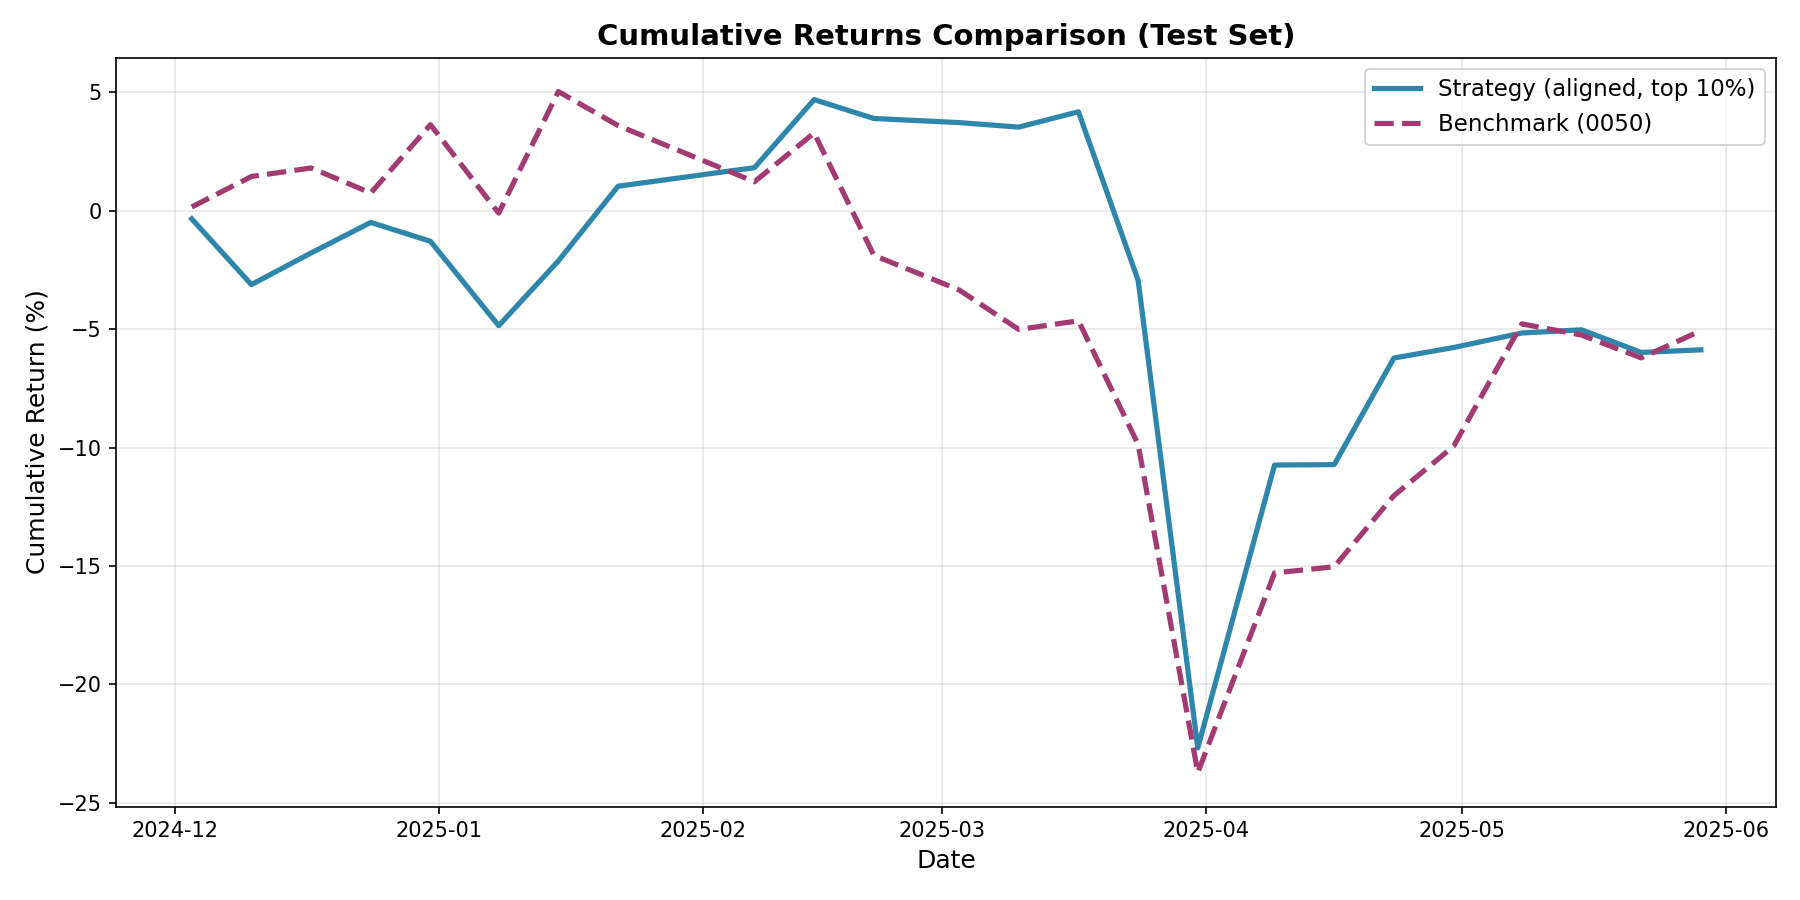
\includegraphics[width=\textwidth]{runs_gpu_static_to_20250601/static/short/mlp/plots/cum_returns.png}
    \caption{DNN}
  \end{subfigure}
  \par\vspace{0.5em}
  \begin{subfigure}[t]{0.47\textwidth}
    \centering
    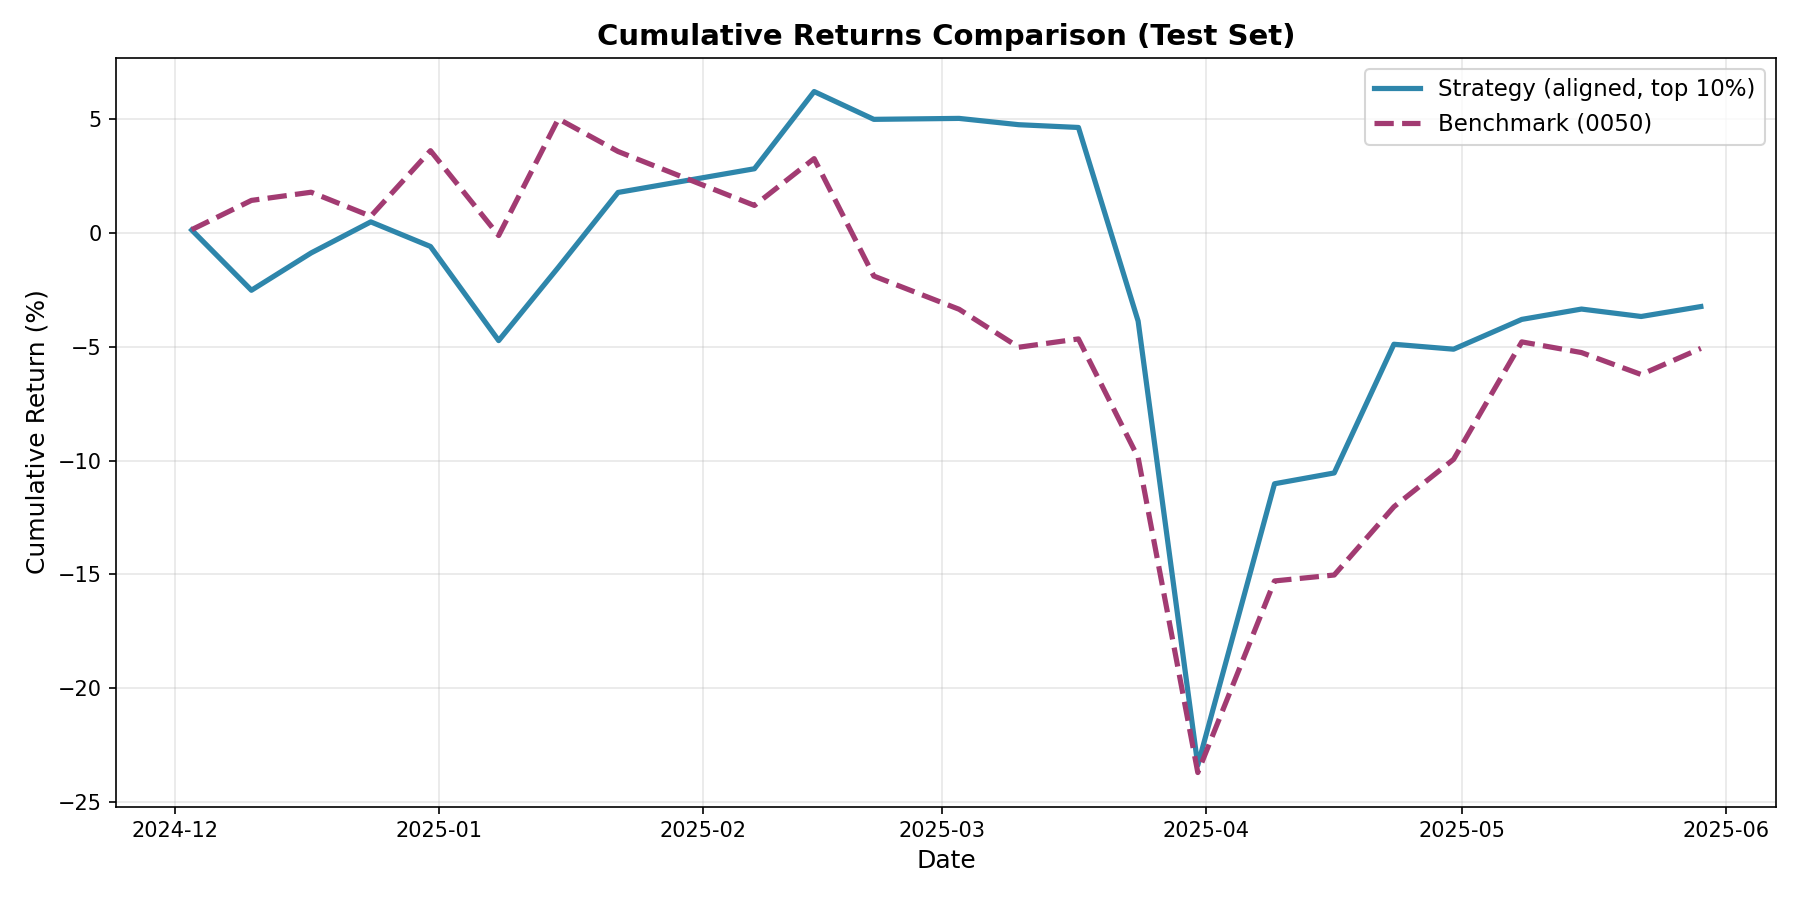
\includegraphics[width=\textwidth]{runs_gpu_static_to_20250601/static/short/gat_industry/plots/cum_returns.png}
    \caption{GAT-industry}
  \end{subfigure}
  \hfill
  \begin{subfigure}[t]{0.47\textwidth}
    \centering
    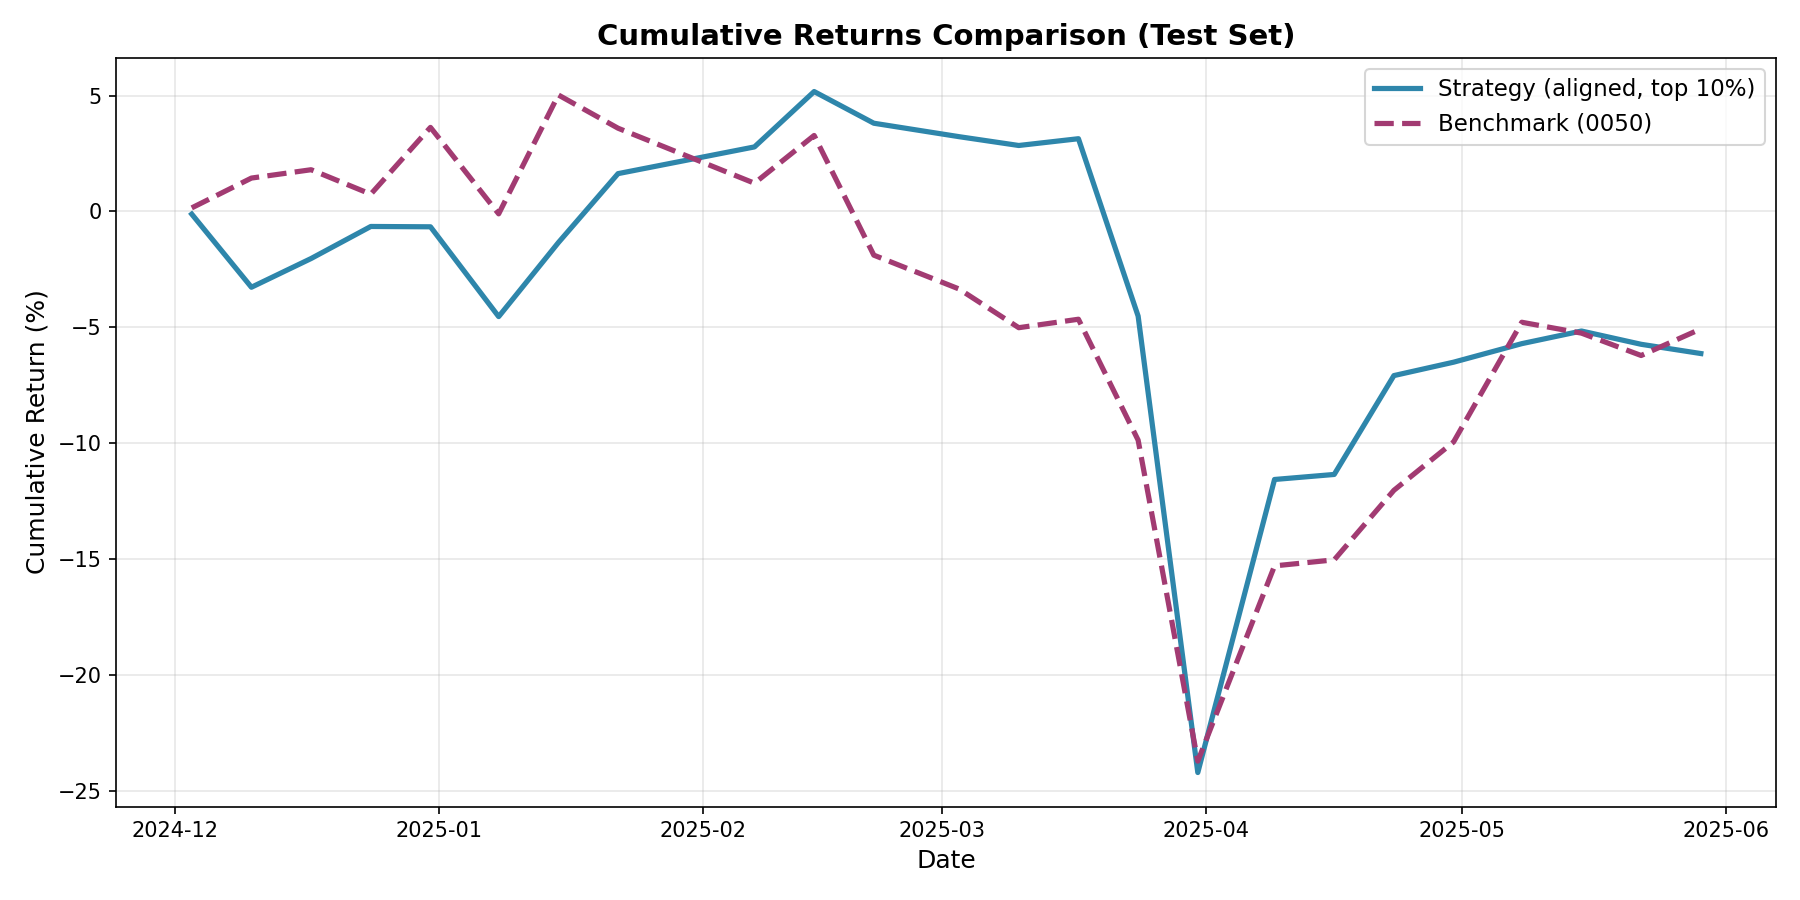
\includegraphics[width=\textwidth]{runs_gpu_static_to_20250601/static/short/gat_universe/plots/cum_returns.png}
    \caption{GAT-universe}
  \end{subfigure}
  \par\vspace{0.5em}
  \begin{subfigure}[t]{0.47\textwidth}
    \centering
    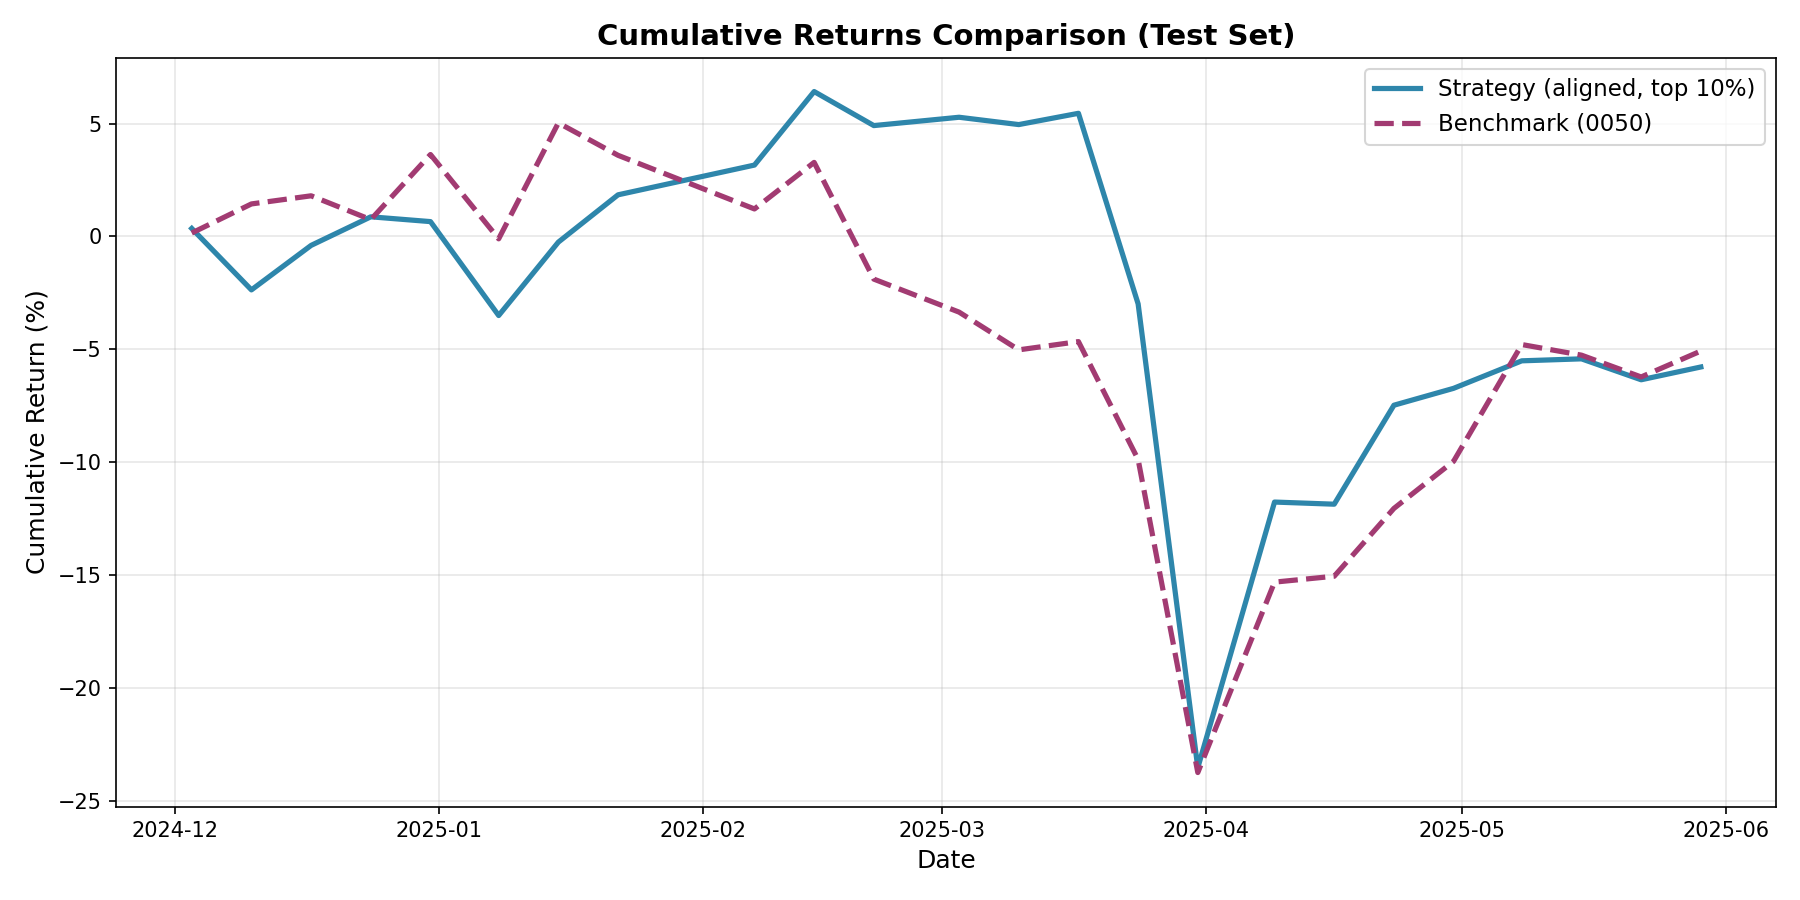
\includegraphics[width=\textwidth]{runs_gpu_static_to_20250601/static/short/gat_two_graph_no_neutral/plots/cum_returns.png}
    \caption{GAT-TwoGraph}
  \end{subfigure}
  \hfill
  \begin{subfigure}[t]{0.47\textwidth}
    \centering
    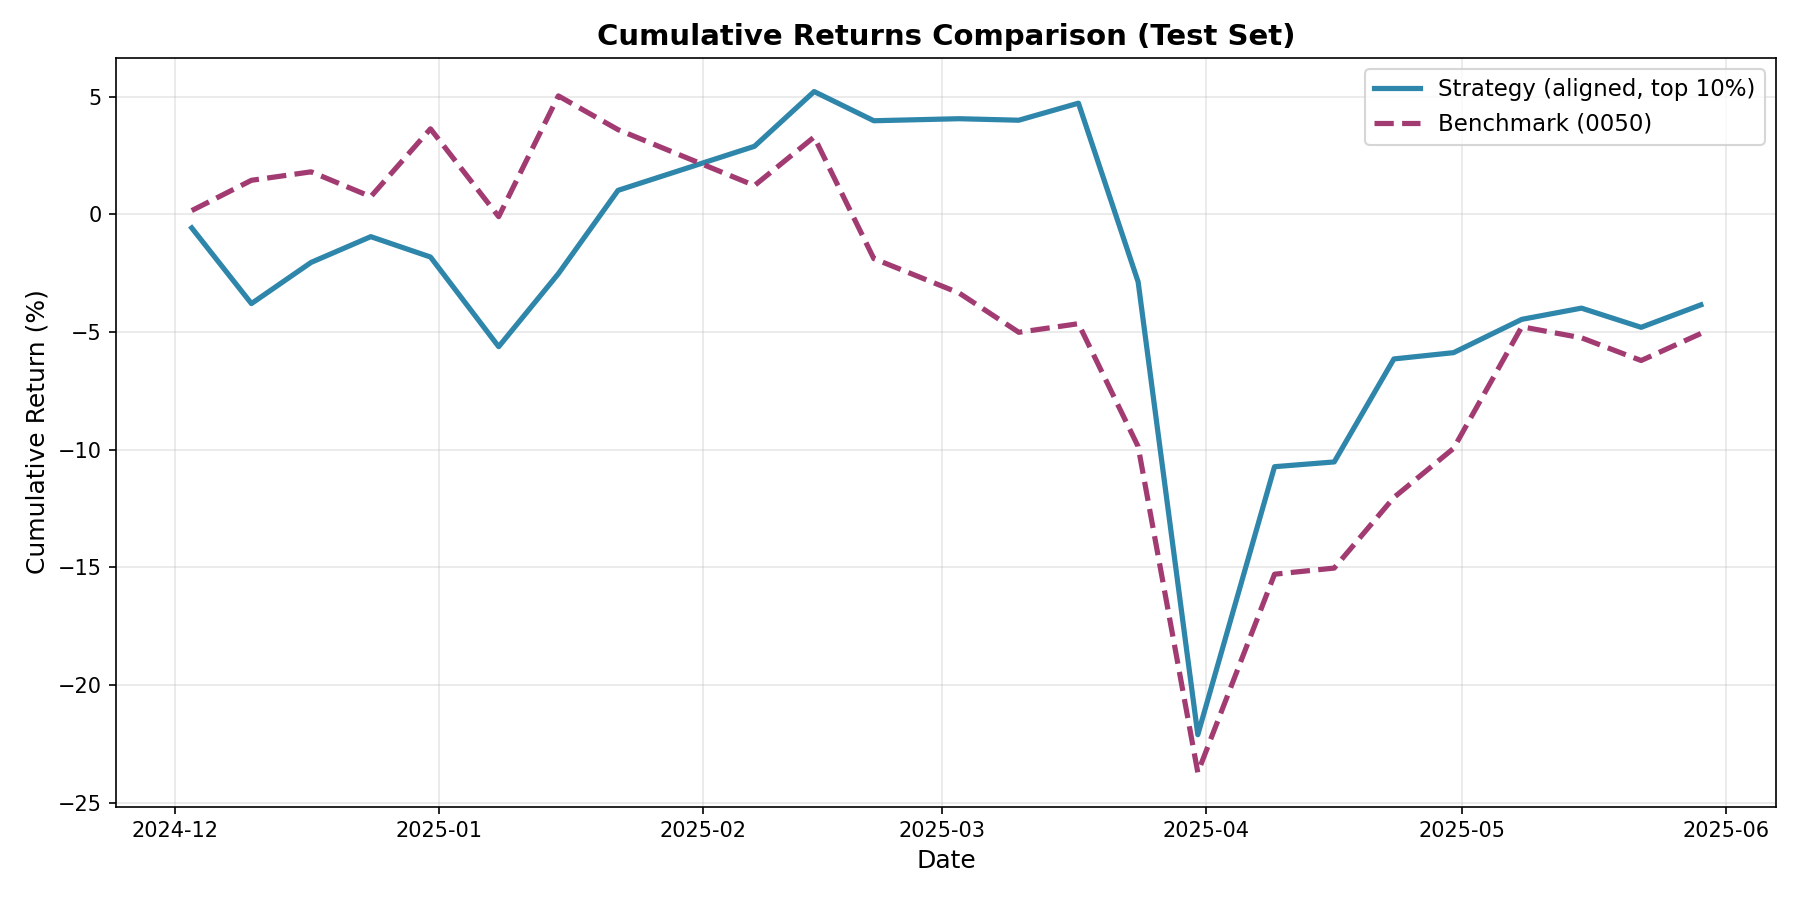
\includegraphics[width=\textwidth]{runs_gpu_static_to_20250601/static/short/dmfm_ind_neutral/plots/cum_returns.png}
    \caption{GAT-IndNeutral}
  \end{subfigure}
  \par\vspace{0.5em}
  \hfill
  \begin{subfigure}[t]{0.47\textwidth}
    \centering
    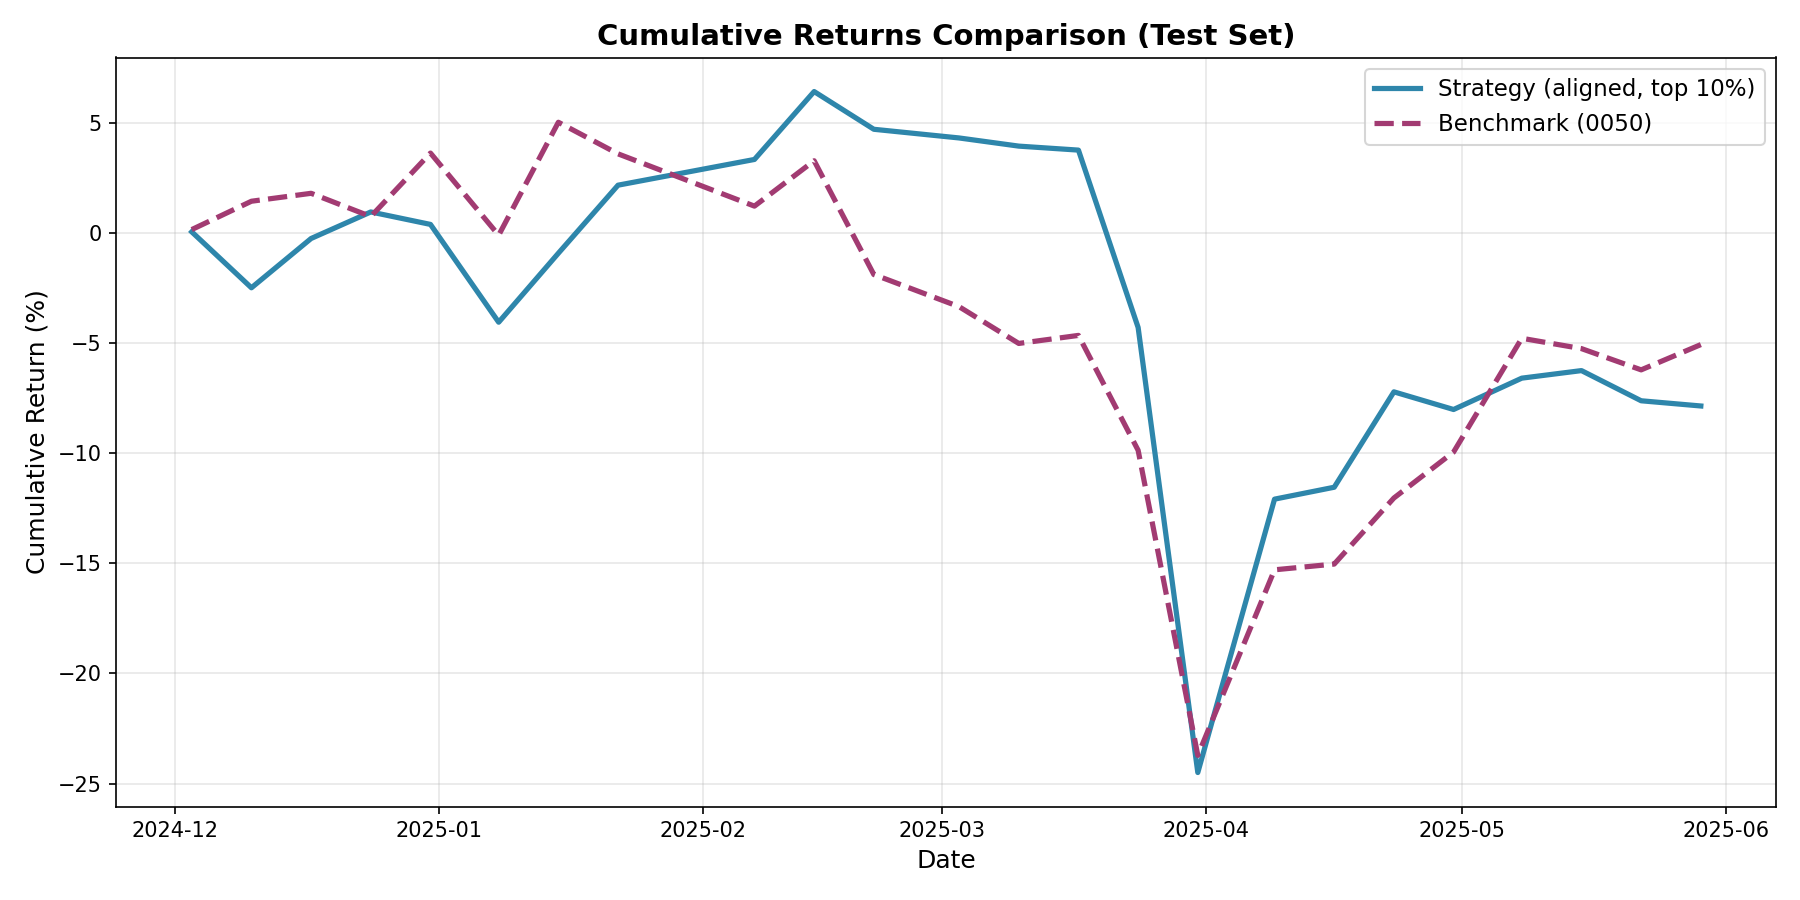
\includegraphics[width=\textwidth]{runs_gpu_static_to_20250601/static/short/dmfm_full/plots/cum_returns.png}
    \caption{GAT-full}
  \end{subfigure}
  \hfill
  \par\vspace{0.3em}
  \caption{Short window 各模型累積報酬曲線。}
  \label{fig:appendix_static_cum_returns_short}
\end{figure}

\clearpage
\begin{figure}[H]
  \centering
  \captionsetup[subfigure]{font=small}
  \begin{subfigure}[t]{0.47\textwidth}
    \centering
    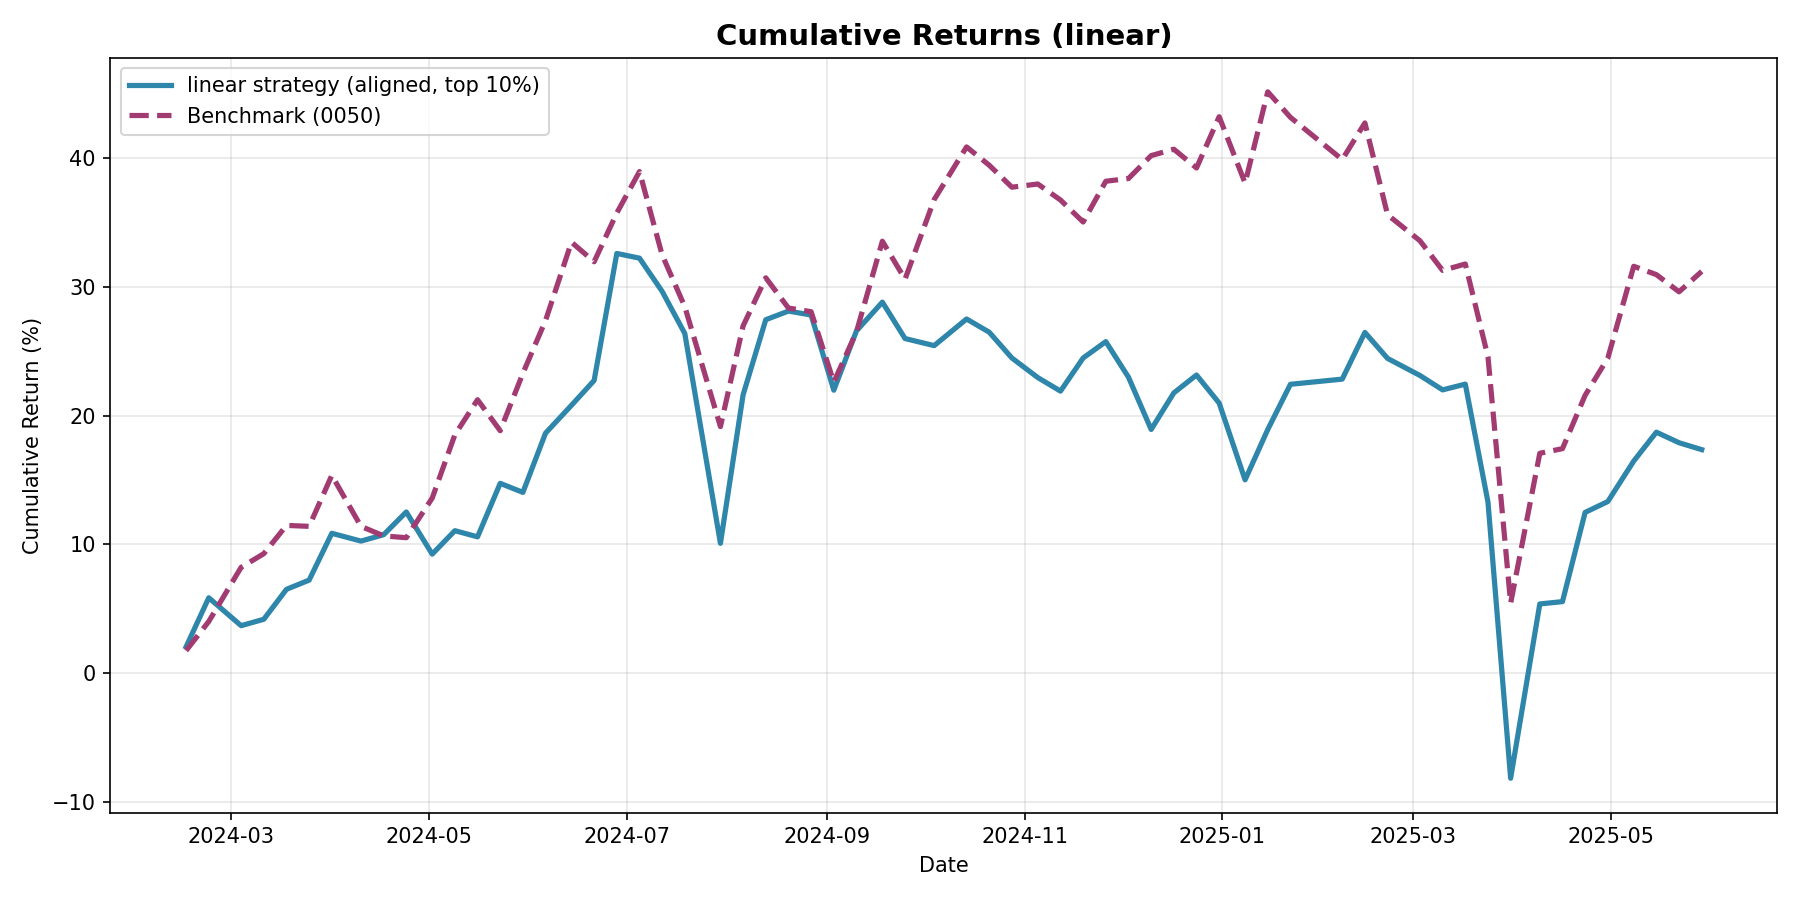
\includegraphics[width=\textwidth]{runs_gpu_static_to_20250601/static/medium/baseline_linear/plots/cum_returns.png}
    \caption{Linear}
  \end{subfigure}
  \hfill
  \begin{subfigure}[t]{0.47\textwidth}
    \centering
    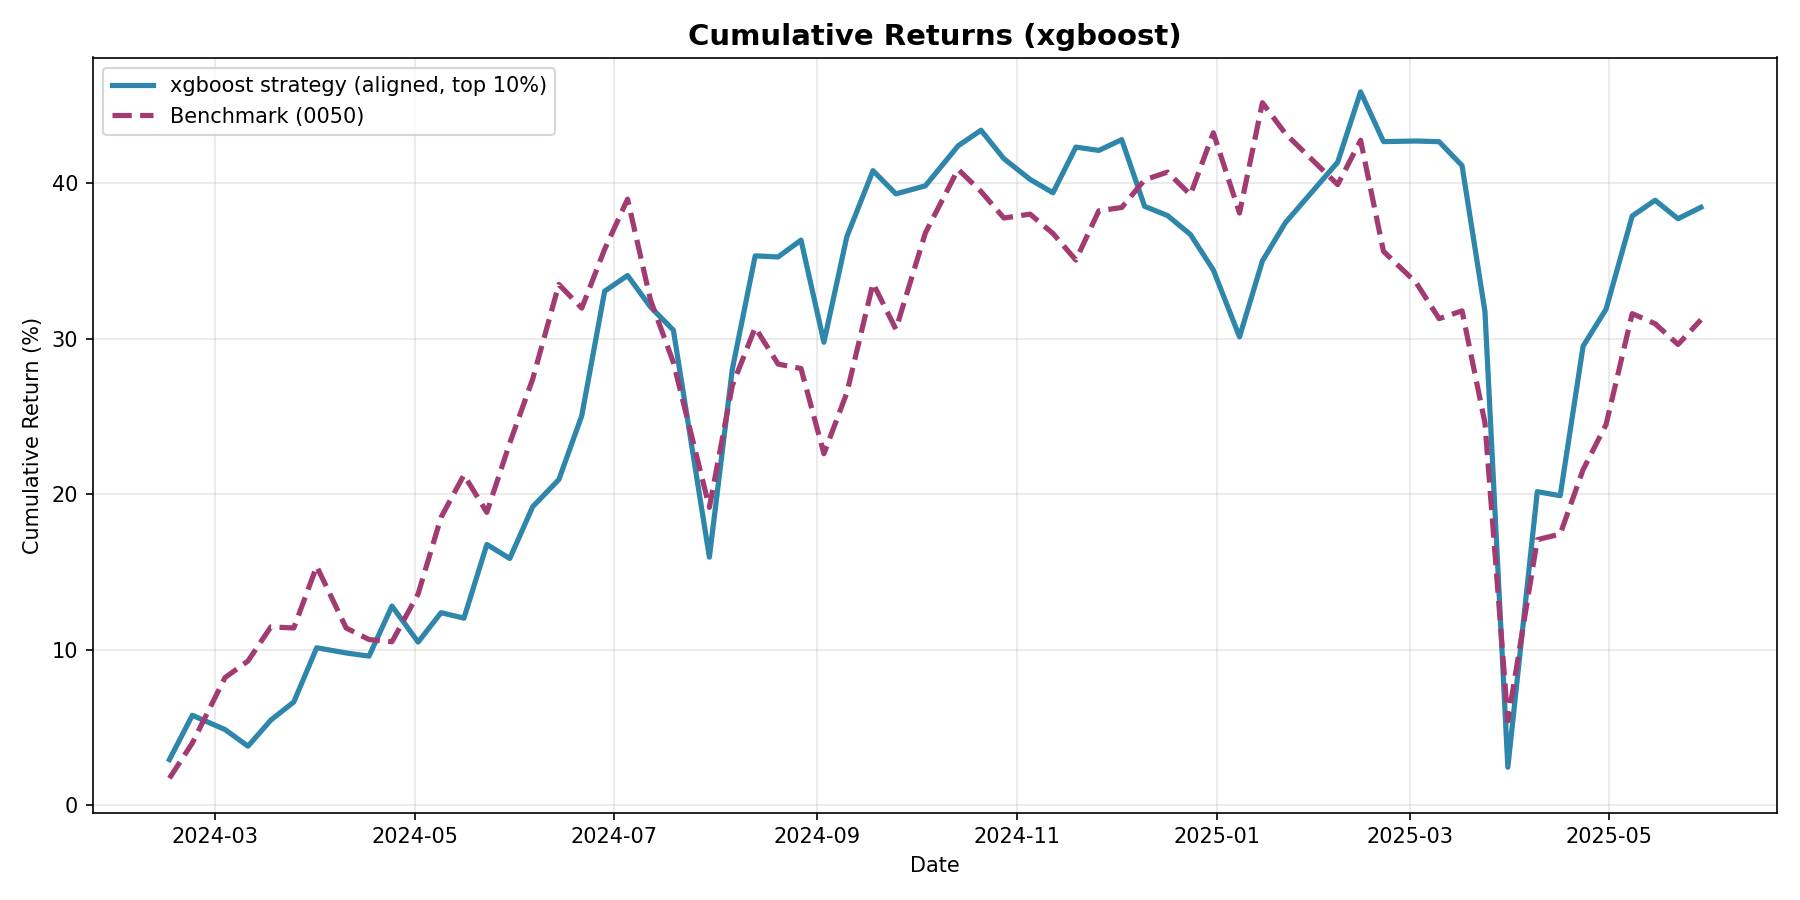
\includegraphics[width=\textwidth]{runs_gpu_static_to_20250601/static/medium/baseline_xgboost/plots/cum_returns.png}
    \caption{XGBoost}
  \end{subfigure}
  \par\vspace{0.5em}
  \begin{subfigure}[t]{0.47\textwidth}
    \centering
    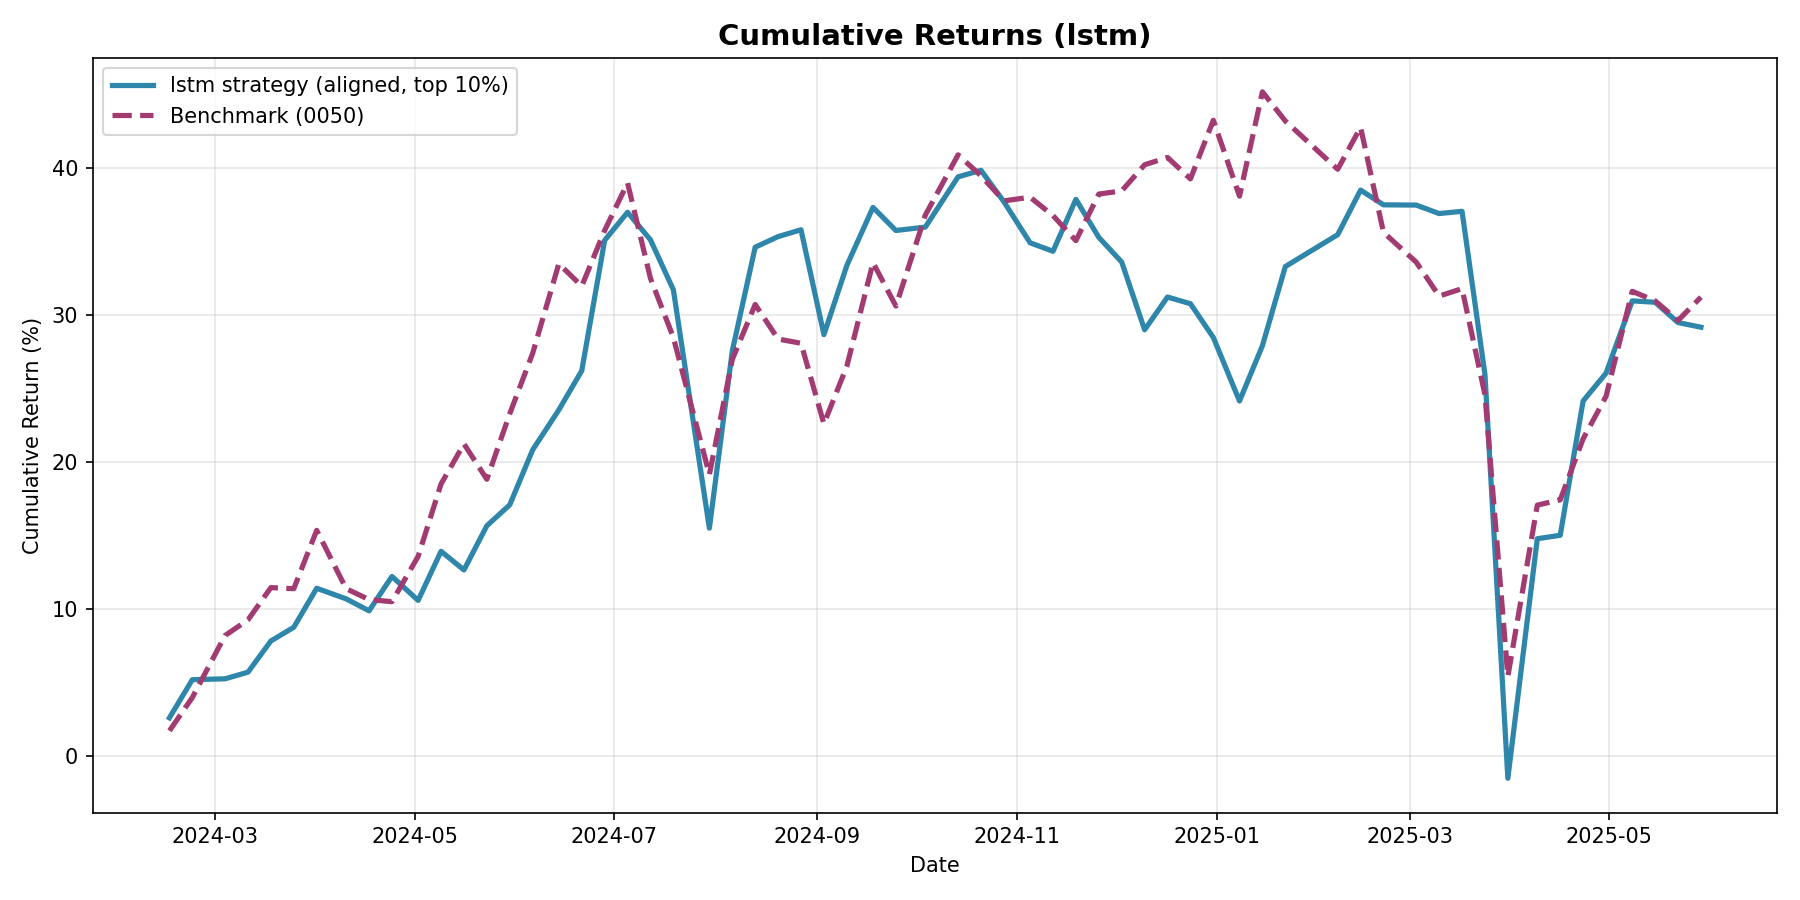
\includegraphics[width=\textwidth]{runs_gpu_static_to_20250601/static/medium/baseline_lstm/plots/cum_returns.png}
    \caption{LSTM}
  \end{subfigure}
  \hfill
  \begin{subfigure}[t]{0.47\textwidth}
    \centering
    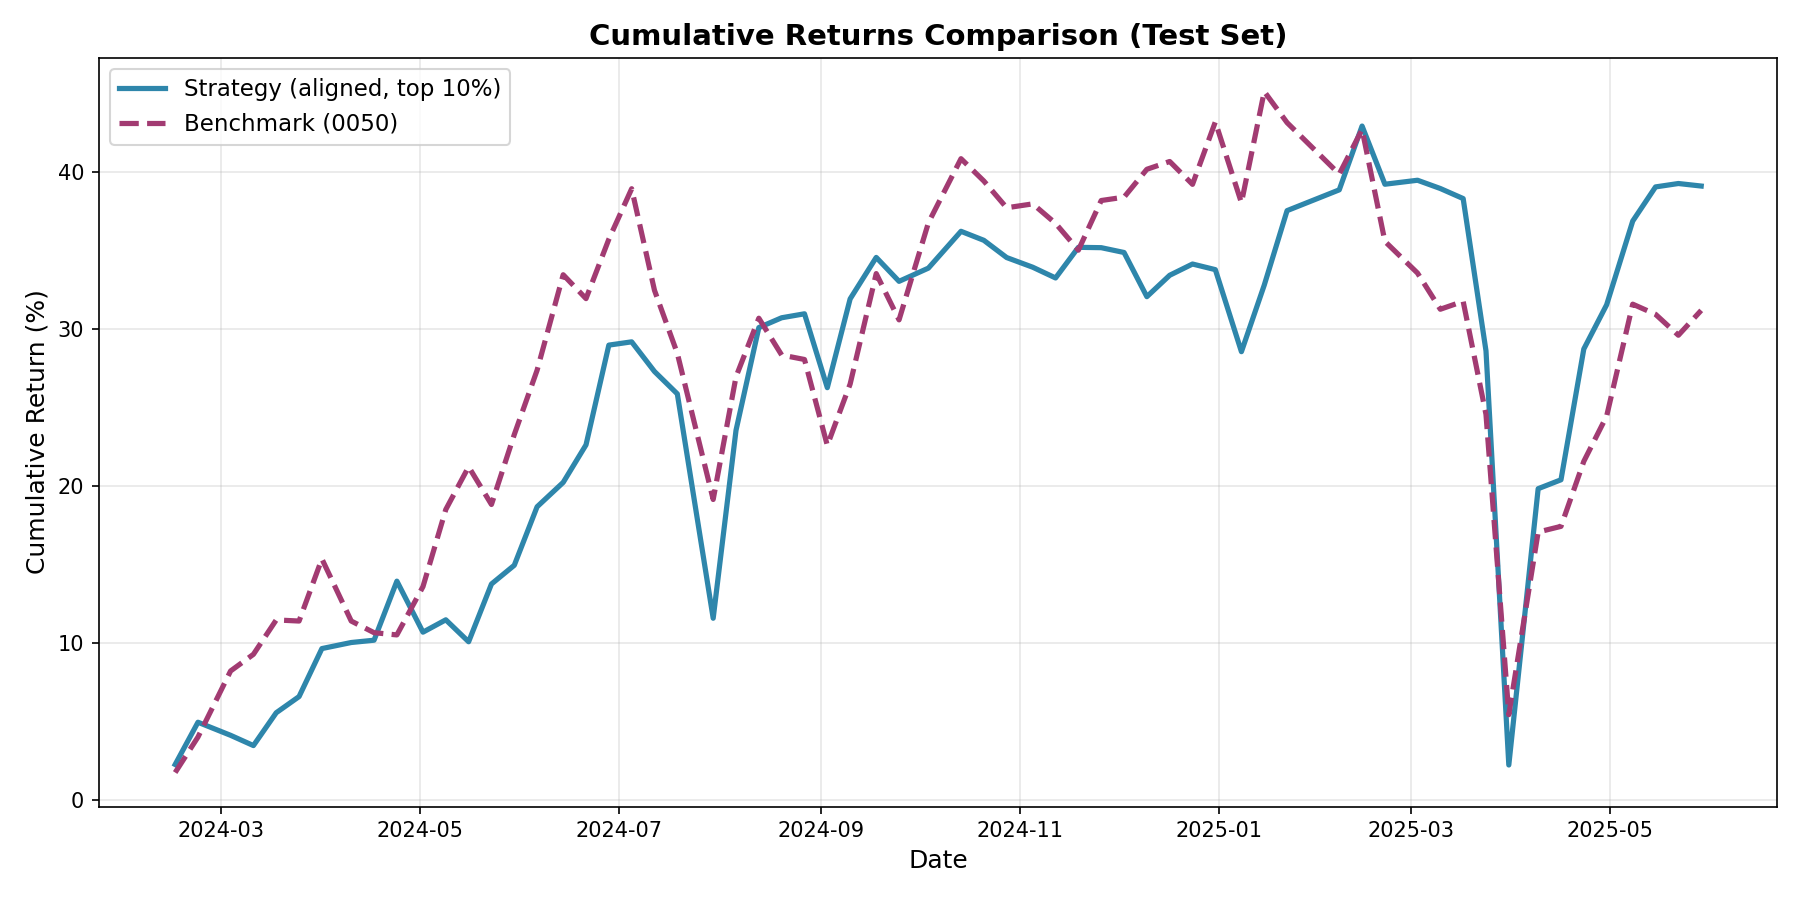
\includegraphics[width=\textwidth]{runs_gpu_static_to_20250601/static/medium/mlp/plots/cum_returns.png}
    \caption{DNN}
  \end{subfigure}
  \par\vspace{0.5em}
  \begin{subfigure}[t]{0.47\textwidth}
    \centering
    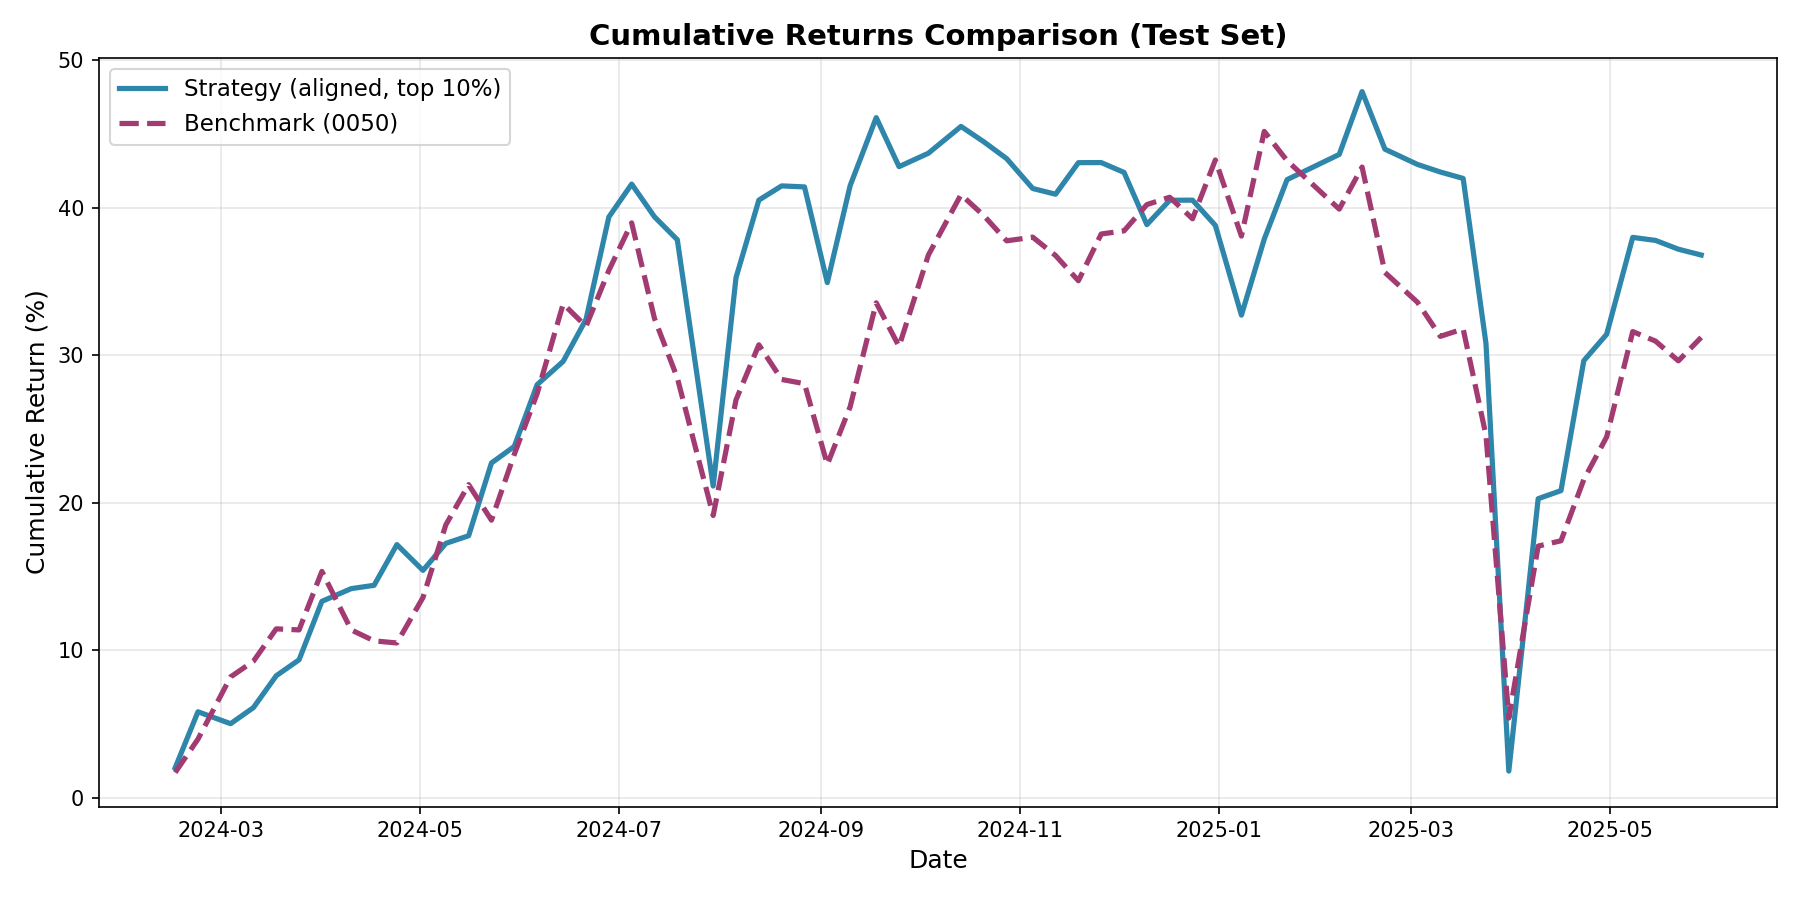
\includegraphics[width=\textwidth]{runs_gpu_static_to_20250601/static/medium/gat_industry/plots/cum_returns.png}
    \caption{GAT-industry}
  \end{subfigure}
  \hfill
  \begin{subfigure}[t]{0.47\textwidth}
    \centering
    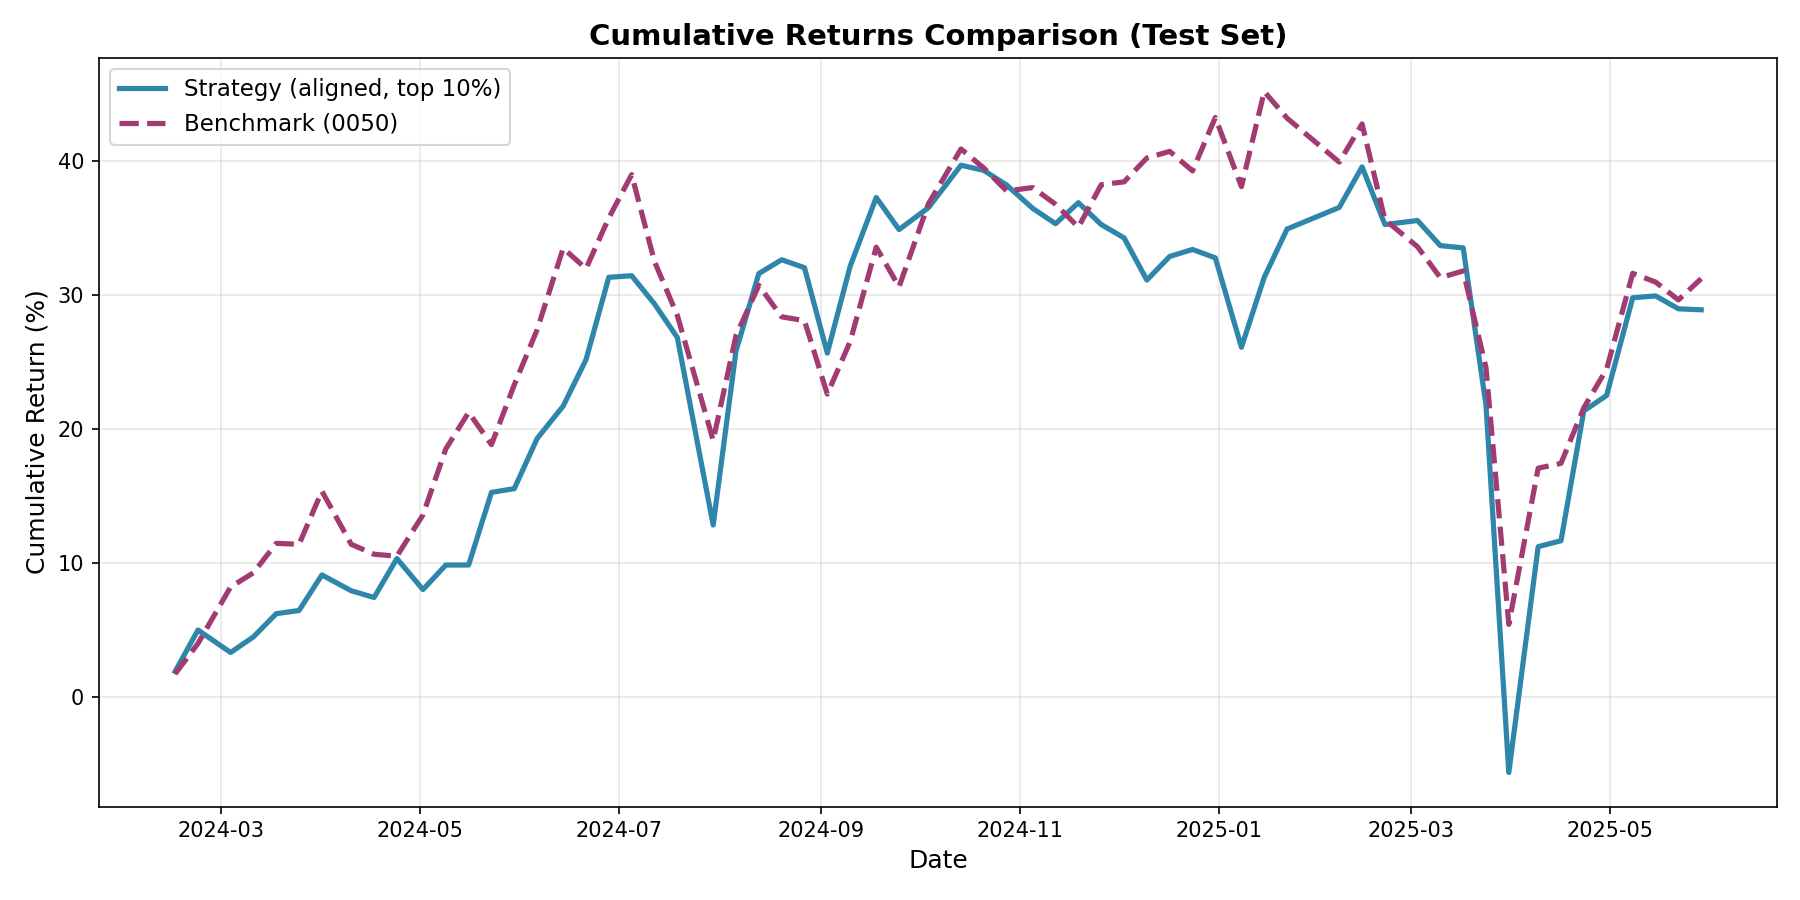
\includegraphics[width=\textwidth]{runs_gpu_static_to_20250601/static/medium/gat_universe/plots/cum_returns.png}
    \caption{GAT-universe}
  \end{subfigure}
  \par\vspace{0.5em}
  \begin{subfigure}[t]{0.47\textwidth}
    \centering
    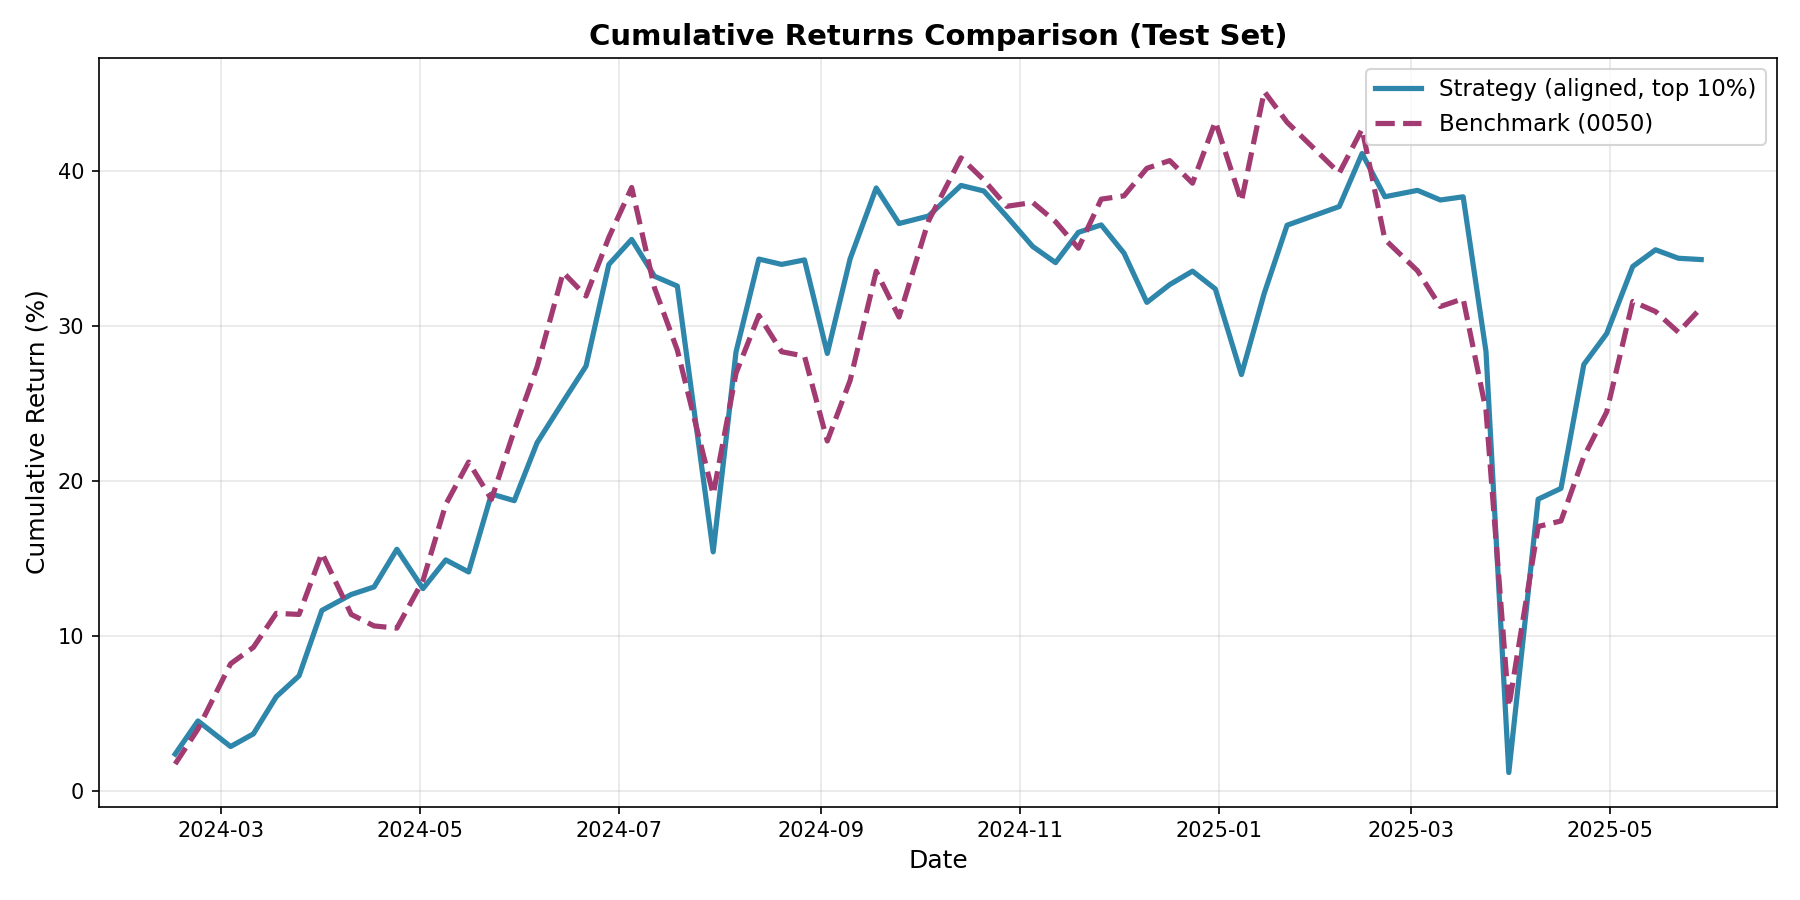
\includegraphics[width=\textwidth]{runs_gpu_static_to_20250601/static/medium/gat_two_graph_no_neutral/plots/cum_returns.png}
    \caption{GAT-TwoGraph}
  \end{subfigure}
  \hfill
  \begin{subfigure}[t]{0.47\textwidth}
    \centering
    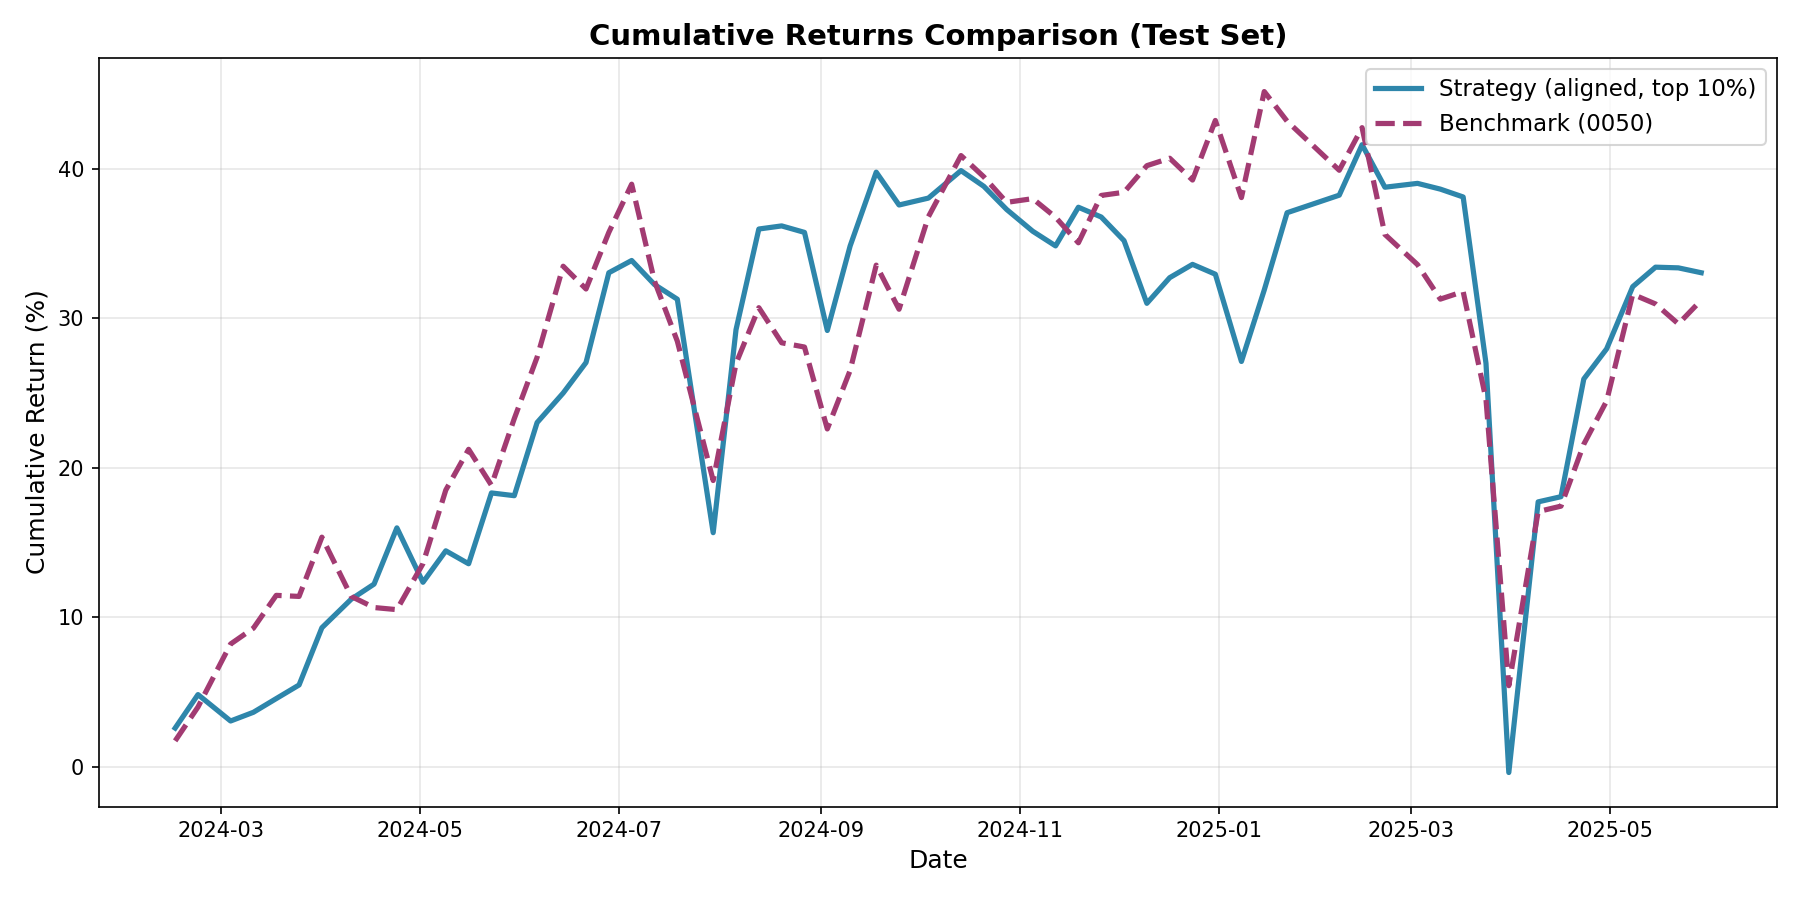
\includegraphics[width=\textwidth]{runs_gpu_static_to_20250601/static/medium/dmfm_ind_neutral/plots/cum_returns.png}
    \caption{GAT-IndNeutral}
  \end{subfigure}
  \par\vspace{0.5em}
  \hfill
  \begin{subfigure}[t]{0.47\textwidth}
    \centering
    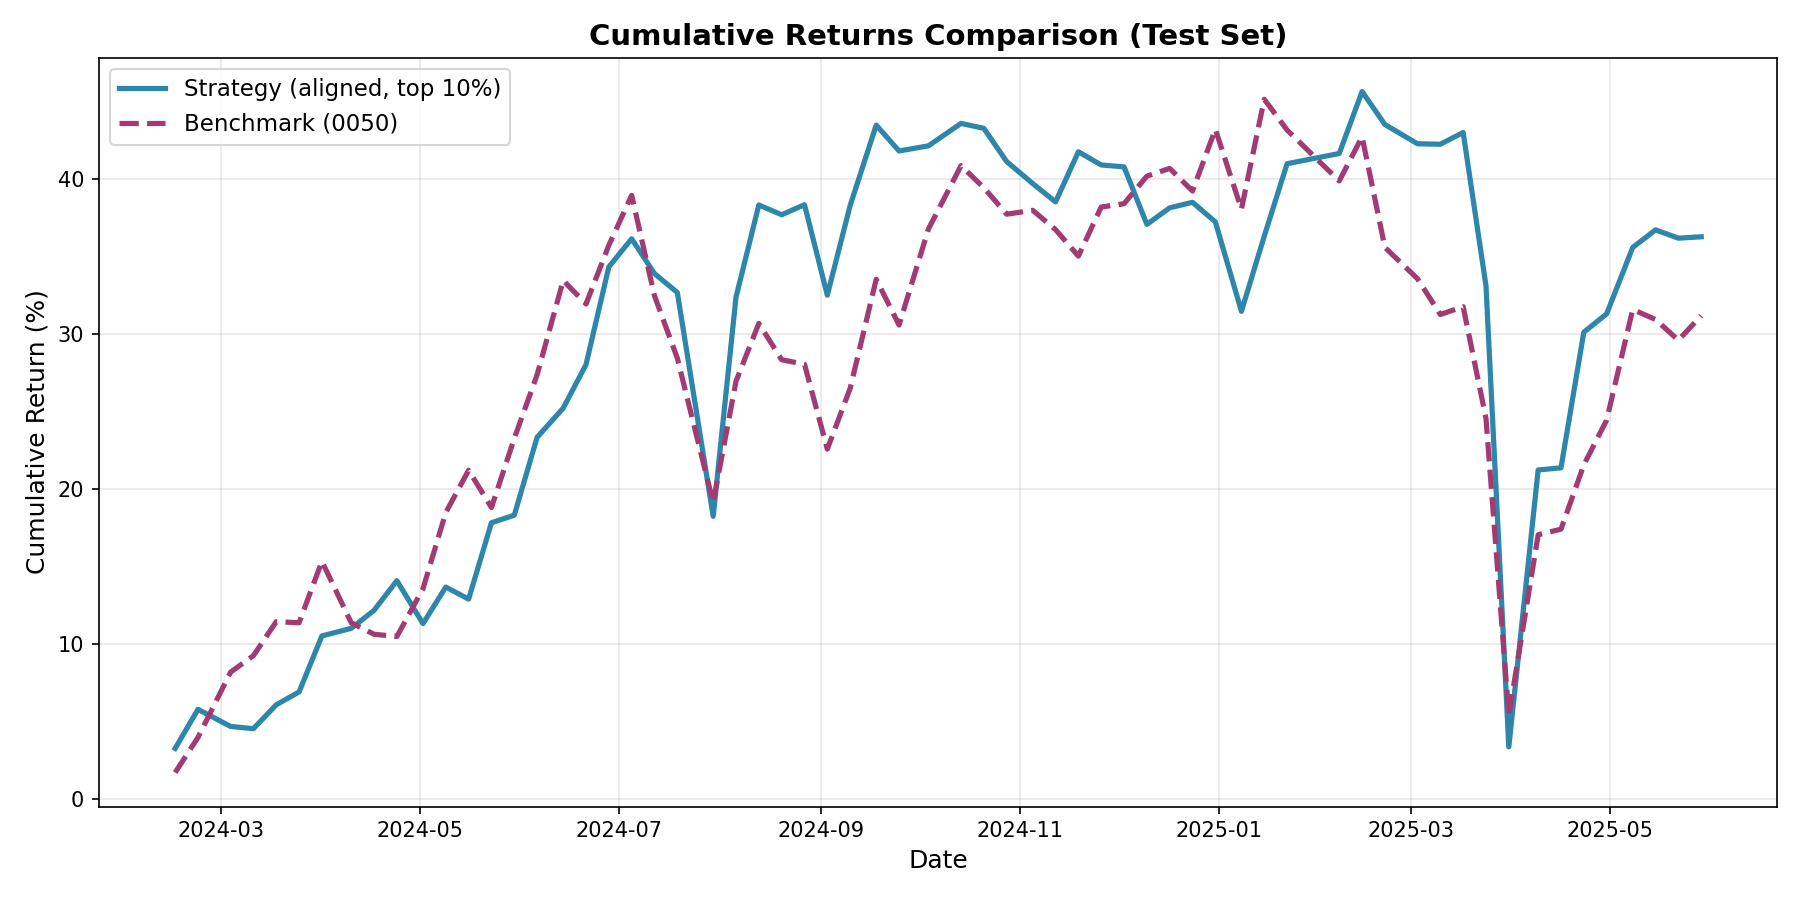
\includegraphics[width=\textwidth]{runs_gpu_static_to_20250601/static/medium/dmfm_full/plots/cum_returns.png}
    \caption{GAT-full}
  \end{subfigure}
  \hfill
  \par\vspace{0.3em}
  \caption{Medium window 各模型累積報酬曲線。}
  \label{fig:appendix_static_cum_returns_medium}
\end{figure}

\clearpage
\begin{figure}[H]
  \centering
  \captionsetup[subfigure]{font=small}
  \begin{subfigure}[t]{0.47\textwidth}
    \centering
    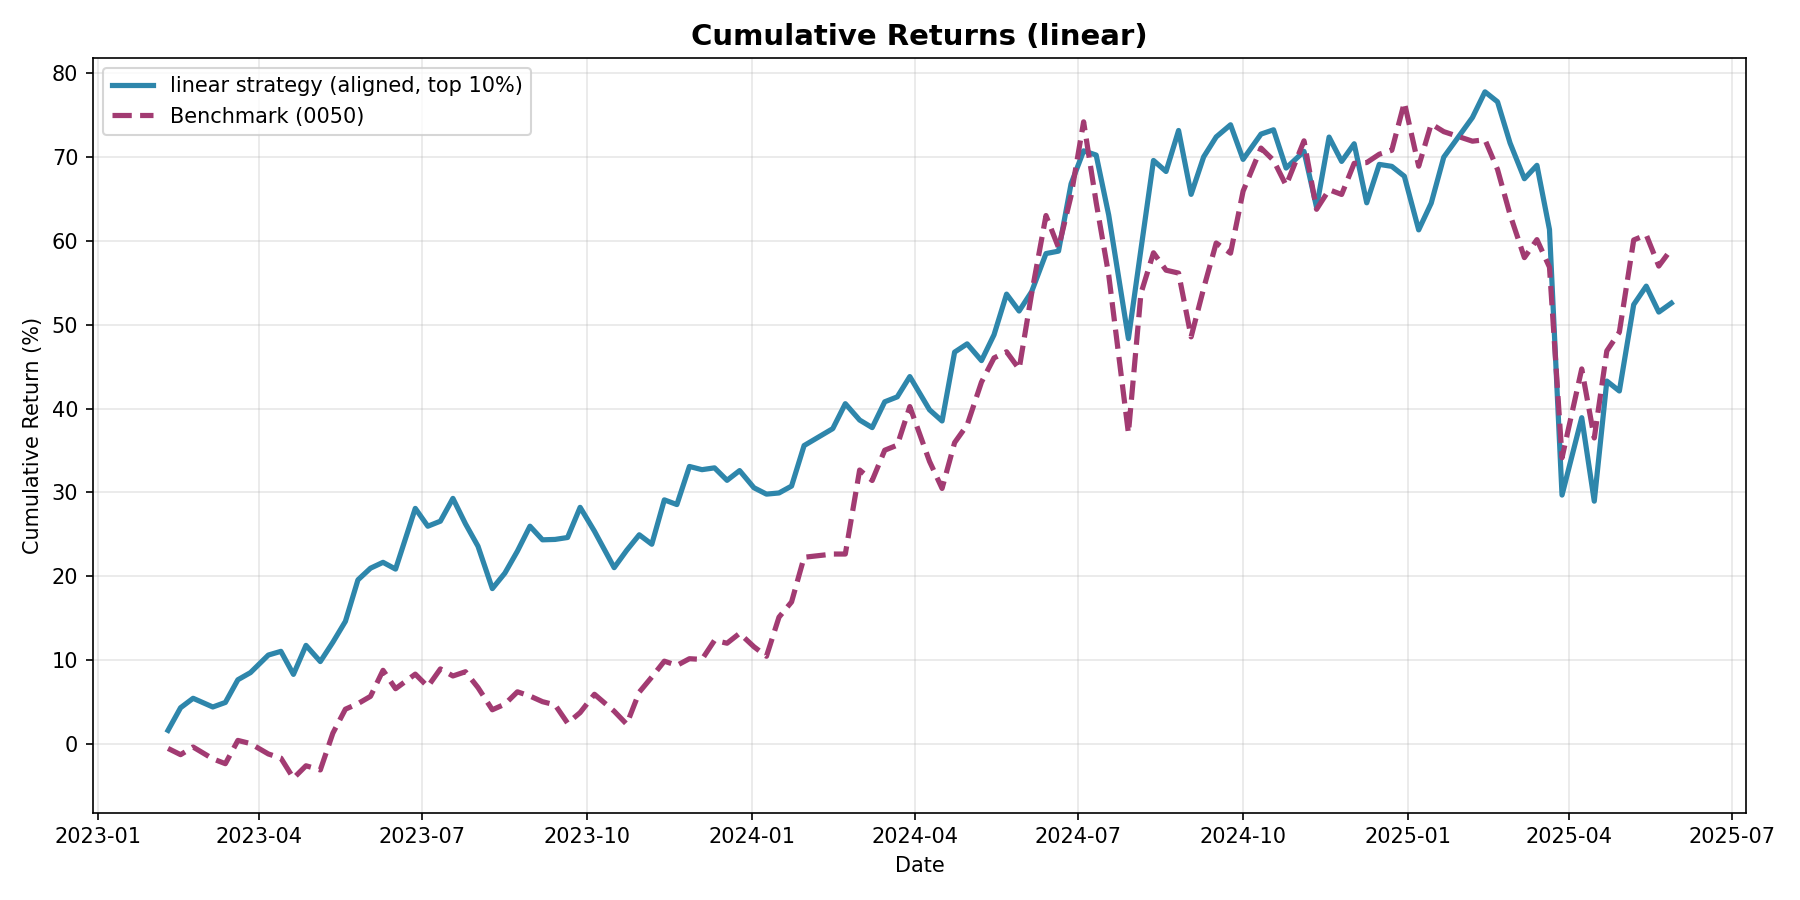
\includegraphics[width=\textwidth]{runs_gpu_static_to_20250601/static/long/baseline_linear/plots/cum_returns.png}
    \caption{Linear}
  \end{subfigure}
  \hfill
  \begin{subfigure}[t]{0.47\textwidth}
    \centering
    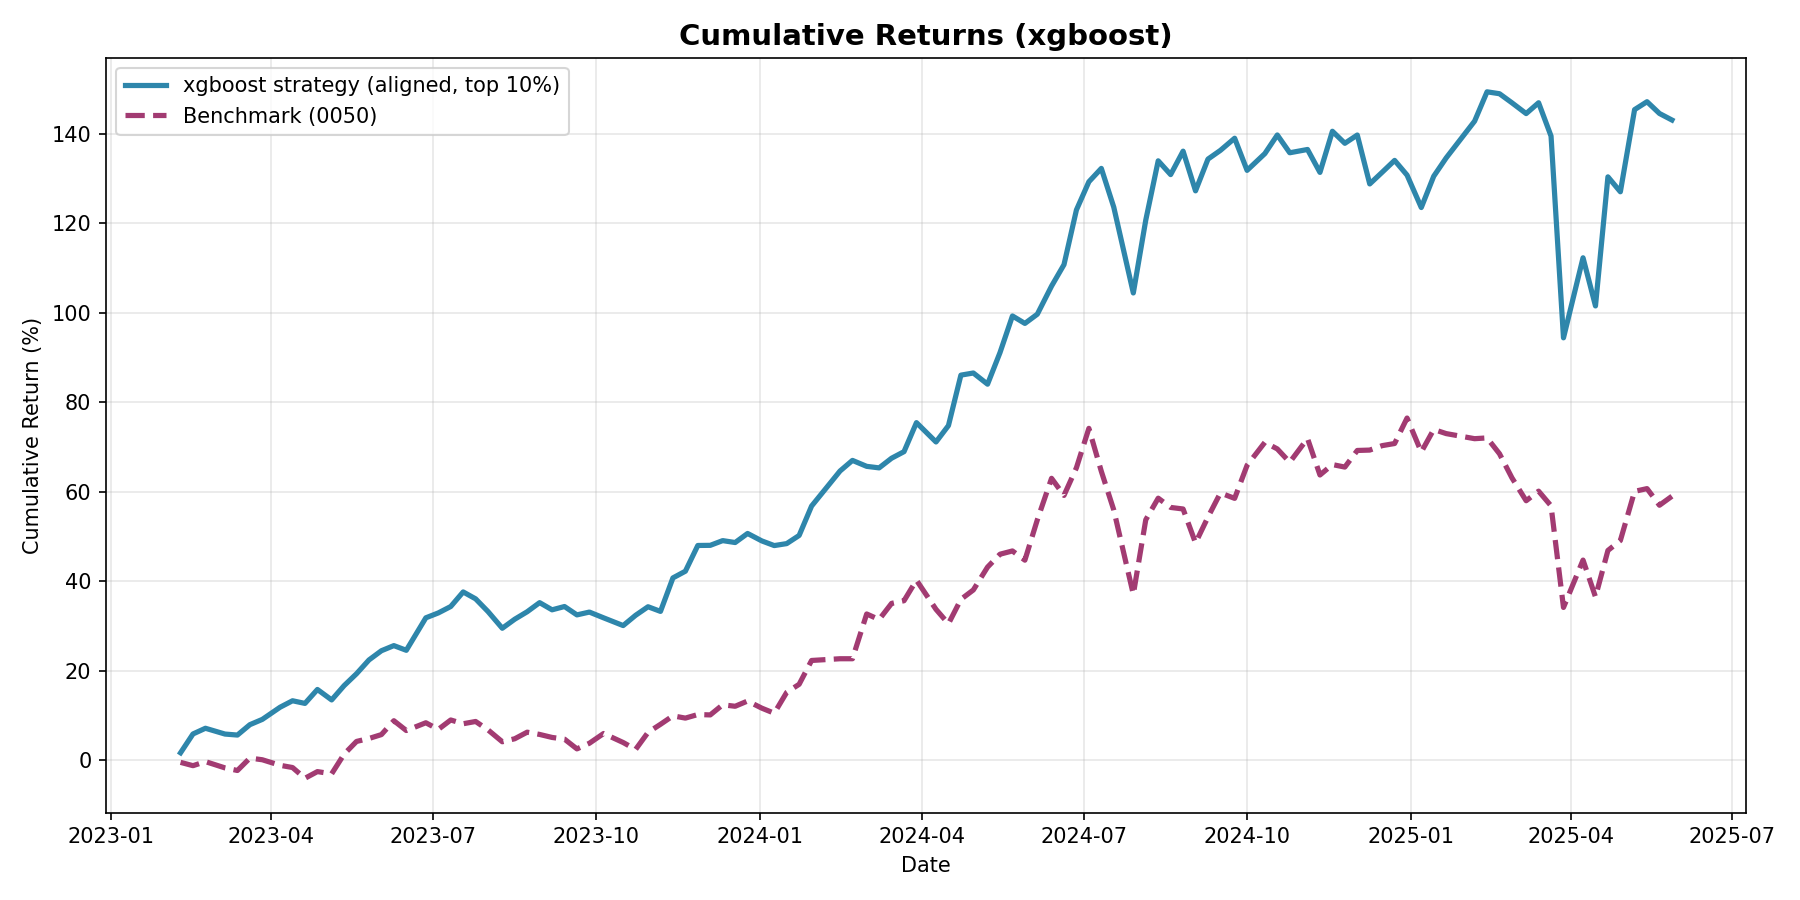
\includegraphics[width=\textwidth]{runs_gpu_static_to_20250601/static/long/baseline_xgboost/plots/cum_returns.png}
    \caption{XGBoost}
  \end{subfigure}
  \par\vspace{0.5em}
  \begin{subfigure}[t]{0.47\textwidth}
    \centering
    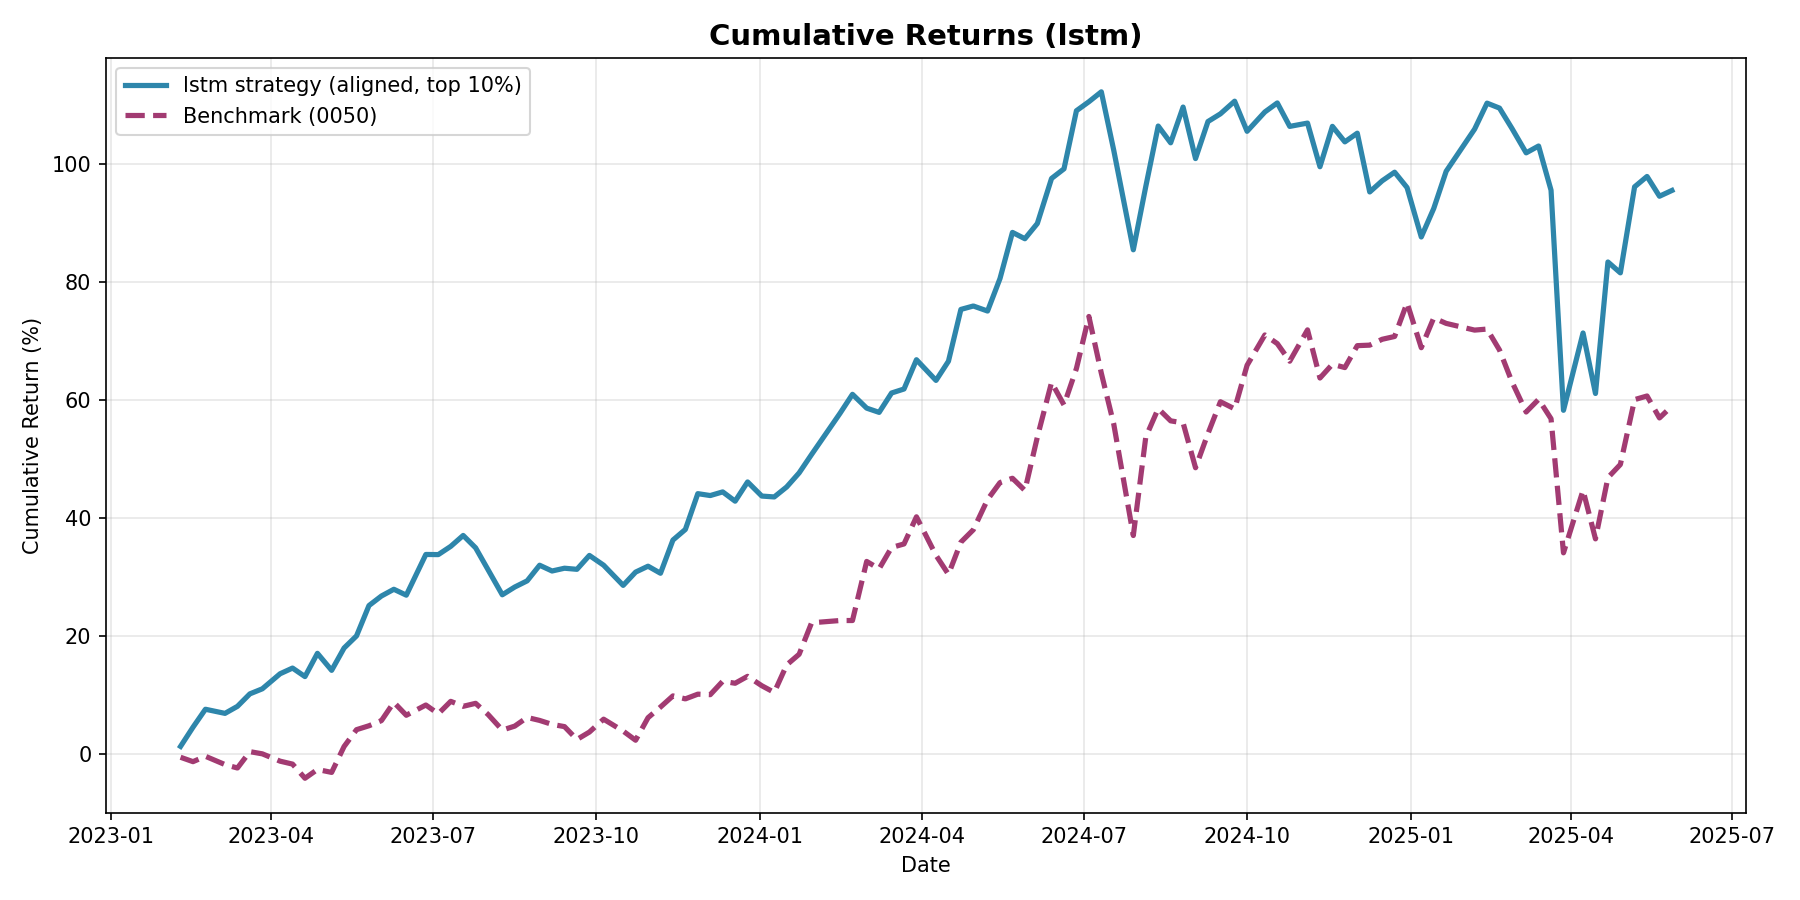
\includegraphics[width=\textwidth]{runs_gpu_static_to_20250601/static/long/baseline_lstm/plots/cum_returns.png}
    \caption{LSTM}
  \end{subfigure}
  \hfill
  \begin{subfigure}[t]{0.47\textwidth}
    \centering
    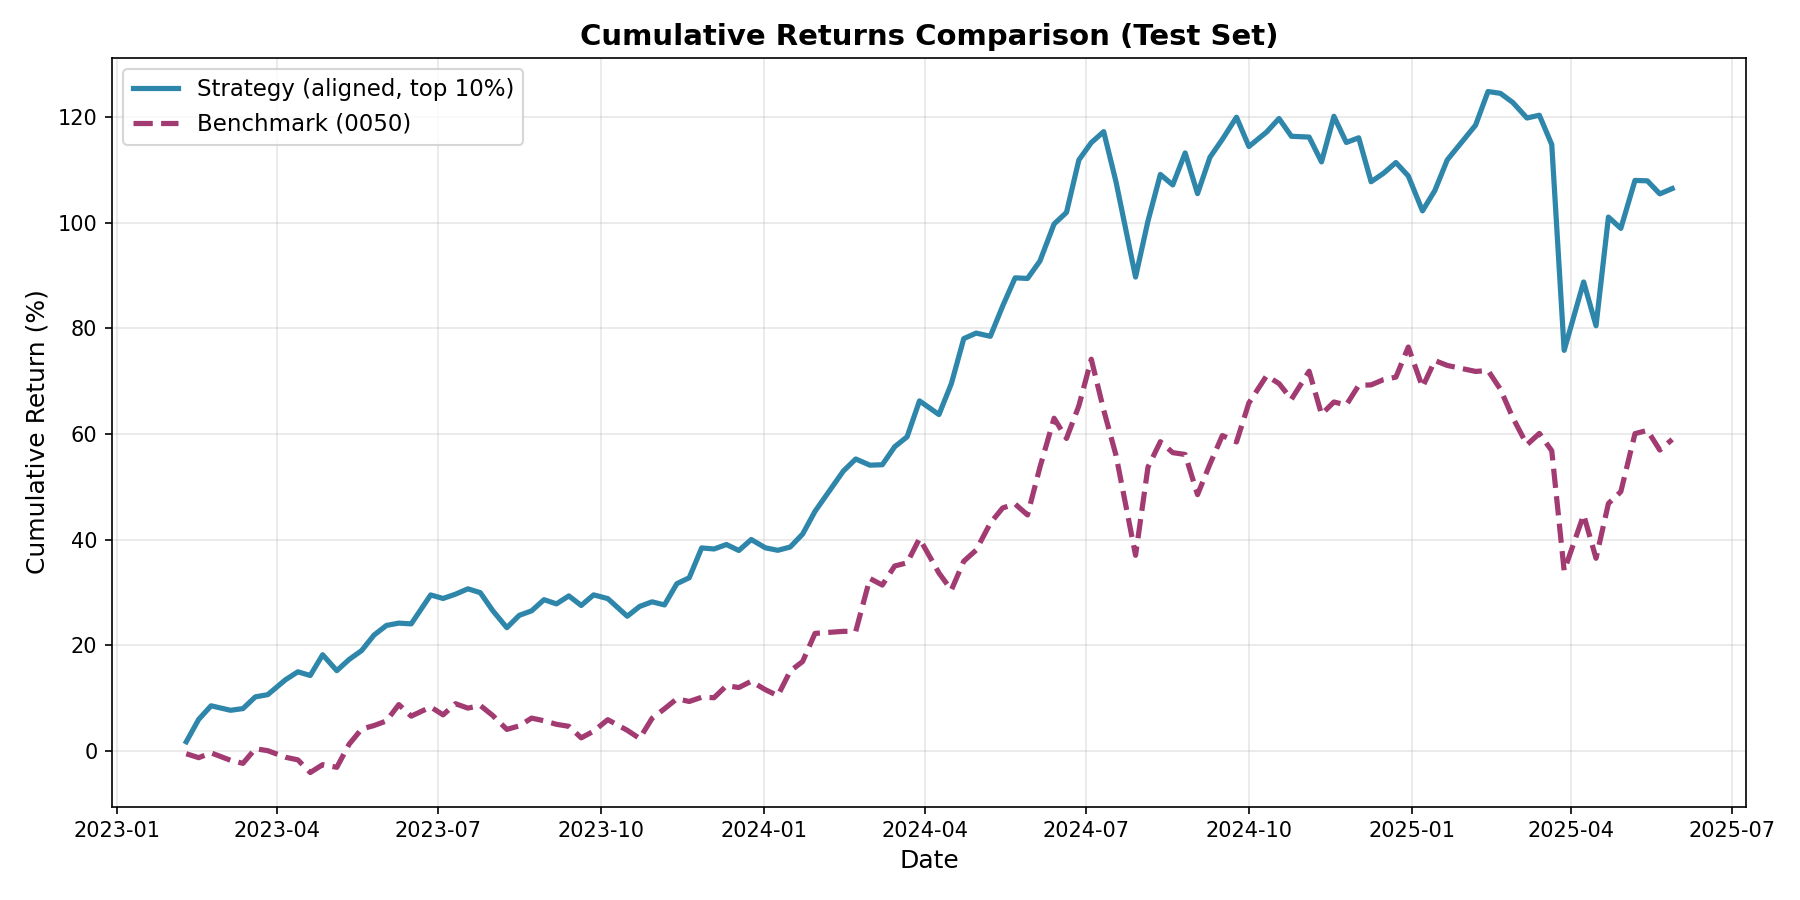
\includegraphics[width=\textwidth]{runs_gpu_static_to_20250601/static/long/mlp/plots/cum_returns.png}
    \caption{DNN}
  \end{subfigure}
  \par\vspace{0.5em}
  \begin{subfigure}[t]{0.47\textwidth}
    \centering
    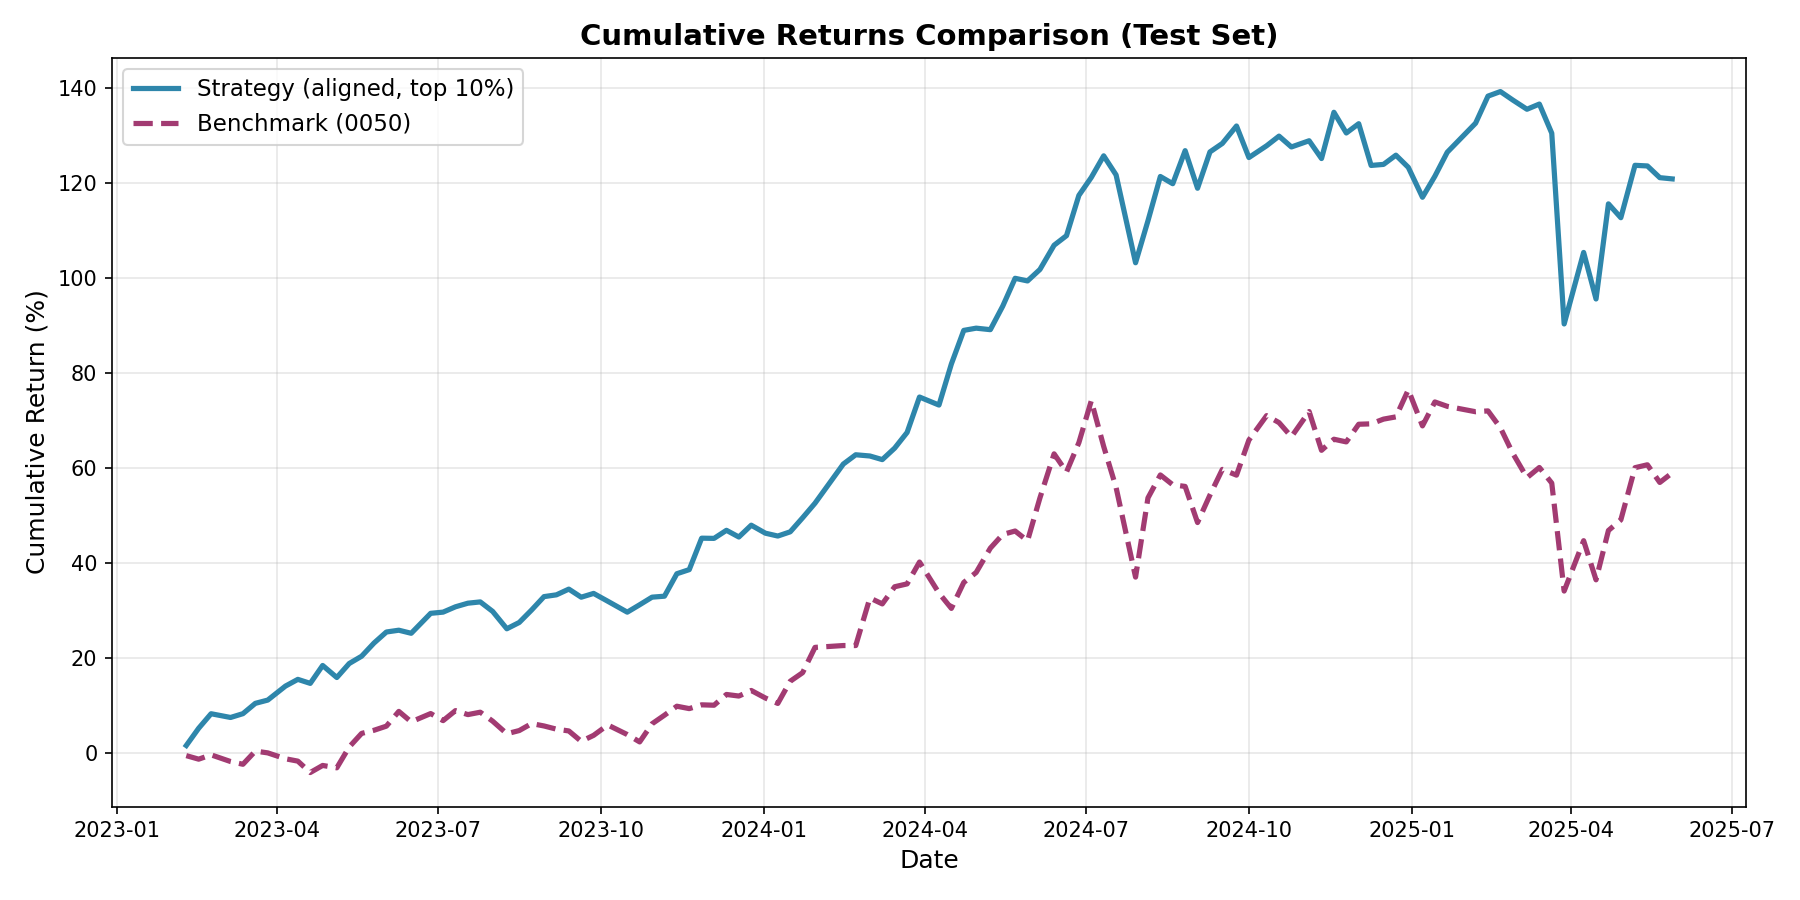
\includegraphics[width=\textwidth]{runs_gpu_static_to_20250601/static/long/gat_industry/plots/cum_returns.png}
    \caption{GAT-industry}
  \end{subfigure}
  \hfill
  \begin{subfigure}[t]{0.47\textwidth}
    \centering
    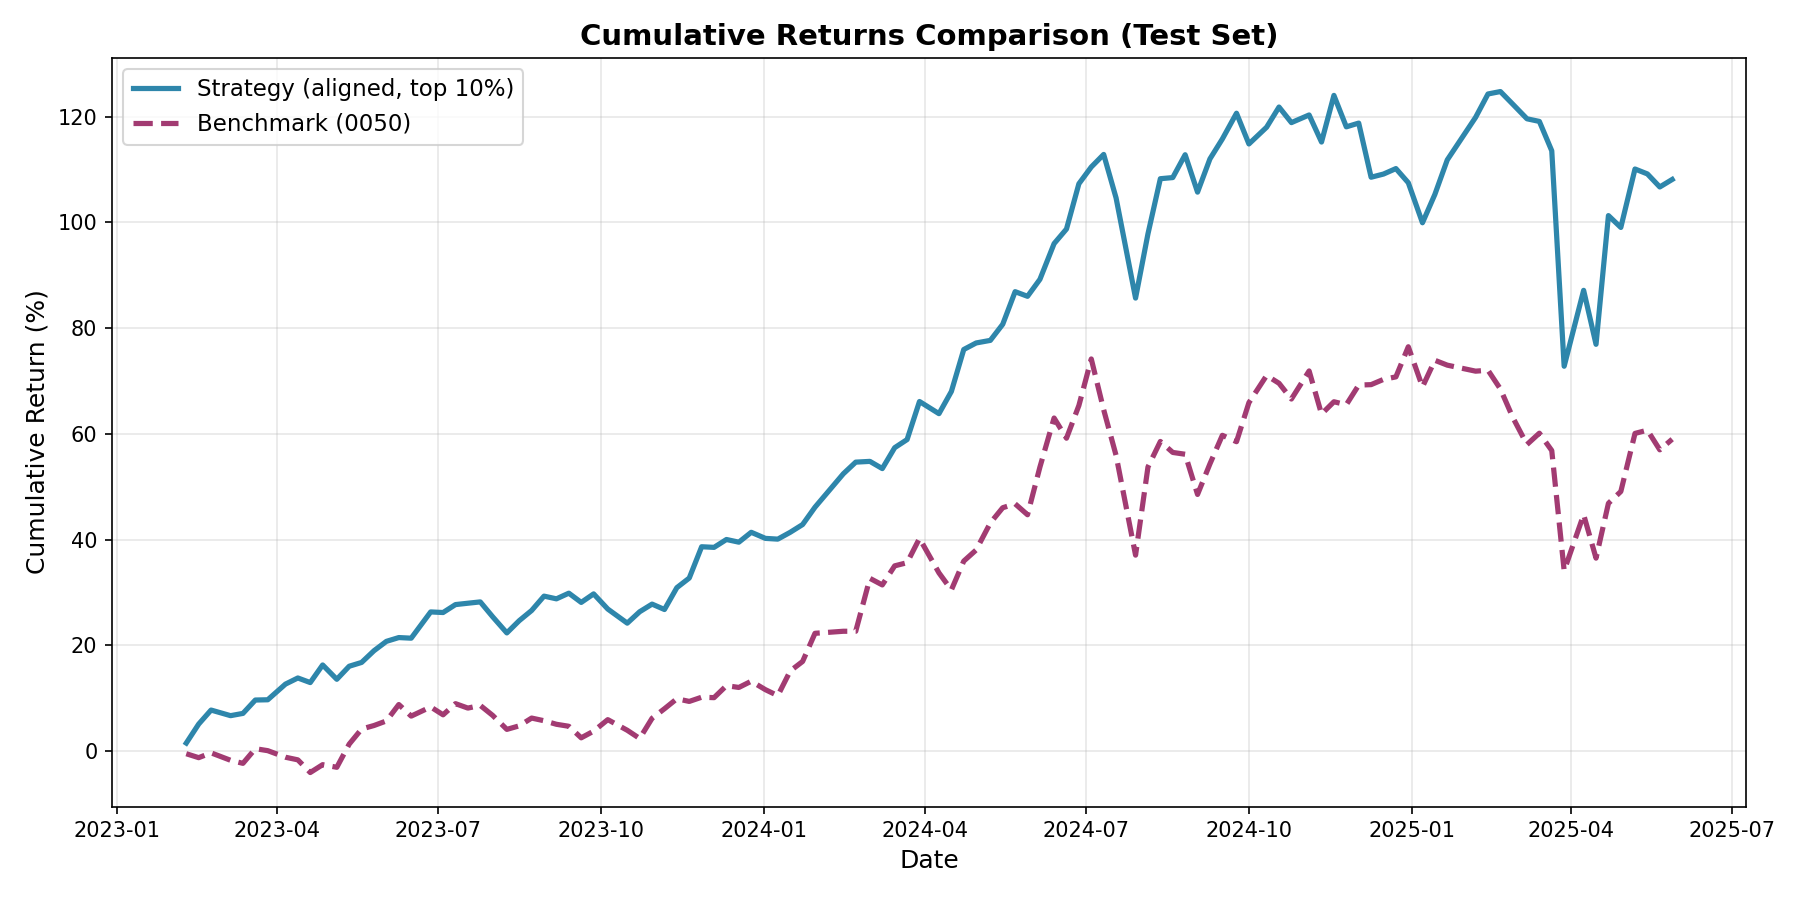
\includegraphics[width=\textwidth]{runs_gpu_static_to_20250601/static/long/gat_universe/plots/cum_returns.png}
    \caption{GAT-universe}
  \end{subfigure}
  \par\vspace{0.5em}
  \begin{subfigure}[t]{0.47\textwidth}
    \centering
    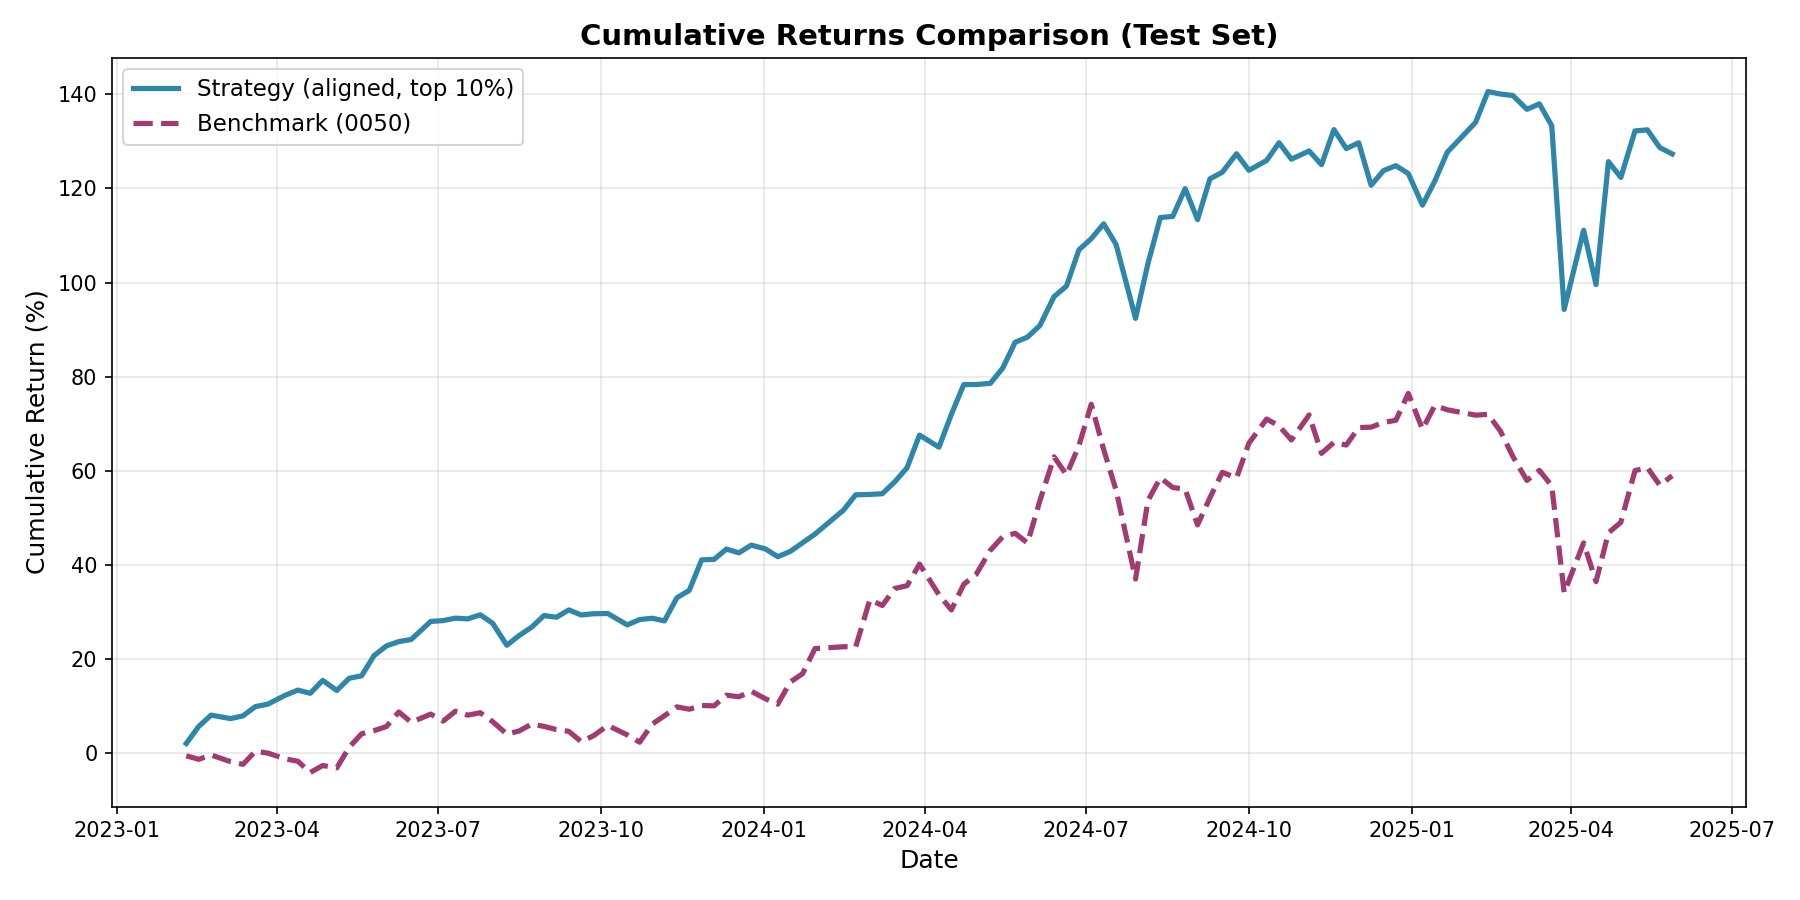
\includegraphics[width=\textwidth]{runs_gpu_static_to_20250601/static/long/gat_two_graph_no_neutral/plots/cum_returns.png}
    \caption{GAT-TwoGraph}
  \end{subfigure}
  \hfill
  \begin{subfigure}[t]{0.47\textwidth}
    \centering
    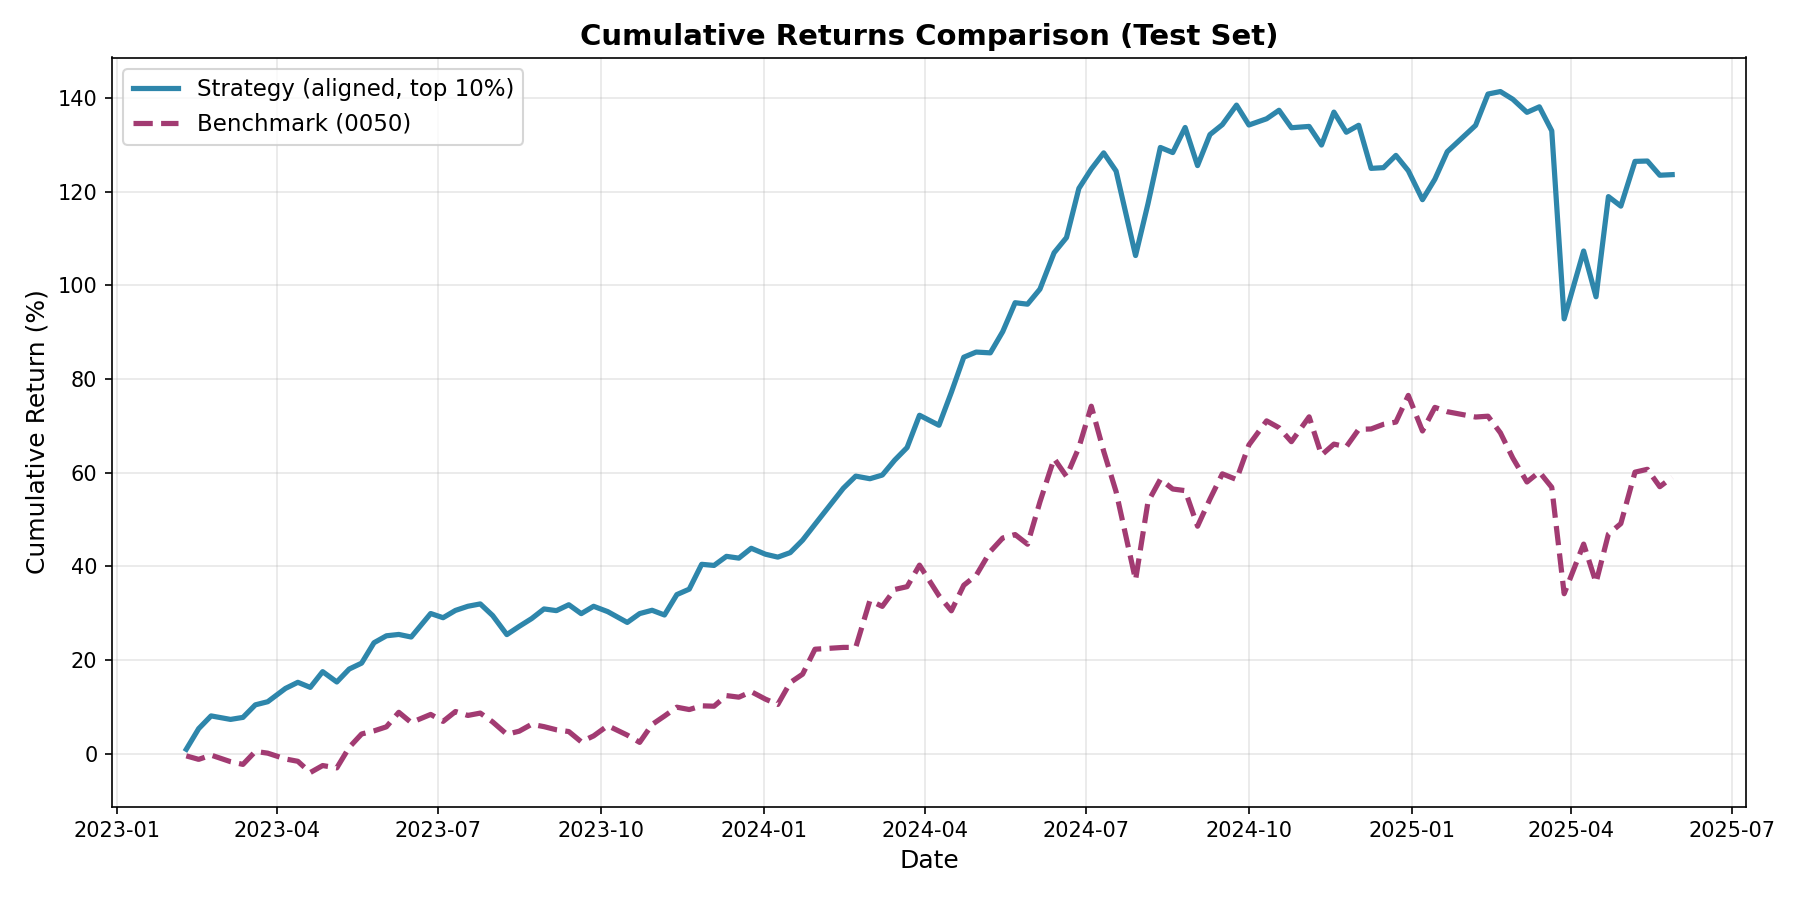
\includegraphics[width=\textwidth]{runs_gpu_static_to_20250601/static/long/dmfm_ind_neutral/plots/cum_returns.png}
    \caption{GAT-IndNeutral}
  \end{subfigure}
  \par\vspace{0.5em}
  \hfill
  \begin{subfigure}[t]{0.47\textwidth}
    \centering
    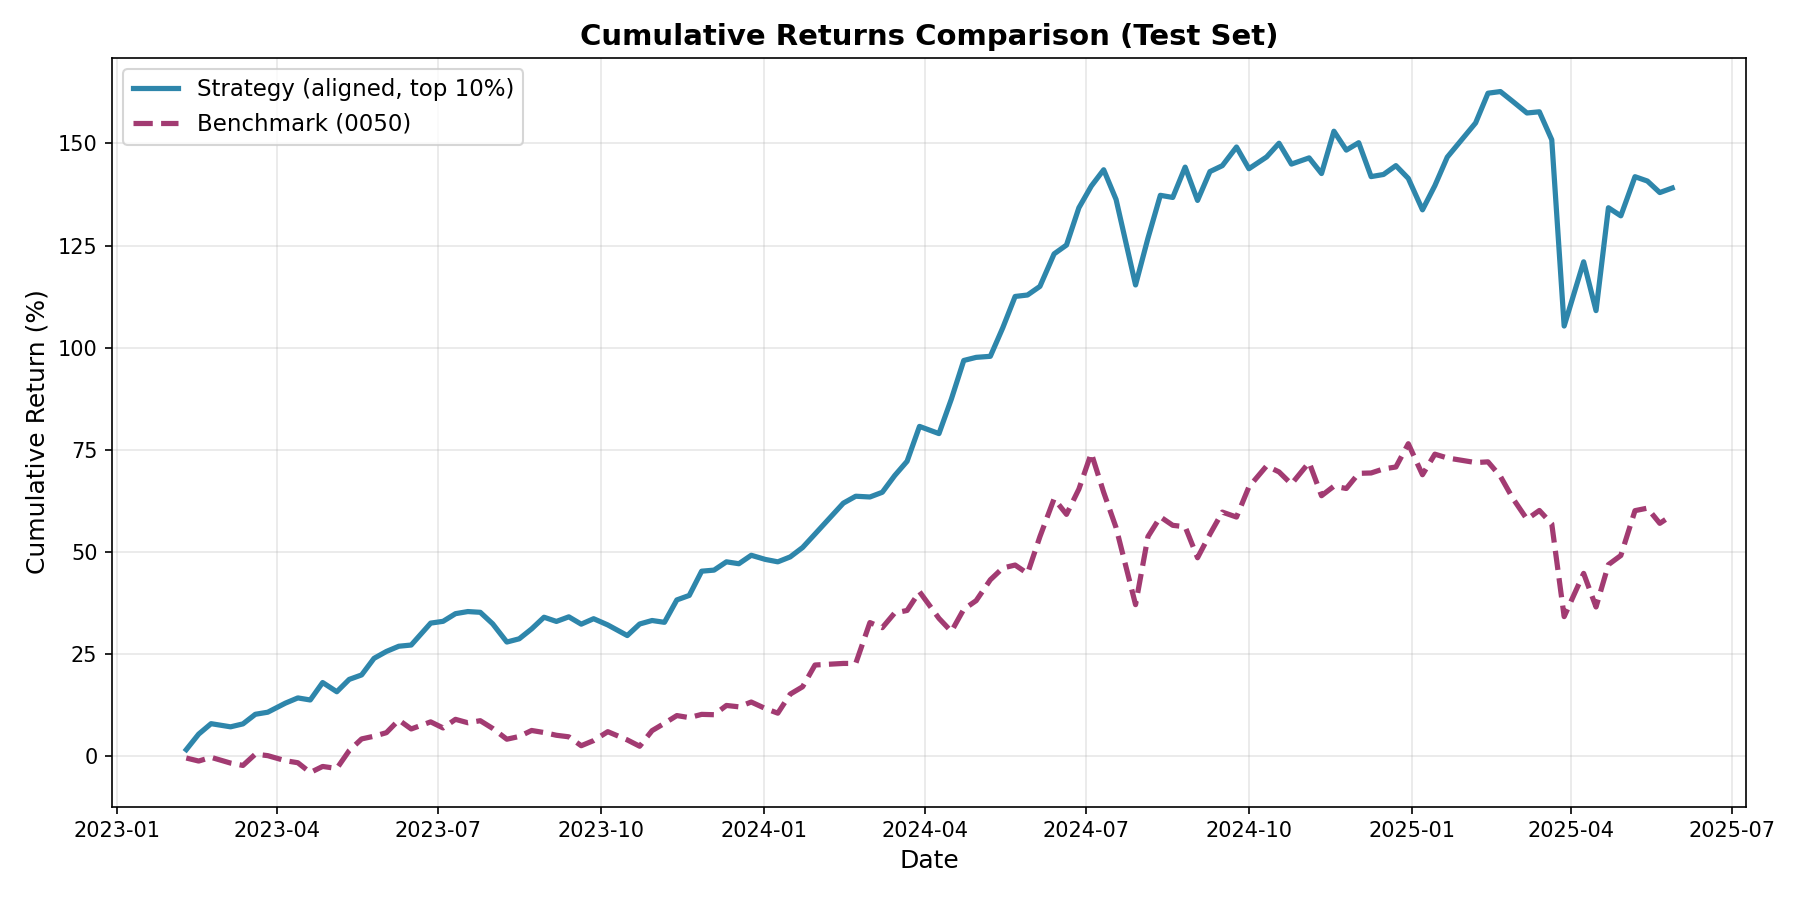
\includegraphics[width=\textwidth]{runs_gpu_static_to_20250601/static/long/dmfm_full/plots/cum_returns.png}
    \caption{GAT-full}
  \end{subfigure}
  \hfill
  \par\vspace{0.3em}
  \caption{Long window 各模型累積報酬曲線。}
  \label{fig:appendix_static_cum_returns_long}
\end{figure}

\clearpage
\subsection{Daily IC 補充結果}

\begin{figure}[H]
  \centering
  \captionsetup[subfigure]{font=small}
  \begin{subfigure}[t]{0.47\textwidth}
    \centering
    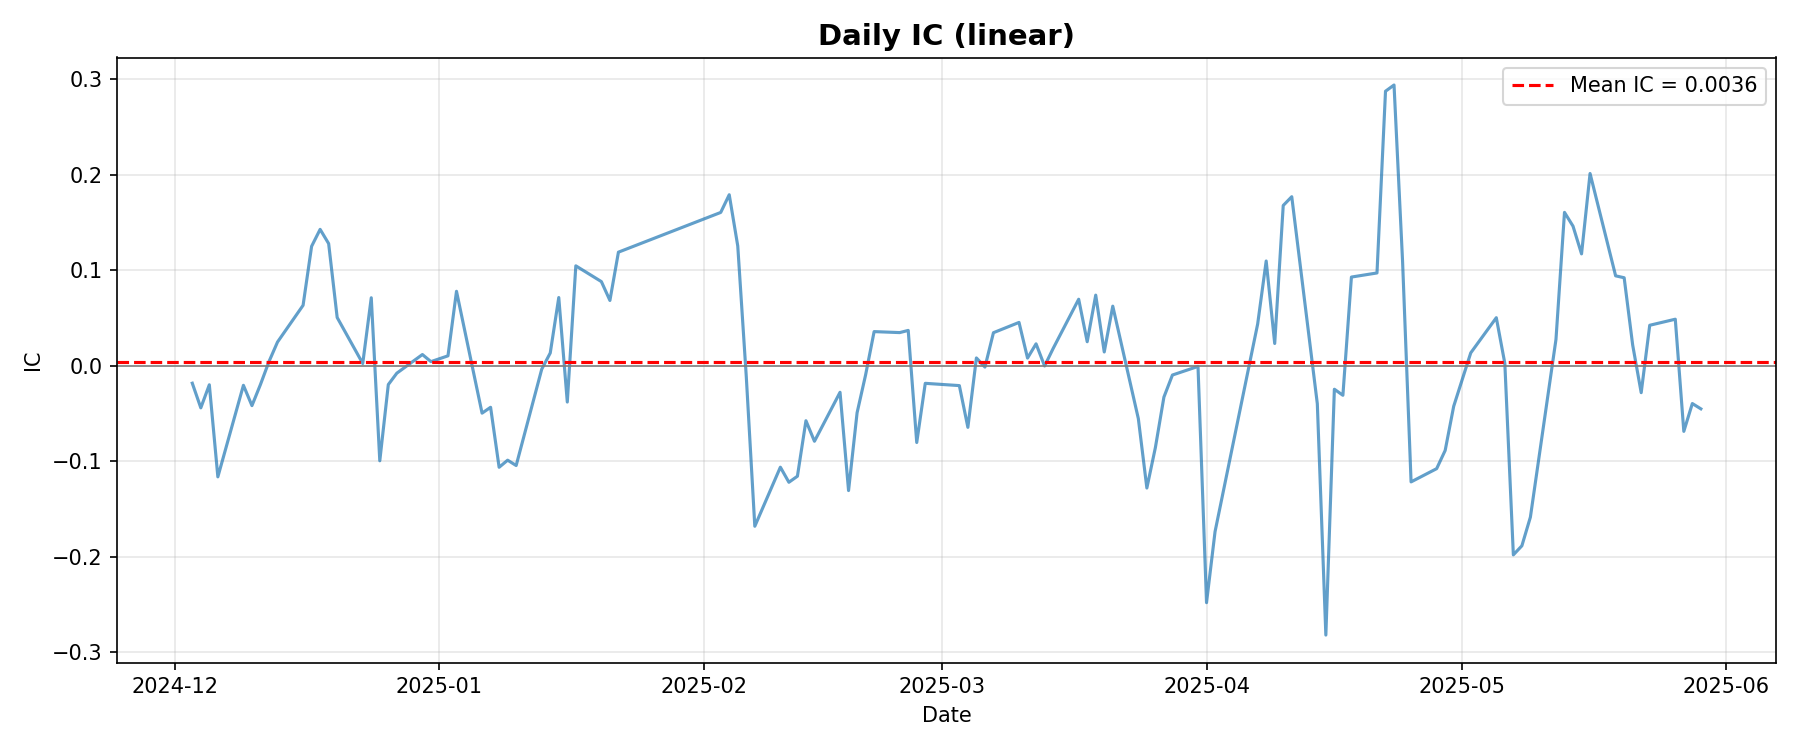
\includegraphics[width=\textwidth]{runs_gpu_static_to_20250601/static/short/baseline_linear/plots/daily_ic.png}
    \caption{Linear}
  \end{subfigure}
  \hfill
  \begin{subfigure}[t]{0.47\textwidth}
    \centering
    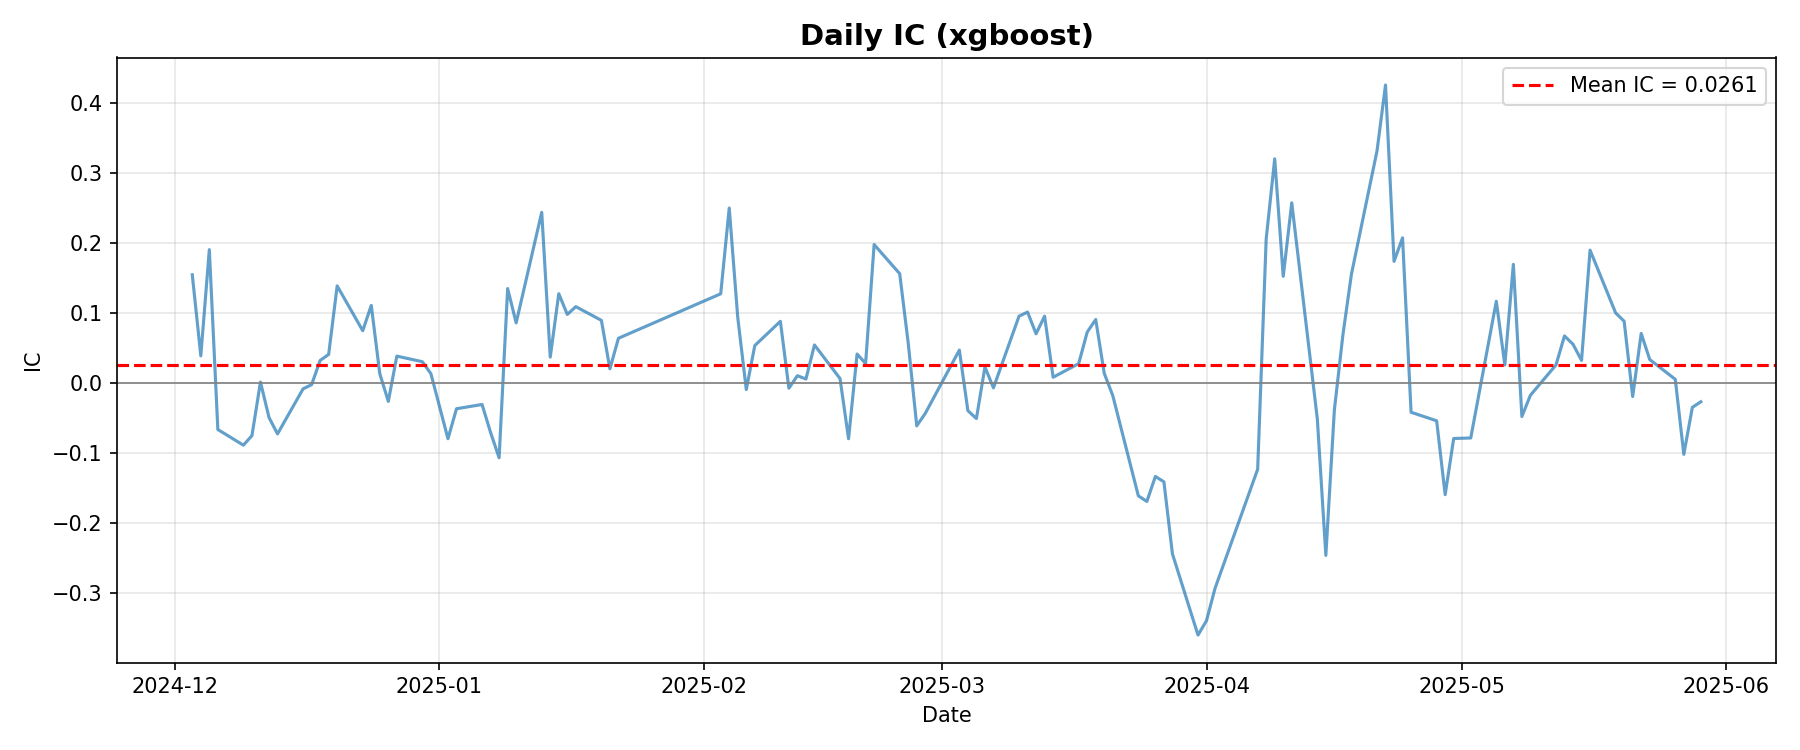
\includegraphics[width=\textwidth]{runs_gpu_static_to_20250601/static/short/baseline_xgboost/plots/daily_ic.png}
    \caption{XGBoost}
  \end{subfigure}
  \par\vspace{0.5em}
  \begin{subfigure}[t]{0.47\textwidth}
    \centering
    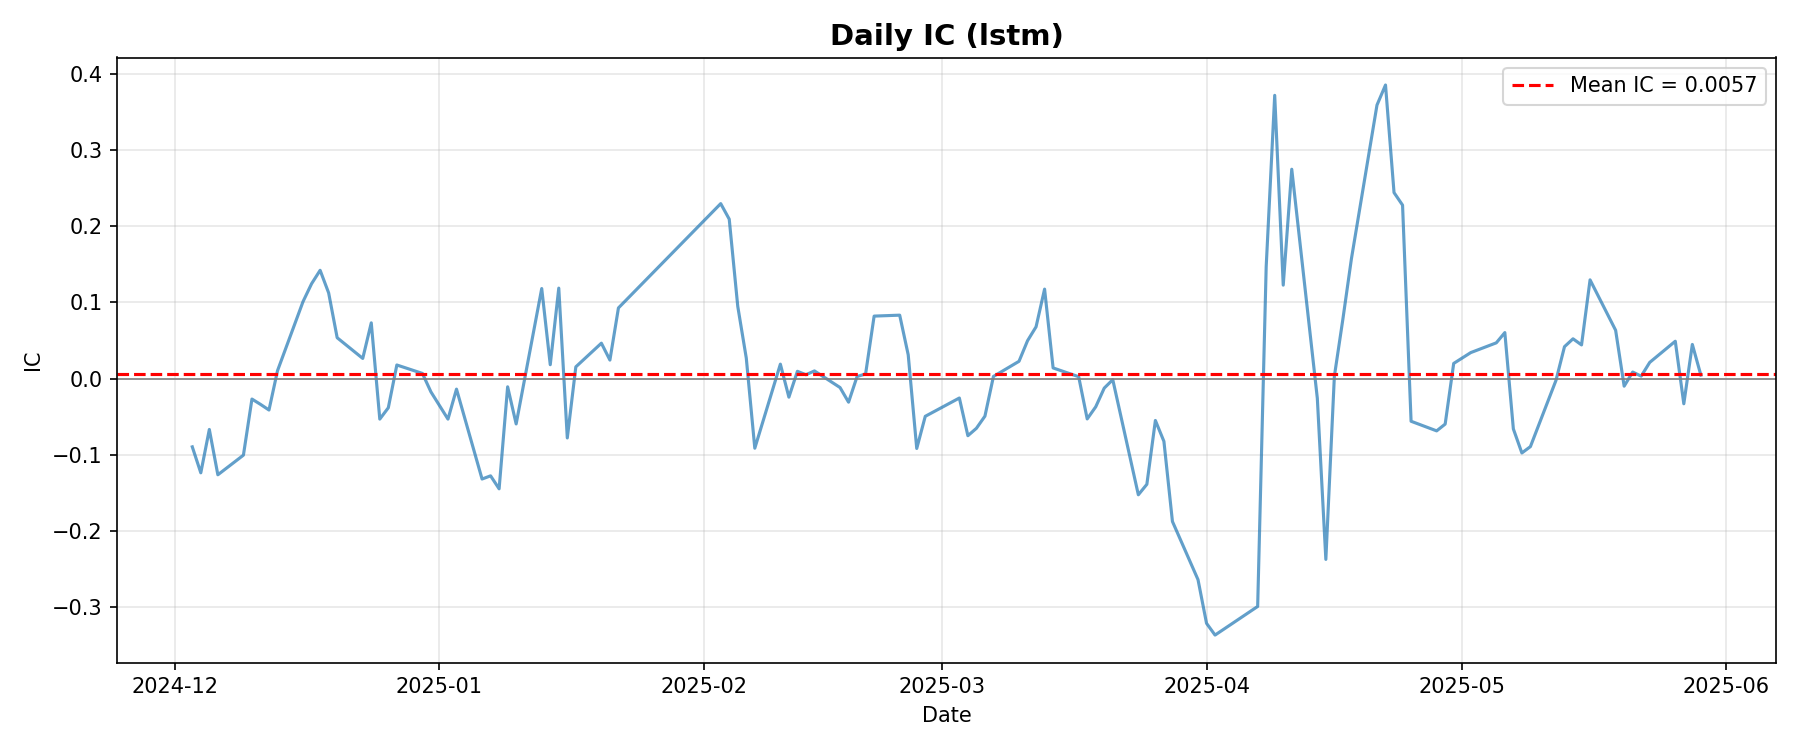
\includegraphics[width=\textwidth]{runs_gpu_static_to_20250601/static/short/baseline_lstm/plots/daily_ic.png}
    \caption{LSTM}
  \end{subfigure}
  \hfill
  \begin{subfigure}[t]{0.47\textwidth}
    \centering
    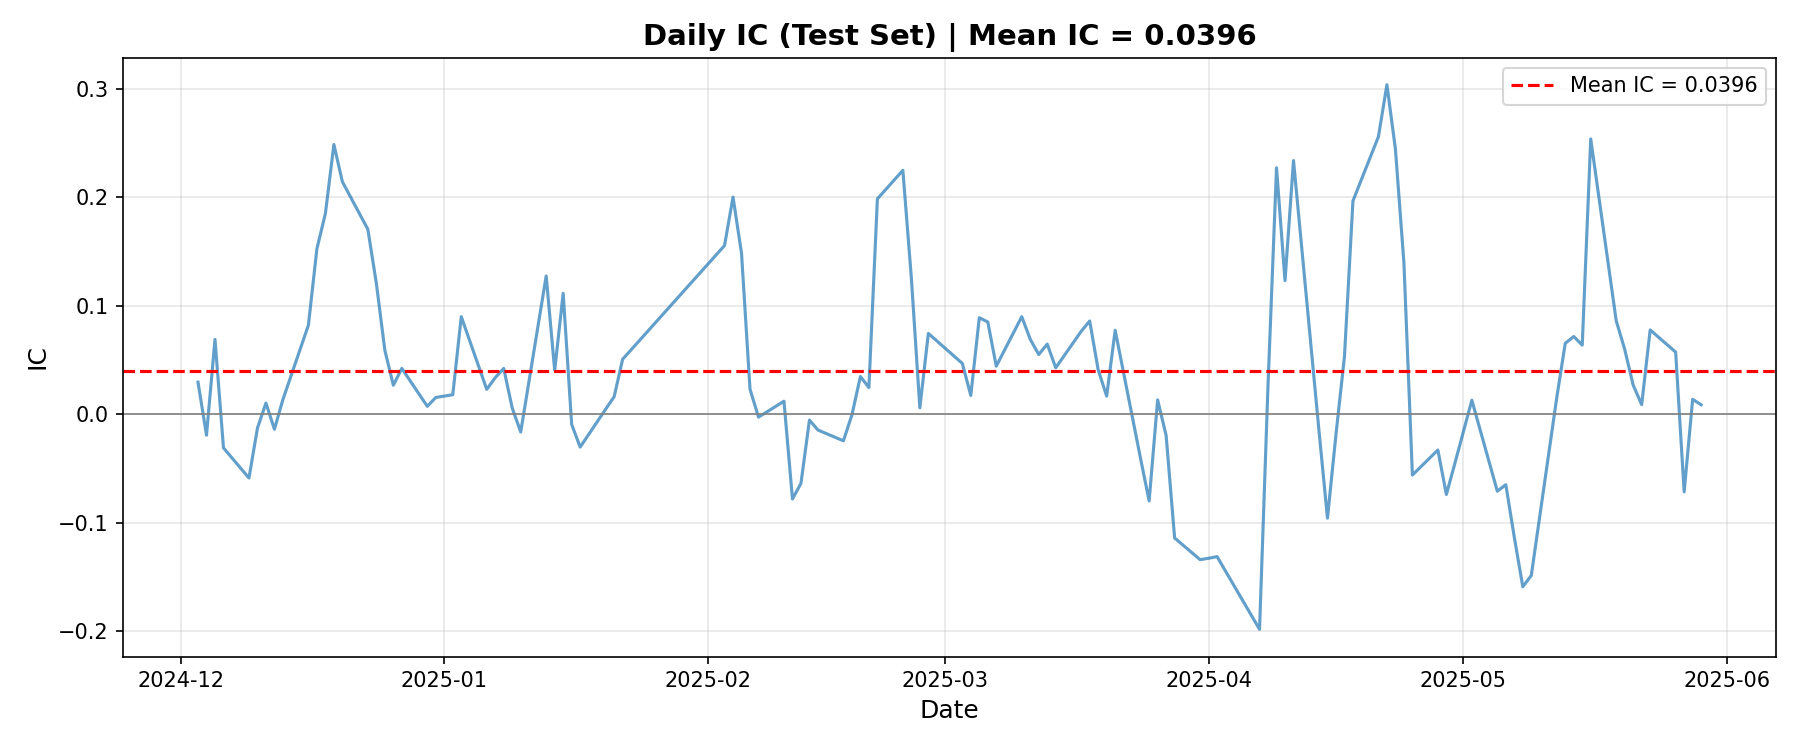
\includegraphics[width=\textwidth]{runs_gpu_static_to_20250601/static/short/mlp/plots/daily_ic.png}
    \caption{DNN}
  \end{subfigure}
  \par\vspace{0.5em}
  \begin{subfigure}[t]{0.47\textwidth}
    \centering
    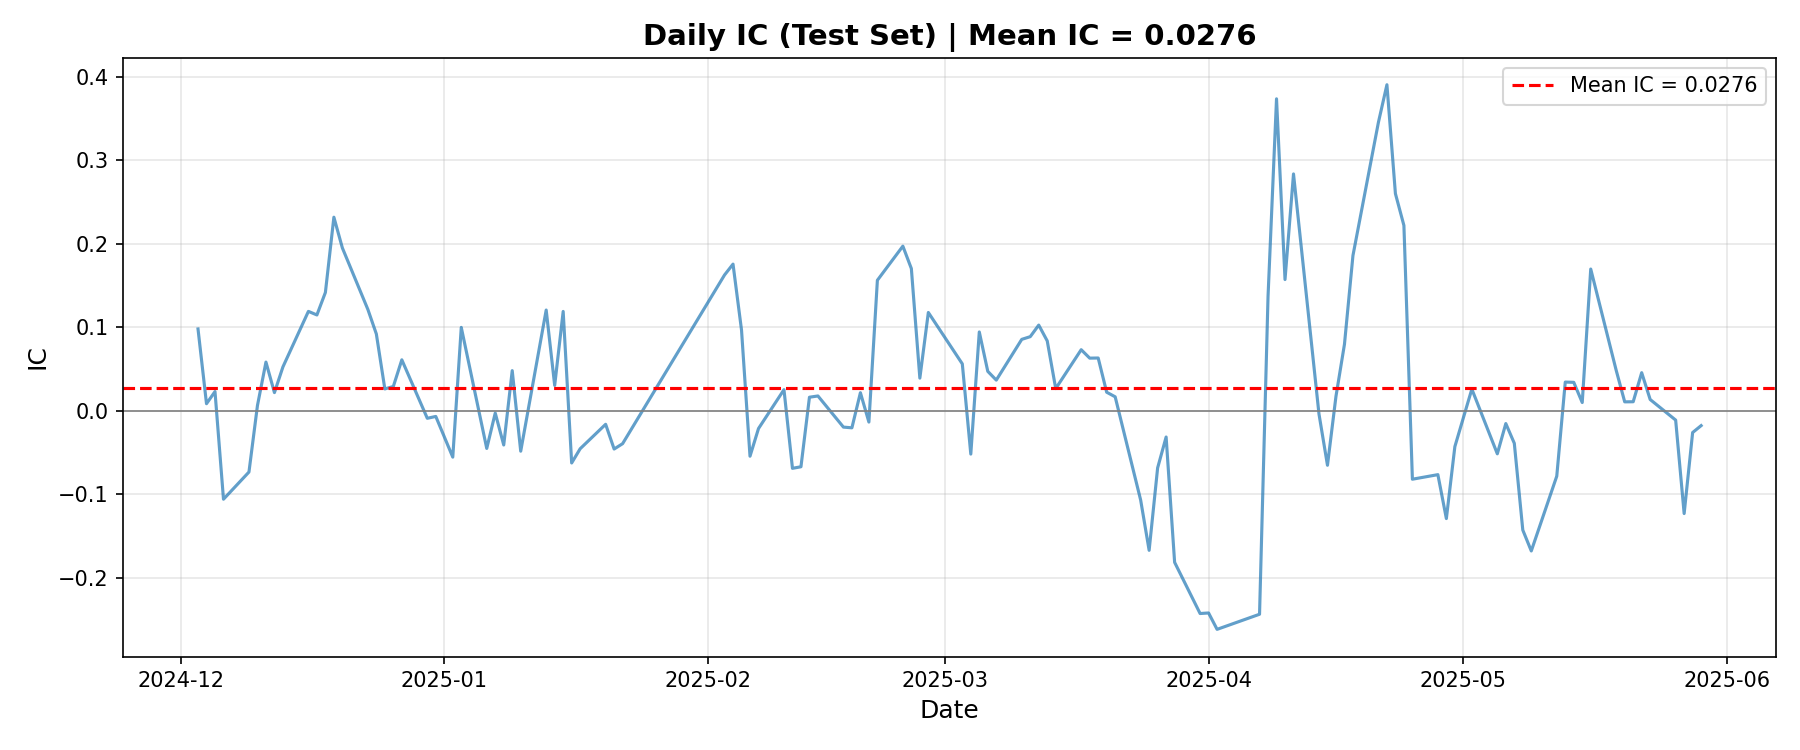
\includegraphics[width=\textwidth]{runs_gpu_static_to_20250601/static/short/gat_industry/plots/daily_ic.png}
    \caption{GAT-industry}
  \end{subfigure}
  \hfill
  \begin{subfigure}[t]{0.47\textwidth}
    \centering
    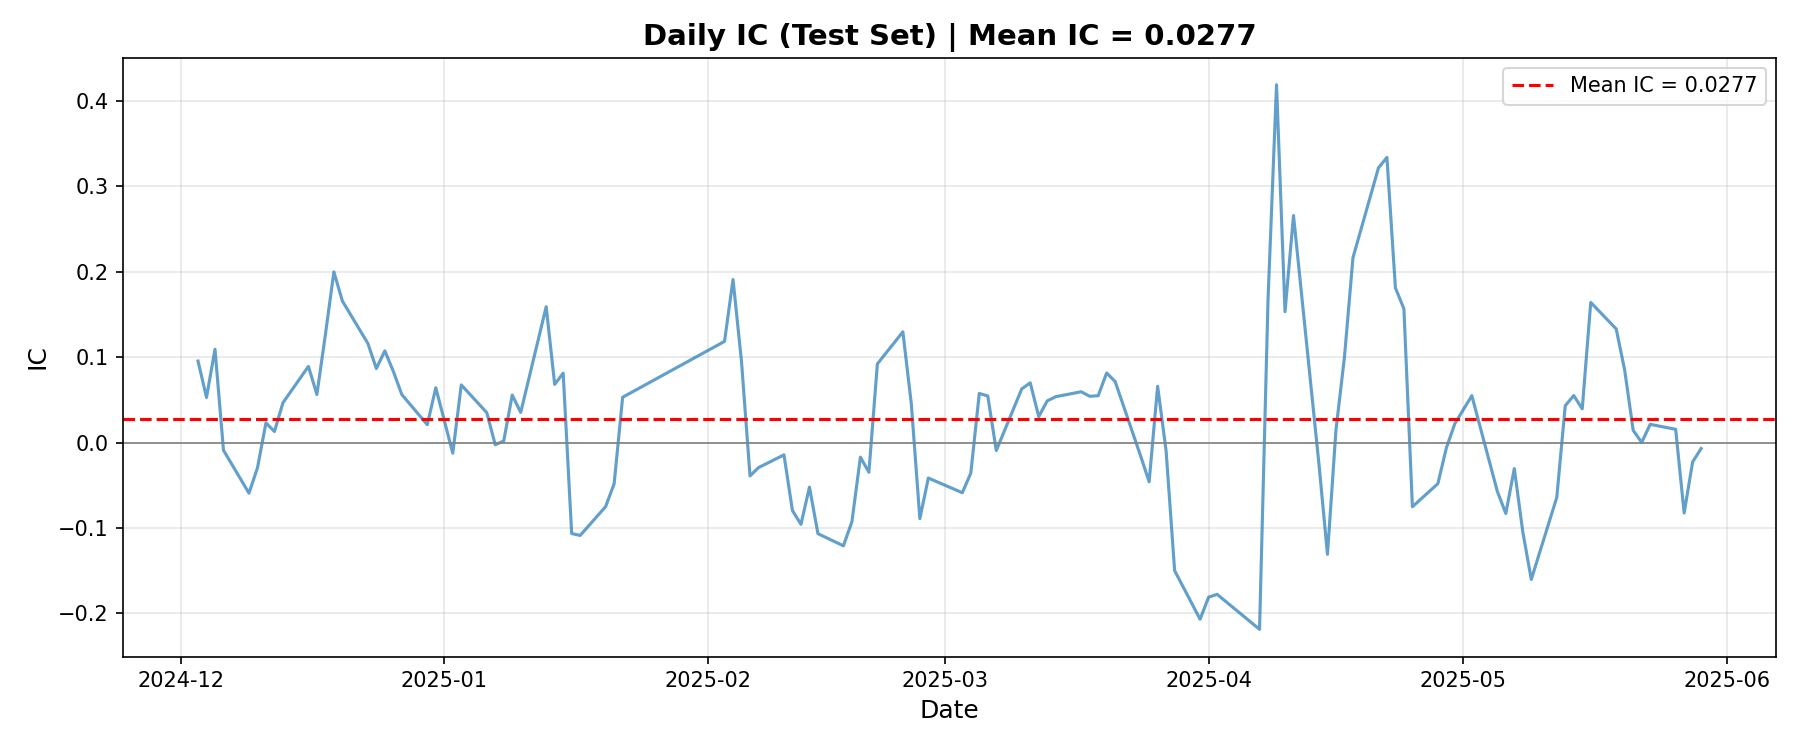
\includegraphics[width=\textwidth]{runs_gpu_static_to_20250601/static/short/gat_universe/plots/daily_ic.png}
    \caption{GAT-universe}
  \end{subfigure}
  \par\vspace{0.5em}
  \begin{subfigure}[t]{0.47\textwidth}
    \centering
    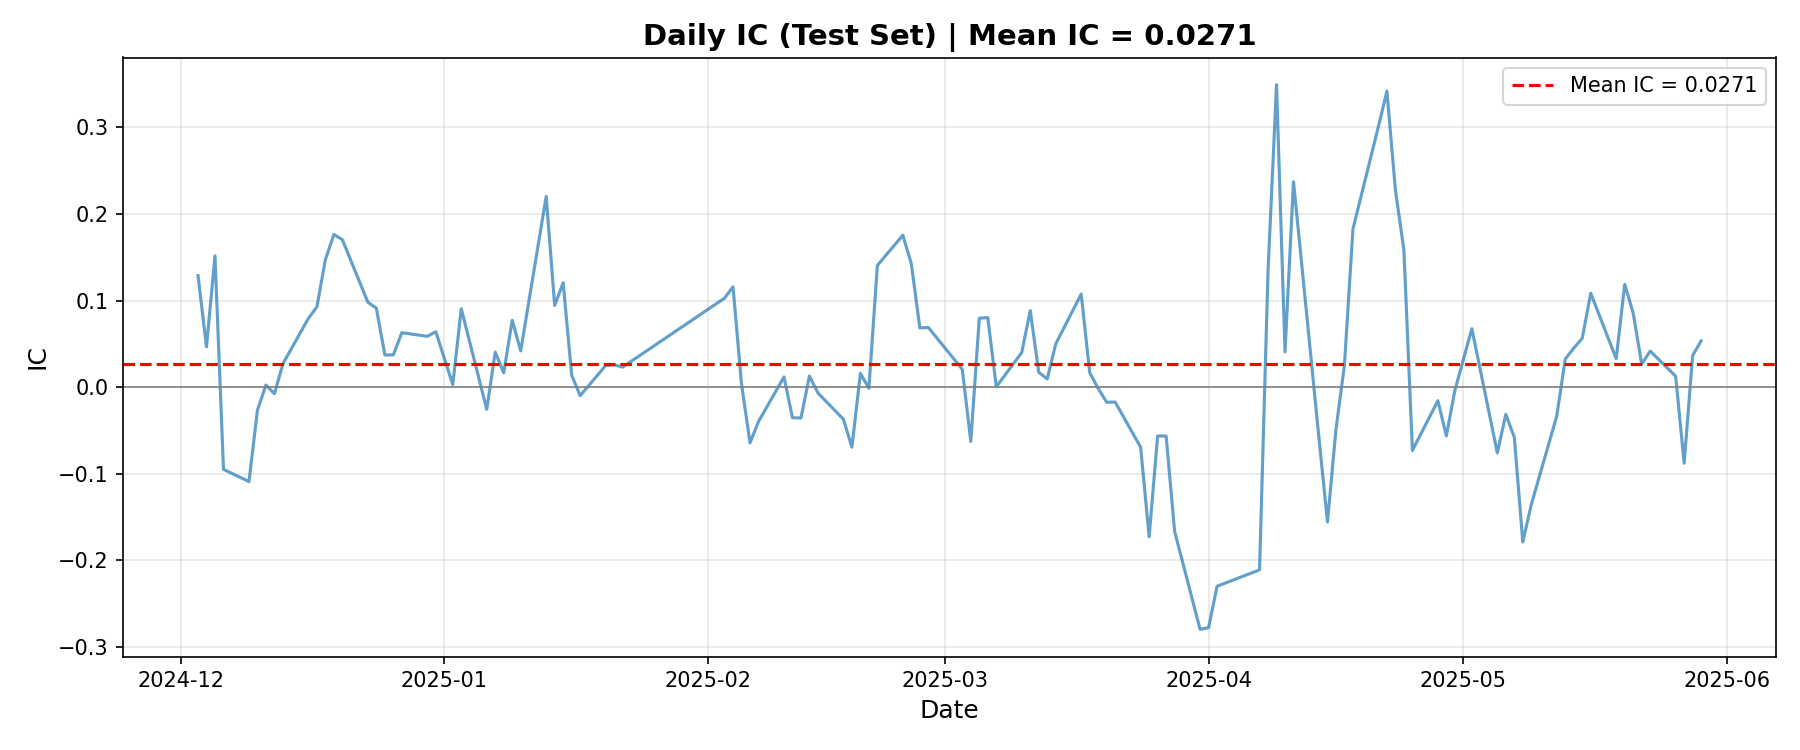
\includegraphics[width=\textwidth]{runs_gpu_static_to_20250601/static/short/gat_two_graph_no_neutral/plots/daily_ic.png}
    \caption{GAT-TwoGraph}
  \end{subfigure}
  \hfill
  \begin{subfigure}[t]{0.47\textwidth}
    \centering
    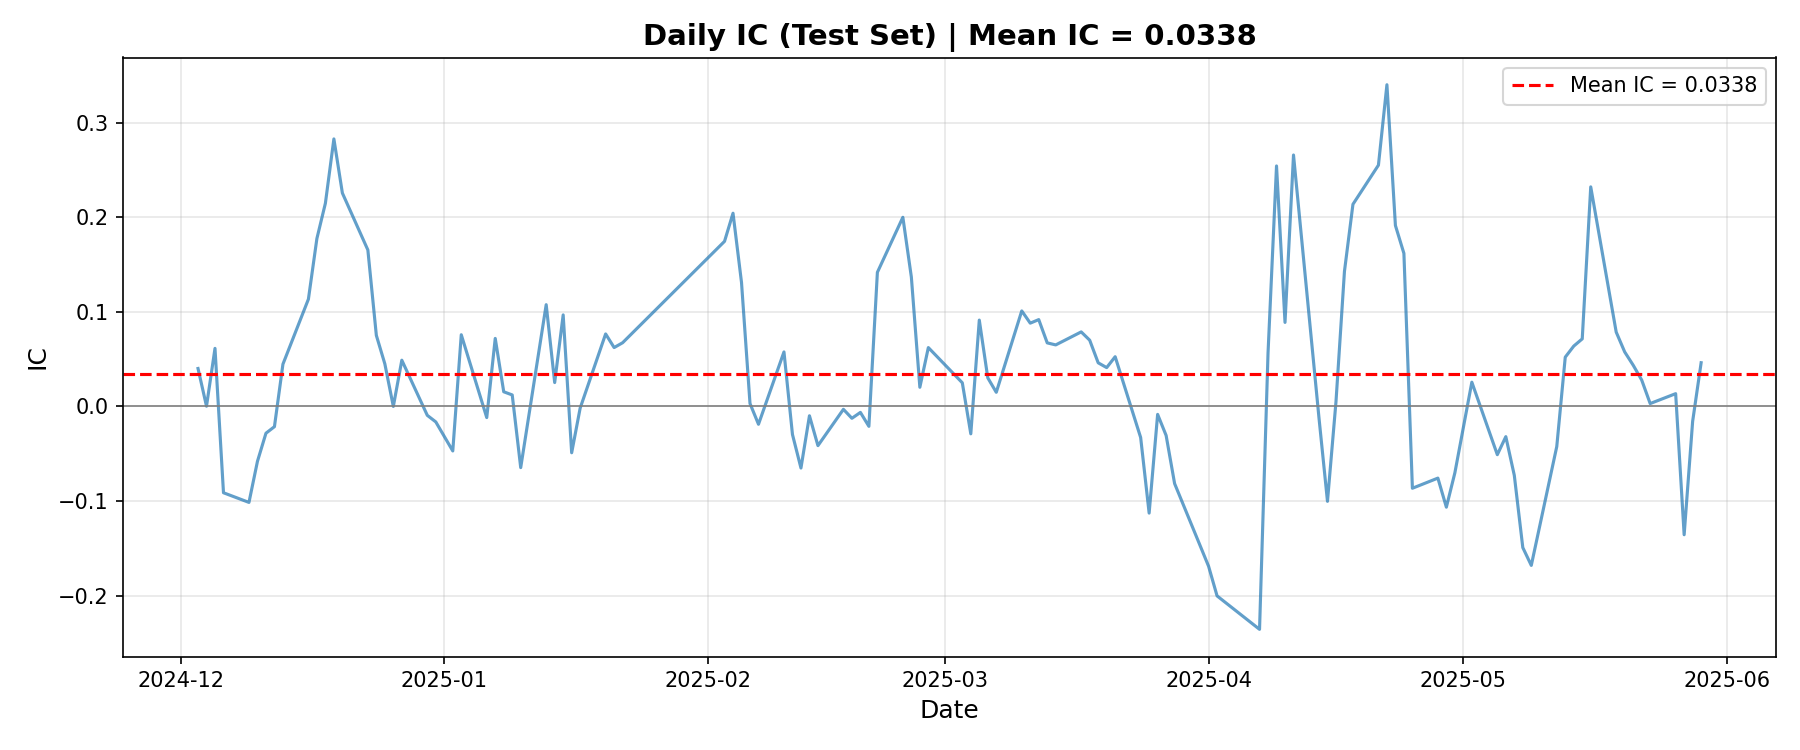
\includegraphics[width=\textwidth]{runs_gpu_static_to_20250601/static/short/dmfm_ind_neutral/plots/daily_ic.png}
    \caption{GAT-IndNeutral}
  \end{subfigure}
  \par\vspace{0.5em}
  \hfill
  \begin{subfigure}[t]{0.47\textwidth}
    \centering
    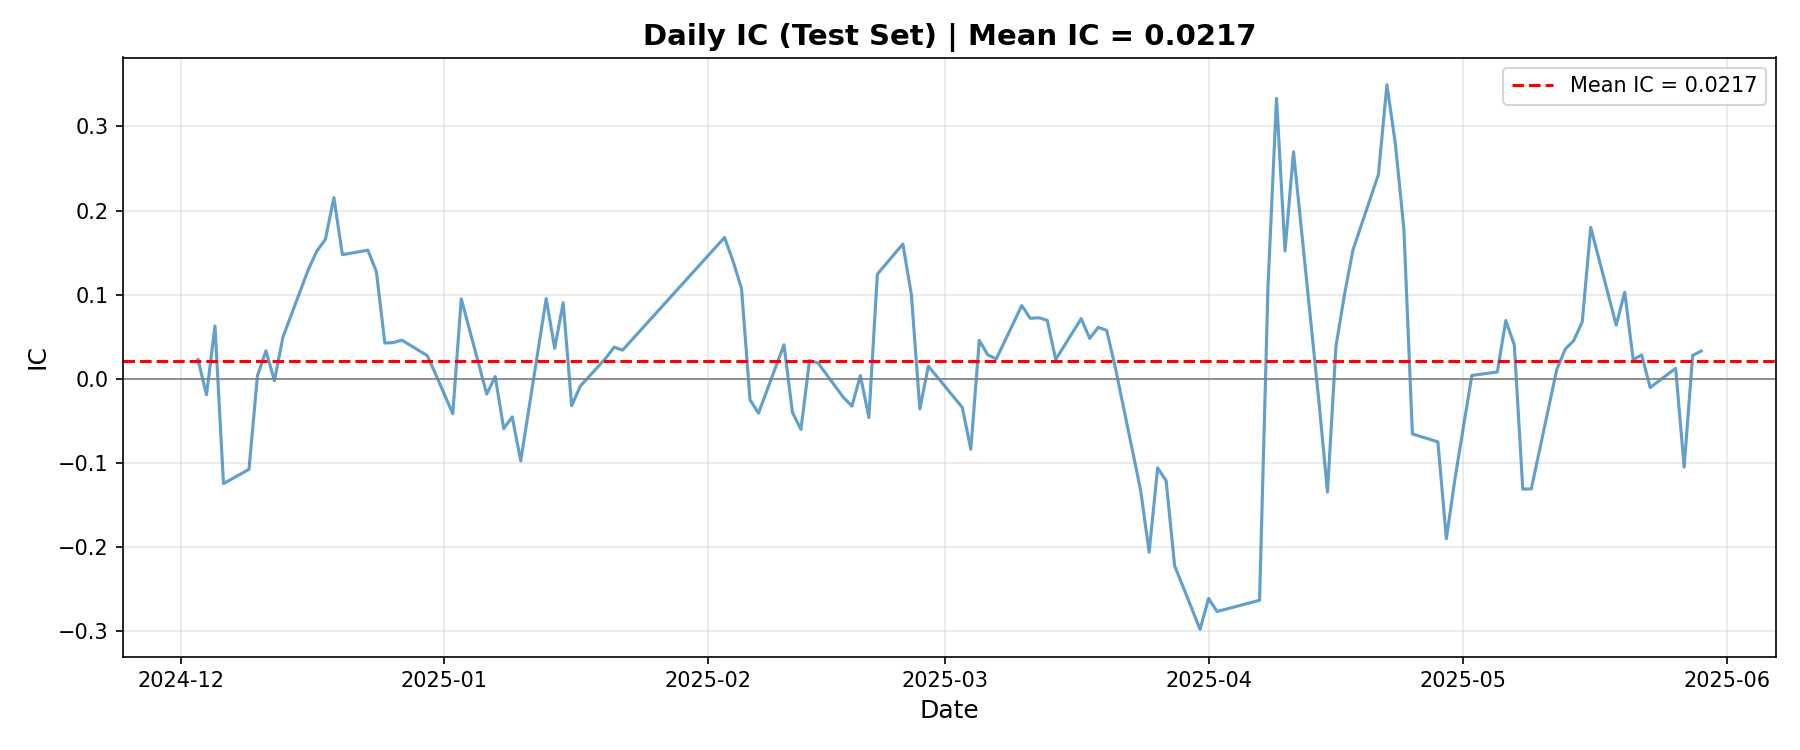
\includegraphics[width=\textwidth]{runs_gpu_static_to_20250601/static/short/dmfm_full/plots/daily_ic.png}
    \caption{GAT-full}
  \end{subfigure}
  \hfill
  \par\vspace{0.3em}
  \caption{Short window 各模型 Daily IC 時序。}
  \label{fig:appendix_static_daily_ic_short}
\end{figure}

\clearpage
\begin{figure}[H]
  \centering
  \captionsetup[subfigure]{font=small}
  \begin{subfigure}[t]{0.47\textwidth}
    \centering
    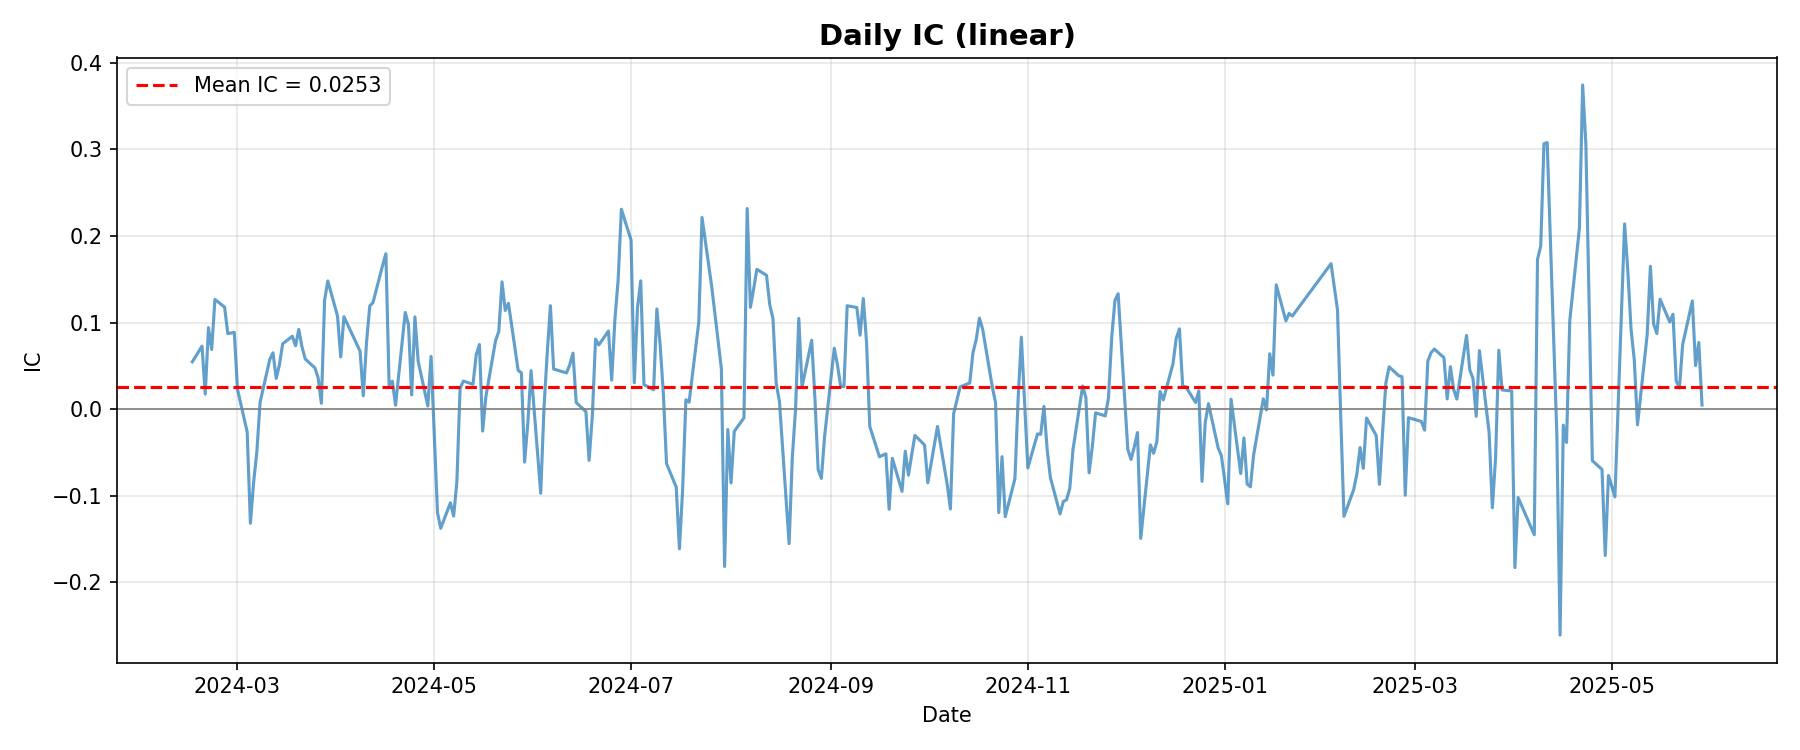
\includegraphics[width=\textwidth]{runs_gpu_static_to_20250601/static/medium/baseline_linear/plots/daily_ic.png}
    \caption{Linear}
  \end{subfigure}
  \hfill
  \begin{subfigure}[t]{0.47\textwidth}
    \centering
    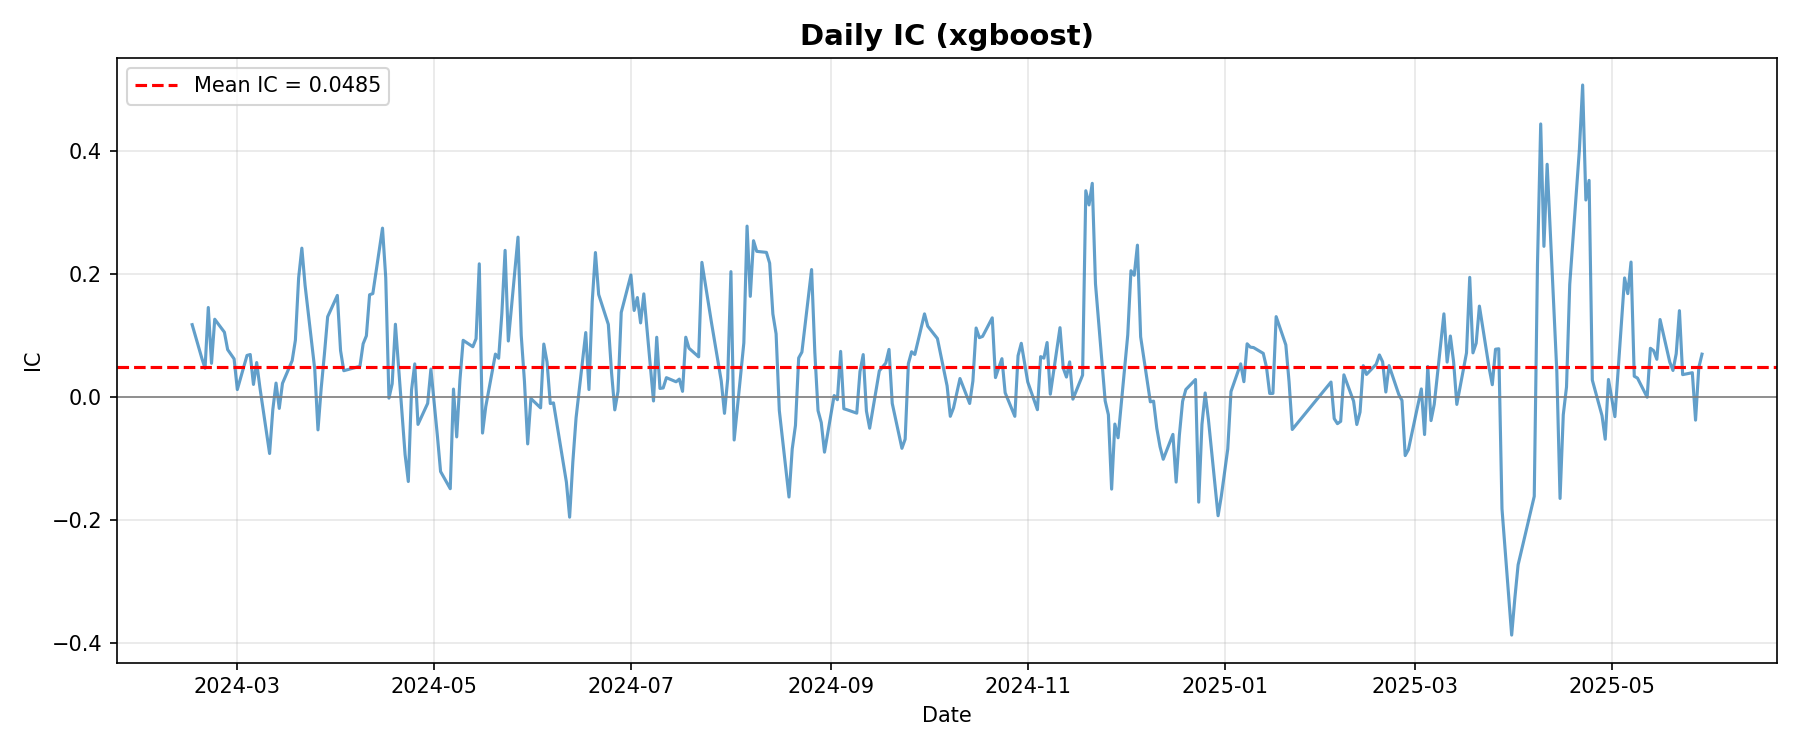
\includegraphics[width=\textwidth]{runs_gpu_static_to_20250601/static/medium/baseline_xgboost/plots/daily_ic.png}
    \caption{XGBoost}
  \end{subfigure}
  \par\vspace{0.5em}
  \begin{subfigure}[t]{0.47\textwidth}
    \centering
    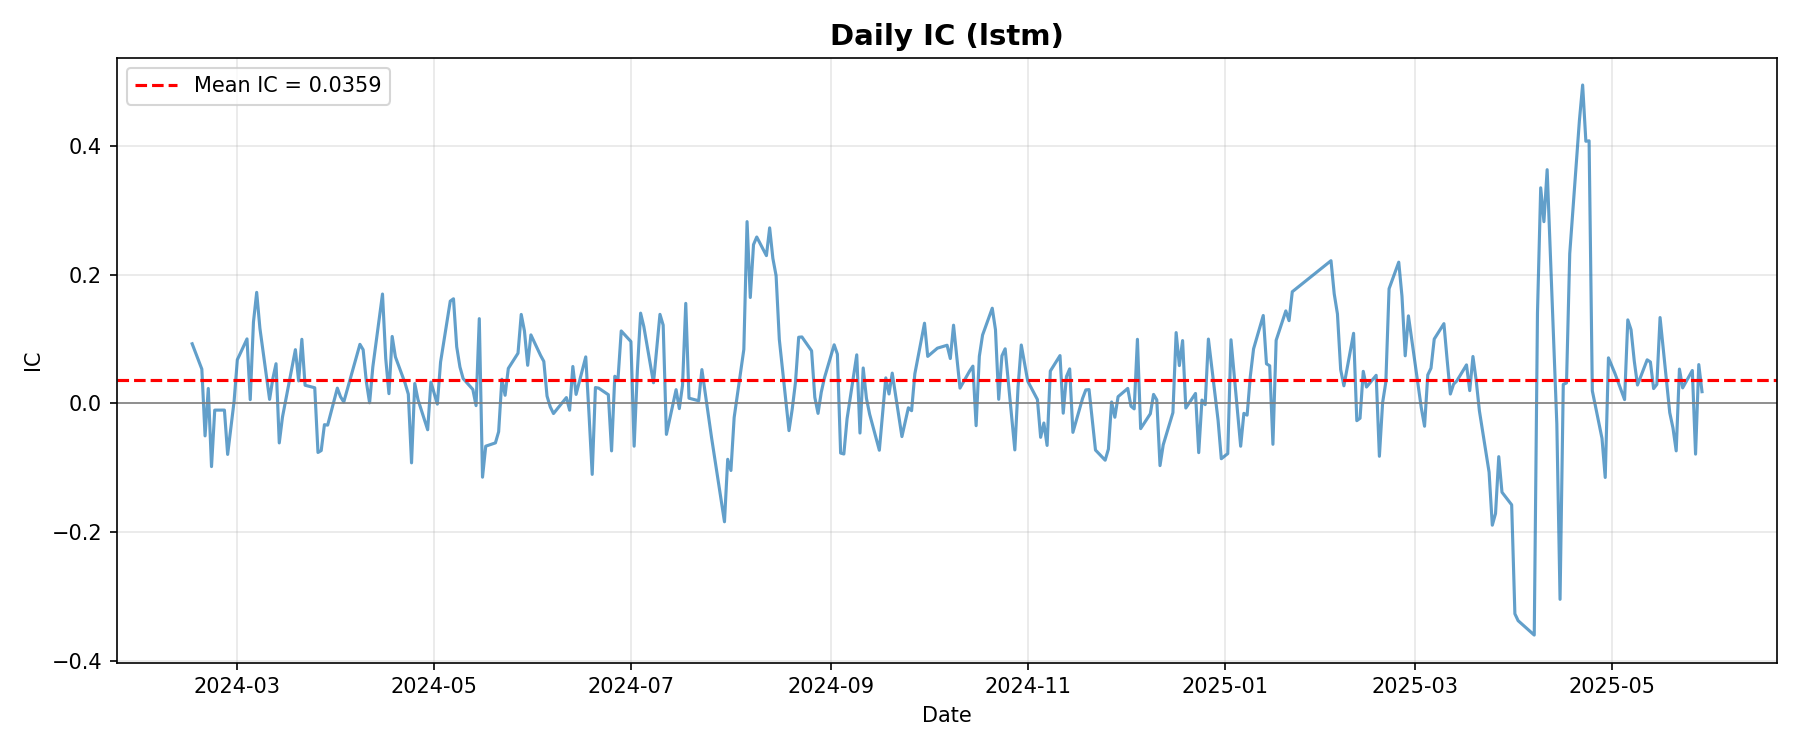
\includegraphics[width=\textwidth]{runs_gpu_static_to_20250601/static/medium/baseline_lstm/plots/daily_ic.png}
    \caption{LSTM}
  \end{subfigure}
  \hfill
  \begin{subfigure}[t]{0.47\textwidth}
    \centering
    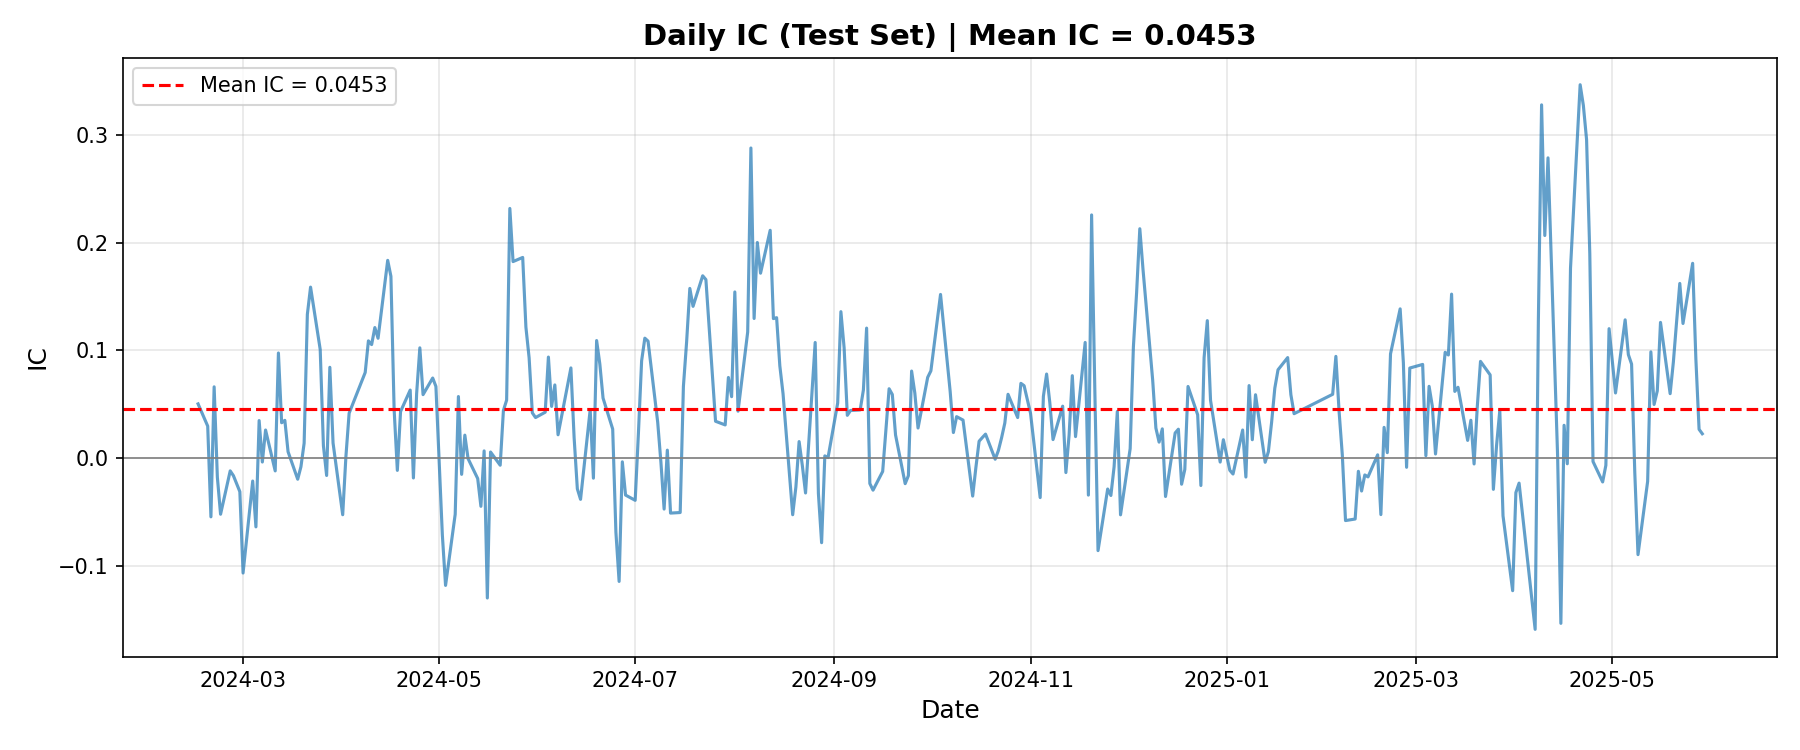
\includegraphics[width=\textwidth]{runs_gpu_static_to_20250601/static/medium/mlp/plots/daily_ic.png}
    \caption{DNN}
  \end{subfigure}
  \par\vspace{0.5em}
  \begin{subfigure}[t]{0.47\textwidth}
    \centering
    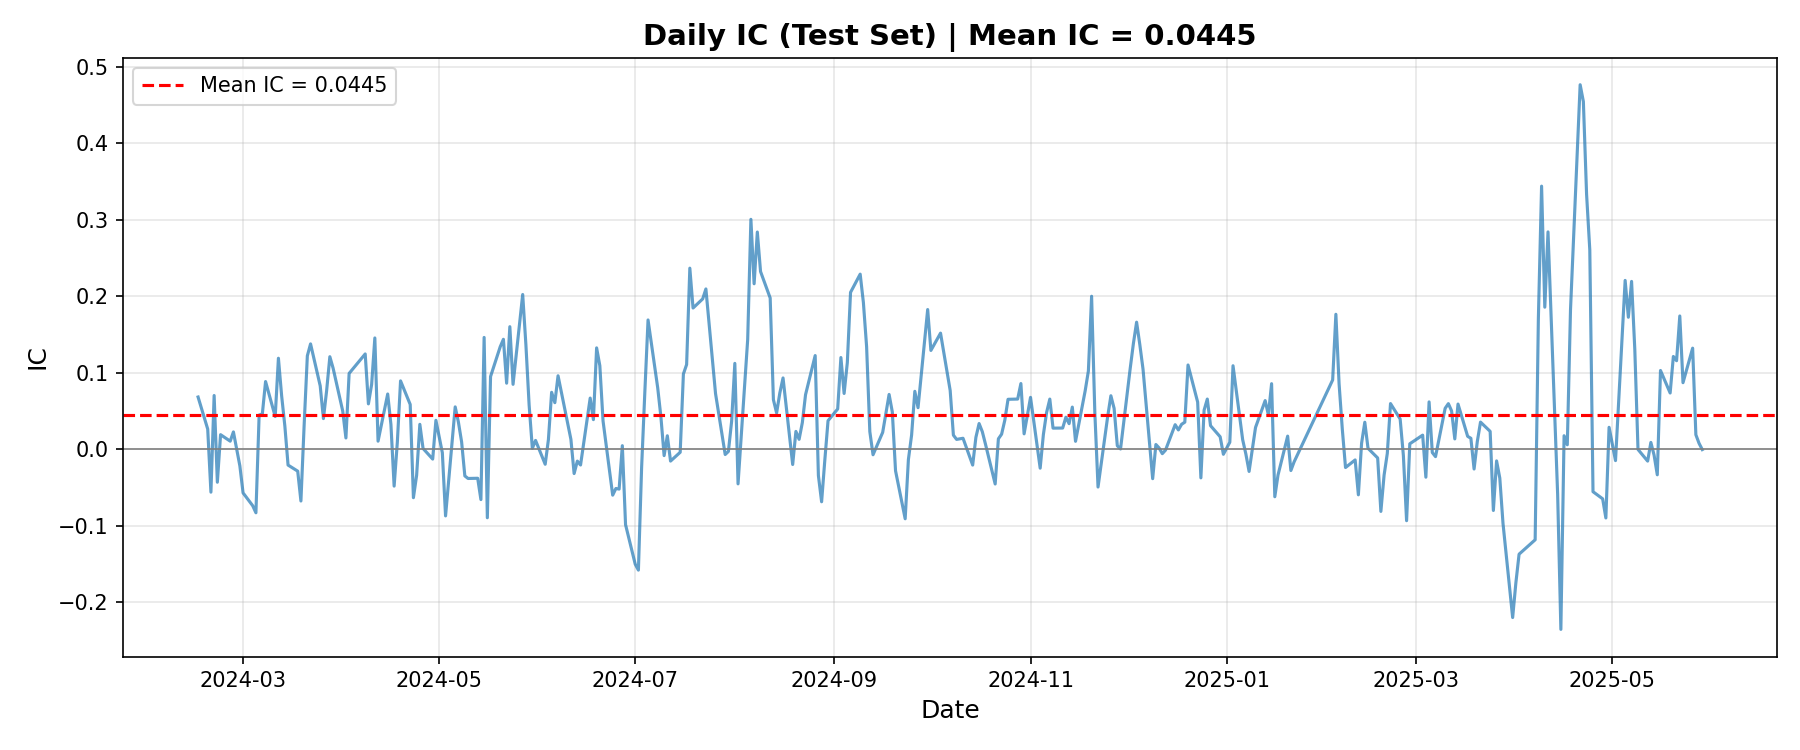
\includegraphics[width=\textwidth]{runs_gpu_static_to_20250601/static/medium/gat_industry/plots/daily_ic.png}
    \caption{GAT-industry}
  \end{subfigure}
  \hfill
  \begin{subfigure}[t]{0.47\textwidth}
    \centering
    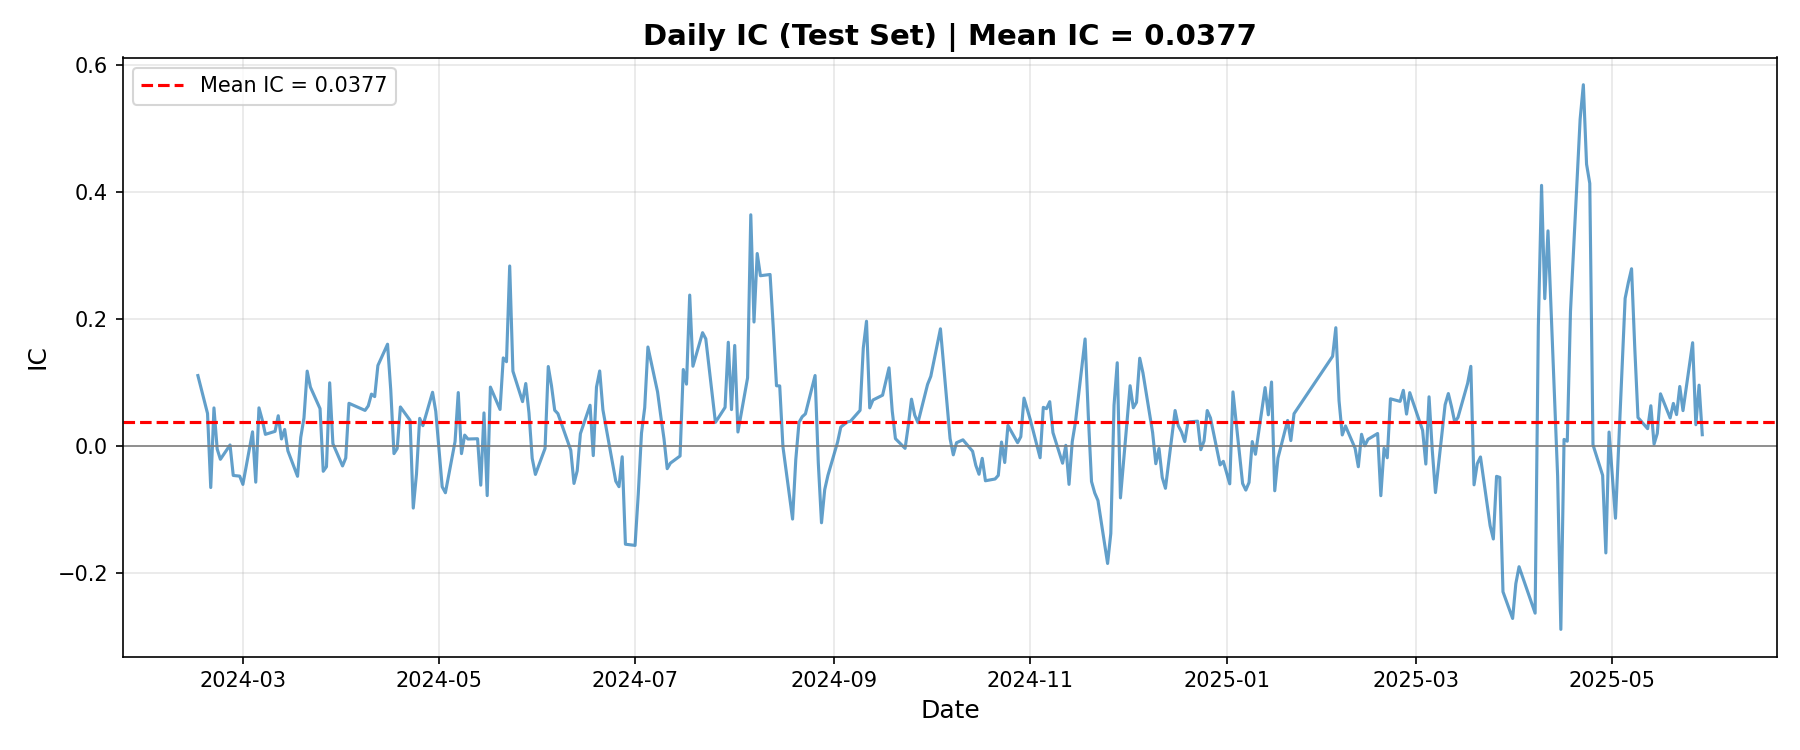
\includegraphics[width=\textwidth]{runs_gpu_static_to_20250601/static/medium/gat_universe/plots/daily_ic.png}
    \caption{GAT-universe}
  \end{subfigure}
  \par\vspace{0.5em}
  \begin{subfigure}[t]{0.47\textwidth}
    \centering
    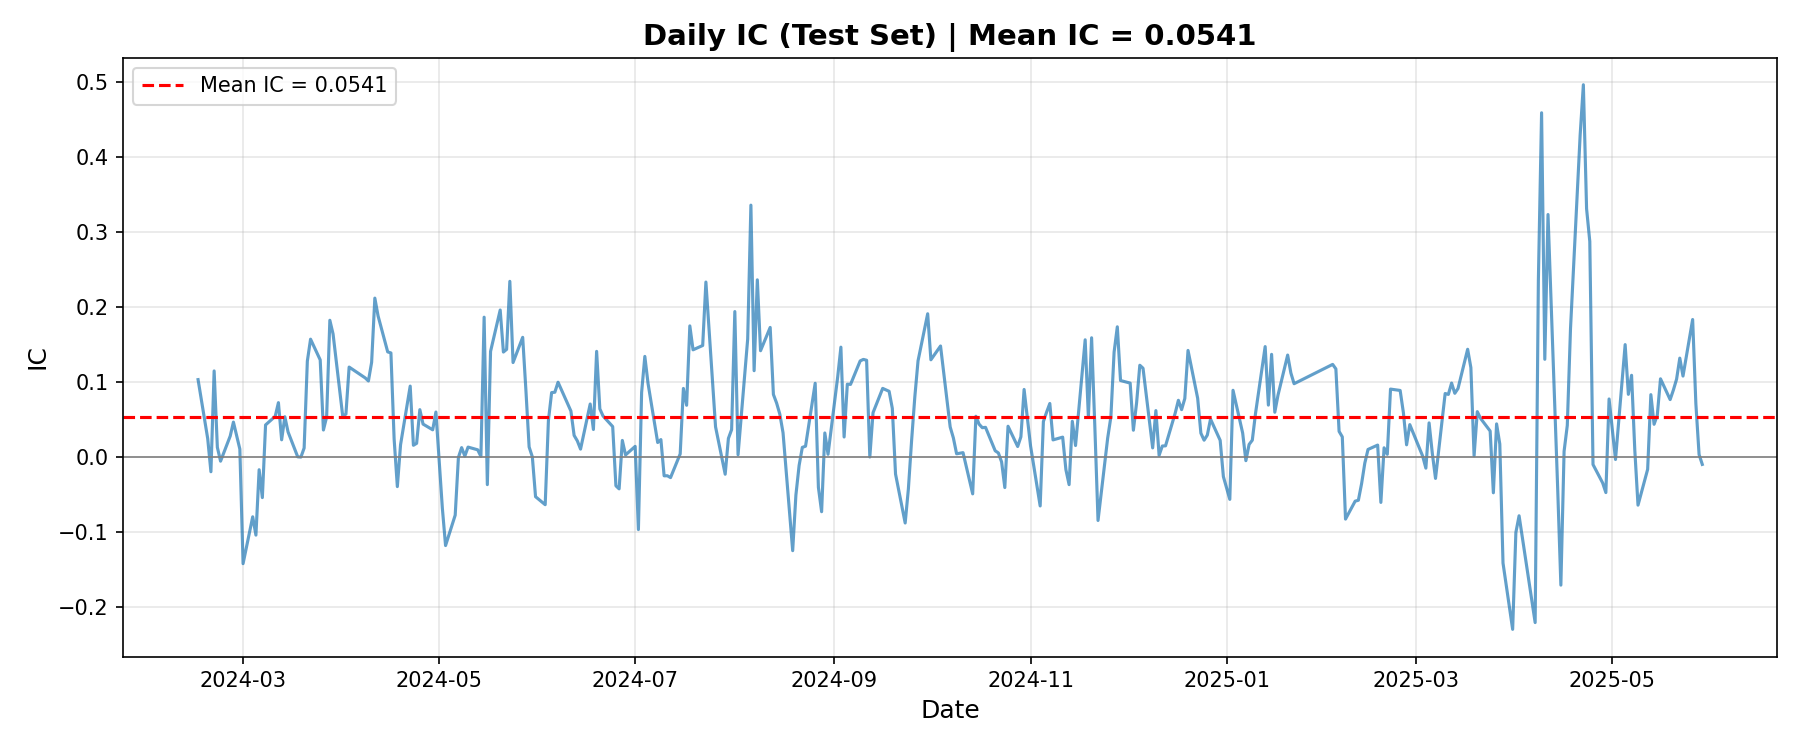
\includegraphics[width=\textwidth]{runs_gpu_static_to_20250601/static/medium/gat_two_graph_no_neutral/plots/daily_ic.png}
    \caption{GAT-TwoGraph}
  \end{subfigure}
  \hfill
  \begin{subfigure}[t]{0.47\textwidth}
    \centering
    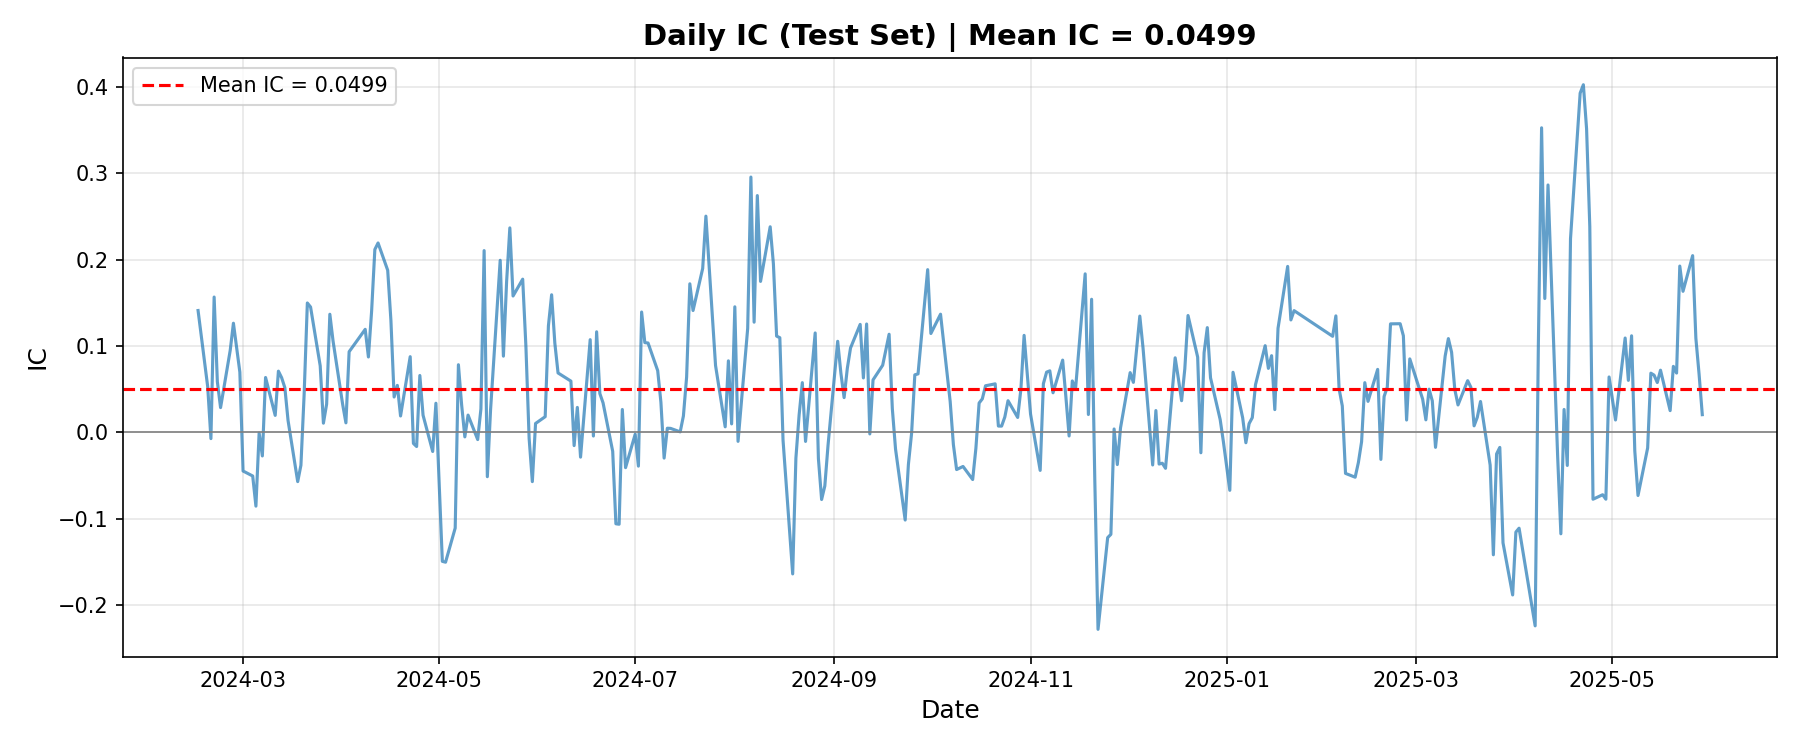
\includegraphics[width=\textwidth]{runs_gpu_static_to_20250601/static/medium/dmfm_ind_neutral/plots/daily_ic.png}
    \caption{GAT-IndNeutral}
  \end{subfigure}
  \par\vspace{0.5em}
  \hfill
  \begin{subfigure}[t]{0.47\textwidth}
    \centering
    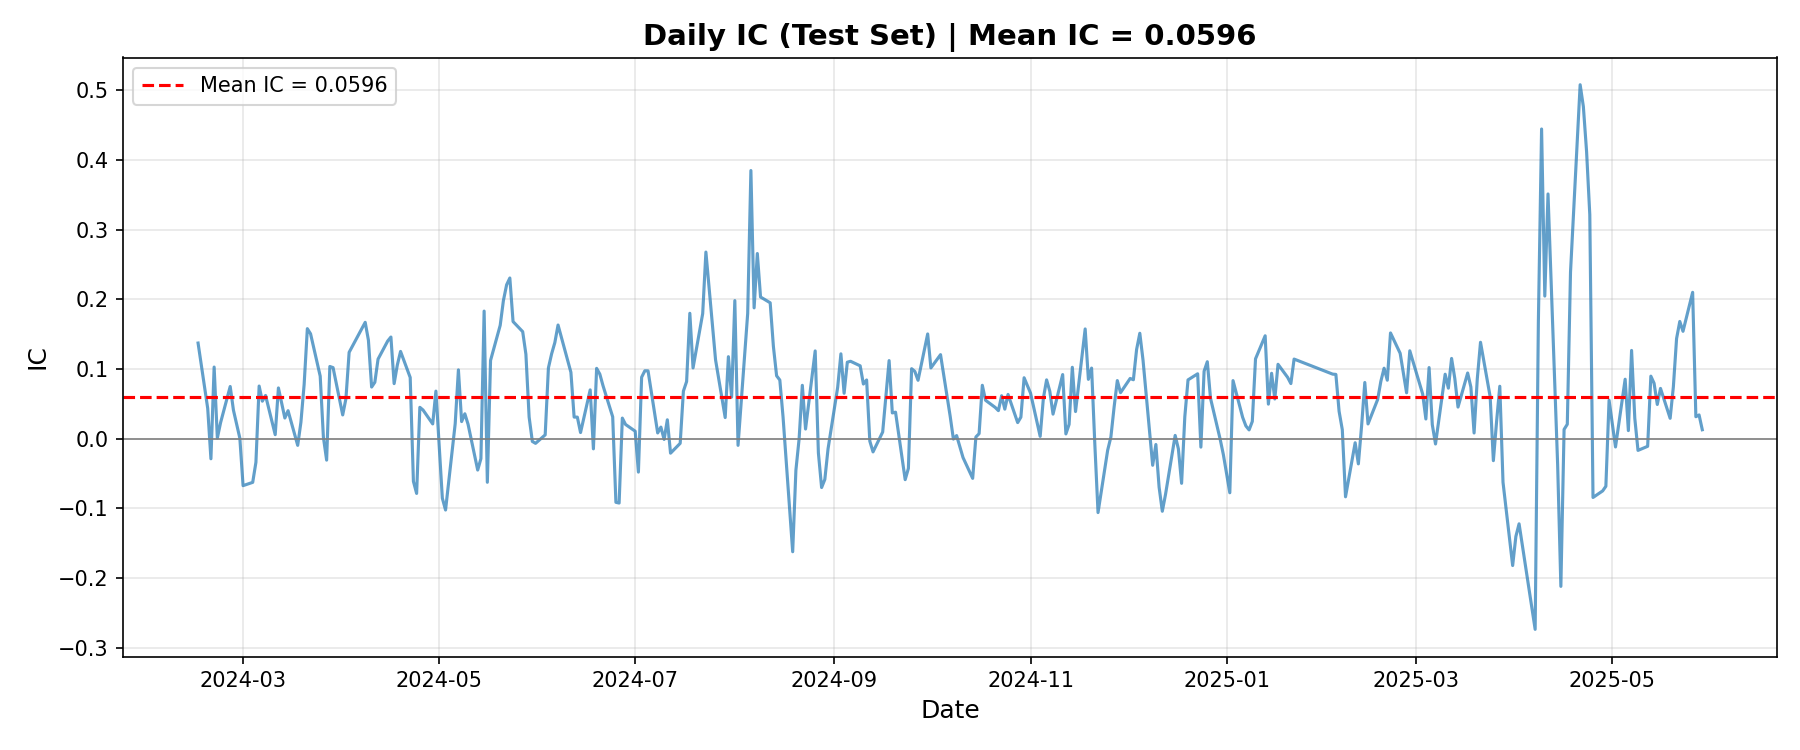
\includegraphics[width=\textwidth]{runs_gpu_static_to_20250601/static/medium/dmfm_full/plots/daily_ic.png}
    \caption{GAT-full}
  \end{subfigure}
  \hfill
  \par\vspace{0.3em}
  \caption{Medium window 各模型 Daily IC 時序。}
  \label{fig:appendix_static_daily_ic_medium}
\end{figure}

\clearpage
\begin{figure}[H]
  \centering
  \captionsetup[subfigure]{font=small}
  \begin{subfigure}[t]{0.47\textwidth}
    \centering
    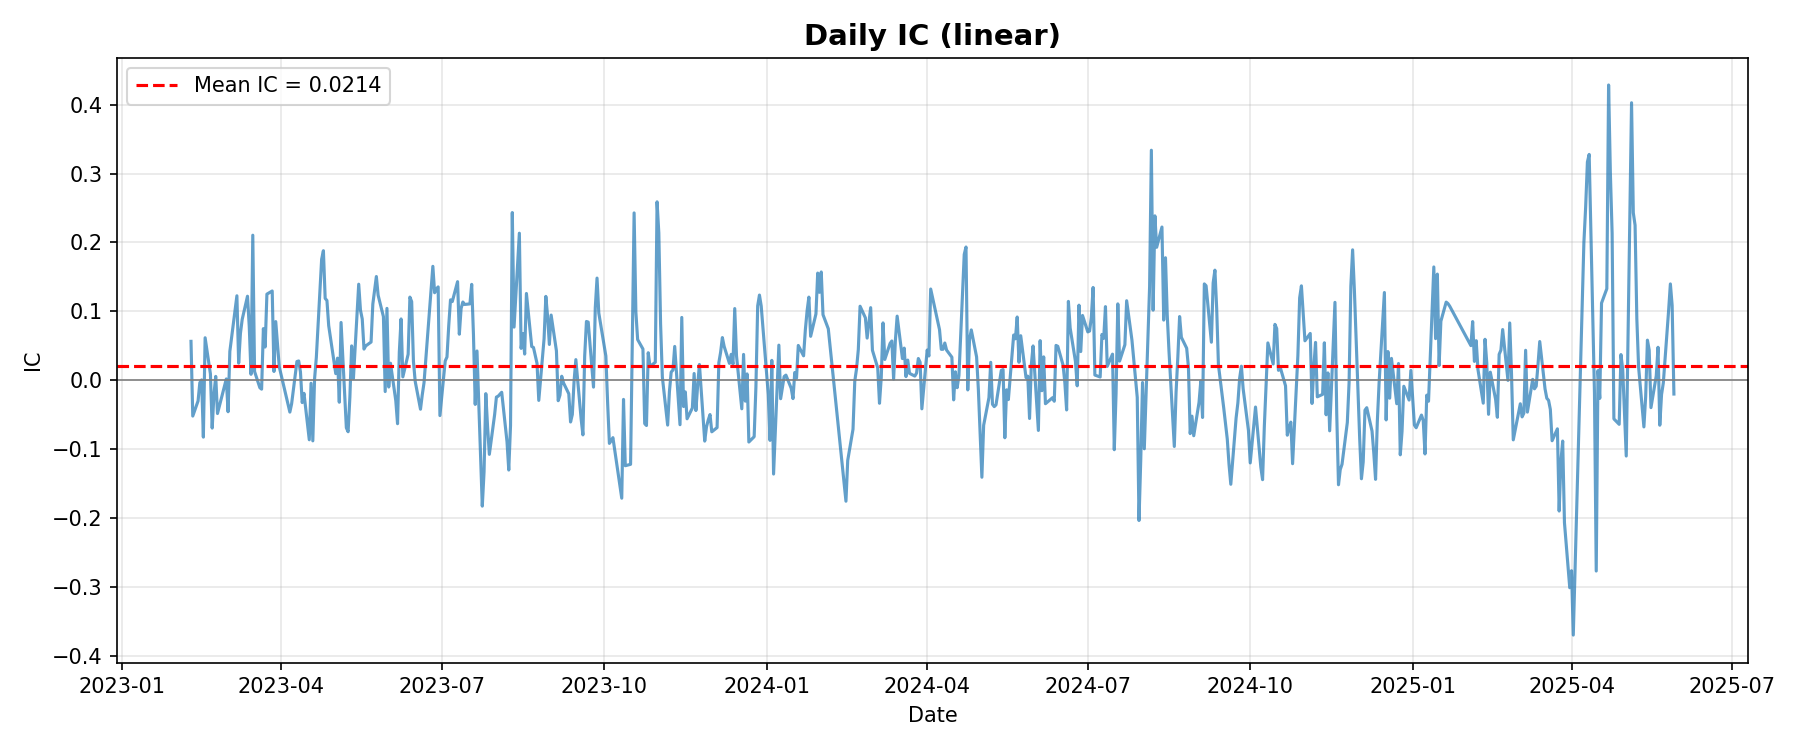
\includegraphics[width=\textwidth]{runs_gpu_static_to_20250601/static/long/baseline_linear/plots/daily_ic.png}
    \caption{Linear}
  \end{subfigure}
  \hfill
  \begin{subfigure}[t]{0.47\textwidth}
    \centering
    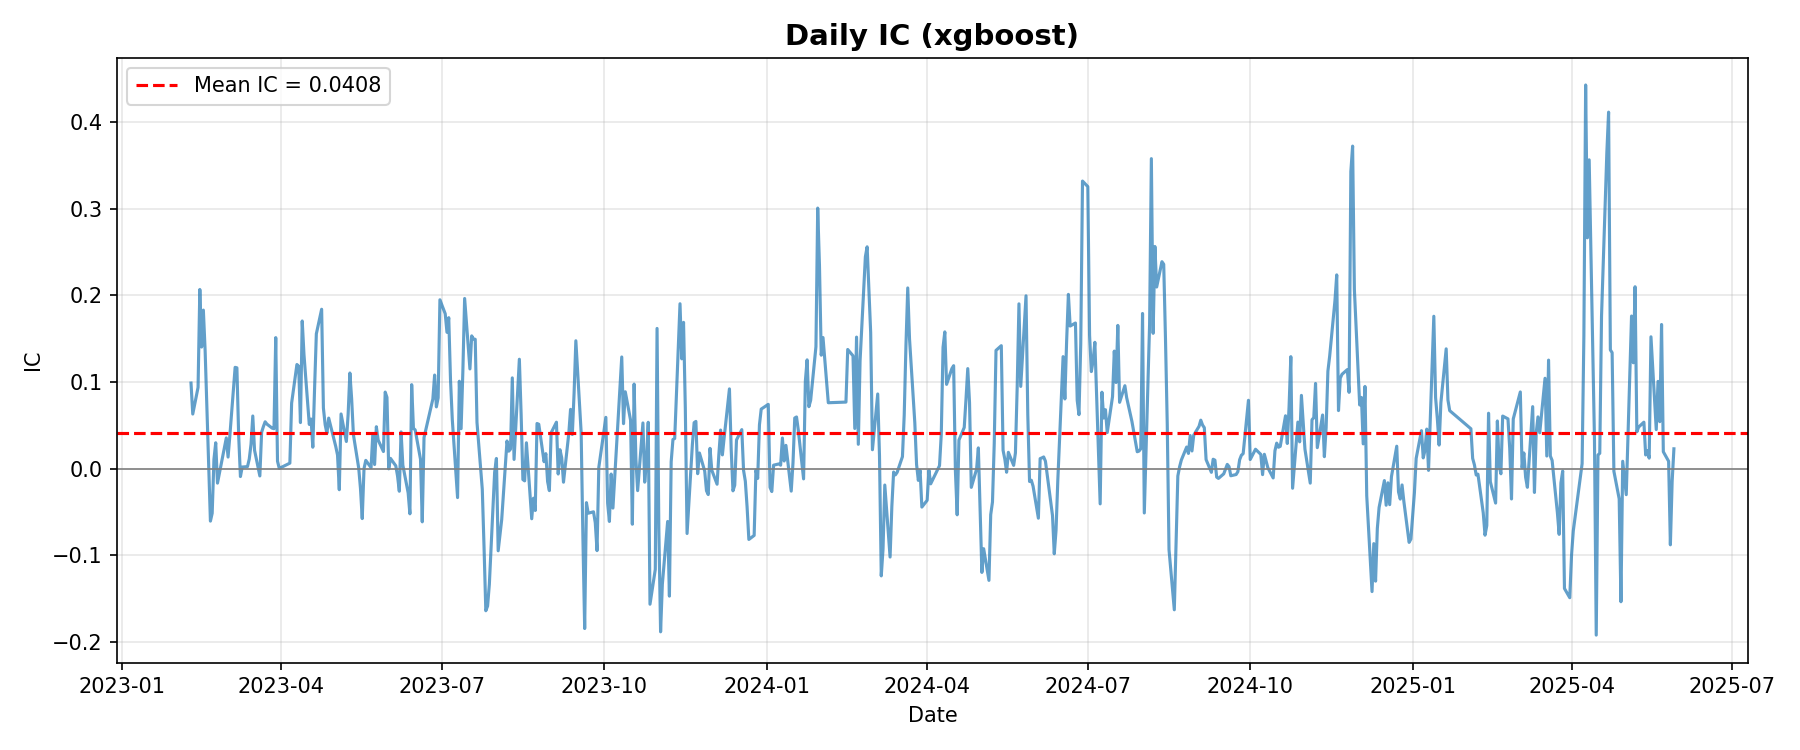
\includegraphics[width=\textwidth]{runs_gpu_static_to_20250601/static/long/baseline_xgboost/plots/daily_ic.png}
    \caption{XGBoost}
  \end{subfigure}
  \par\vspace{0.5em}
  \begin{subfigure}[t]{0.47\textwidth}
    \centering
    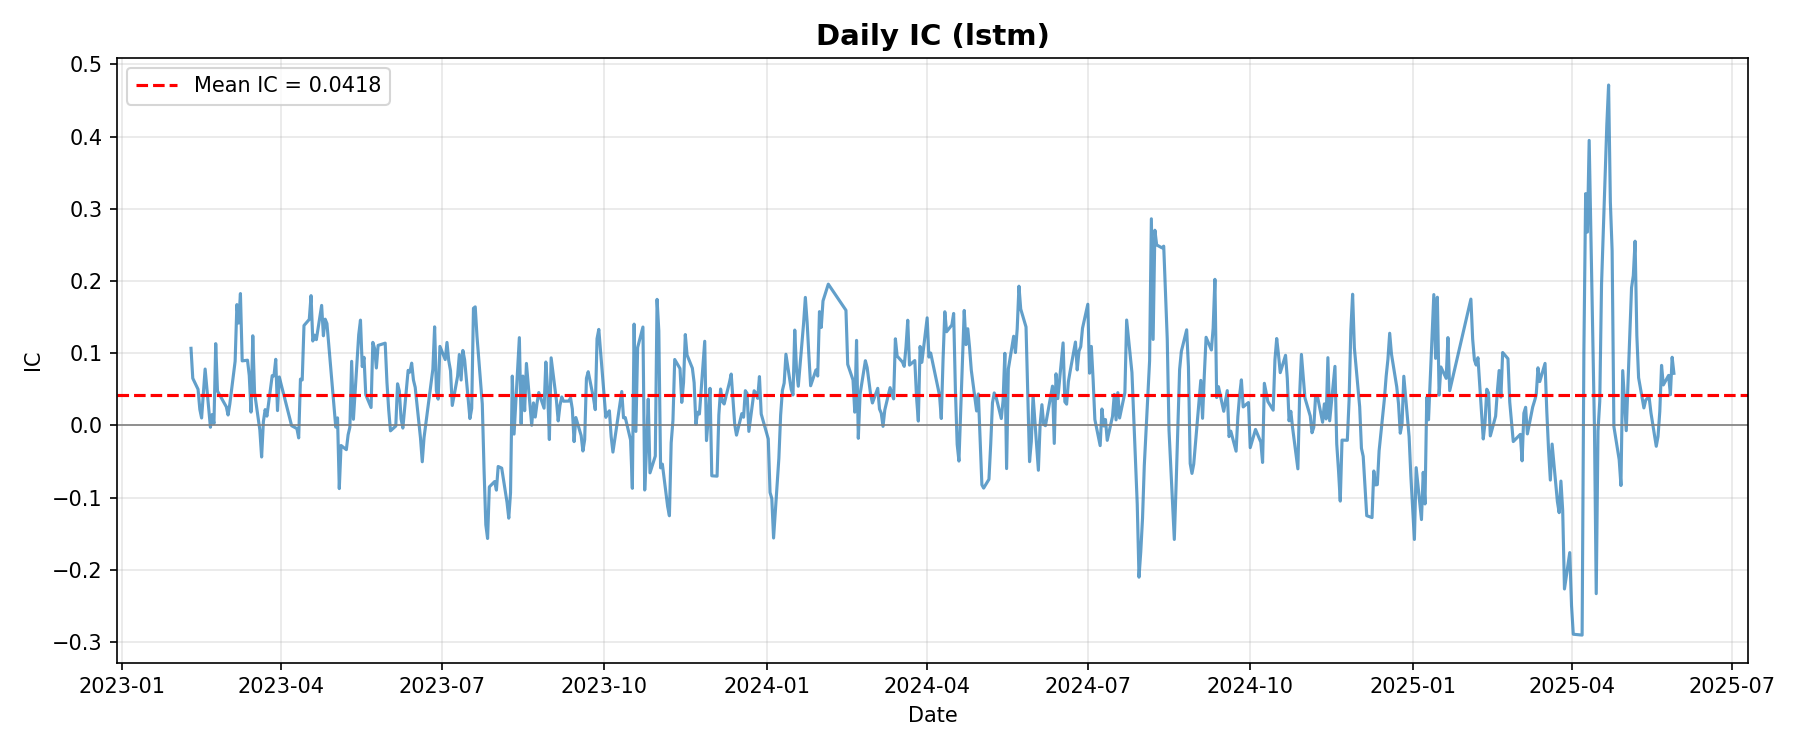
\includegraphics[width=\textwidth]{runs_gpu_static_to_20250601/static/long/baseline_lstm/plots/daily_ic.png}
    \caption{LSTM}
  \end{subfigure}
  \hfill
  \begin{subfigure}[t]{0.47\textwidth}
    \centering
    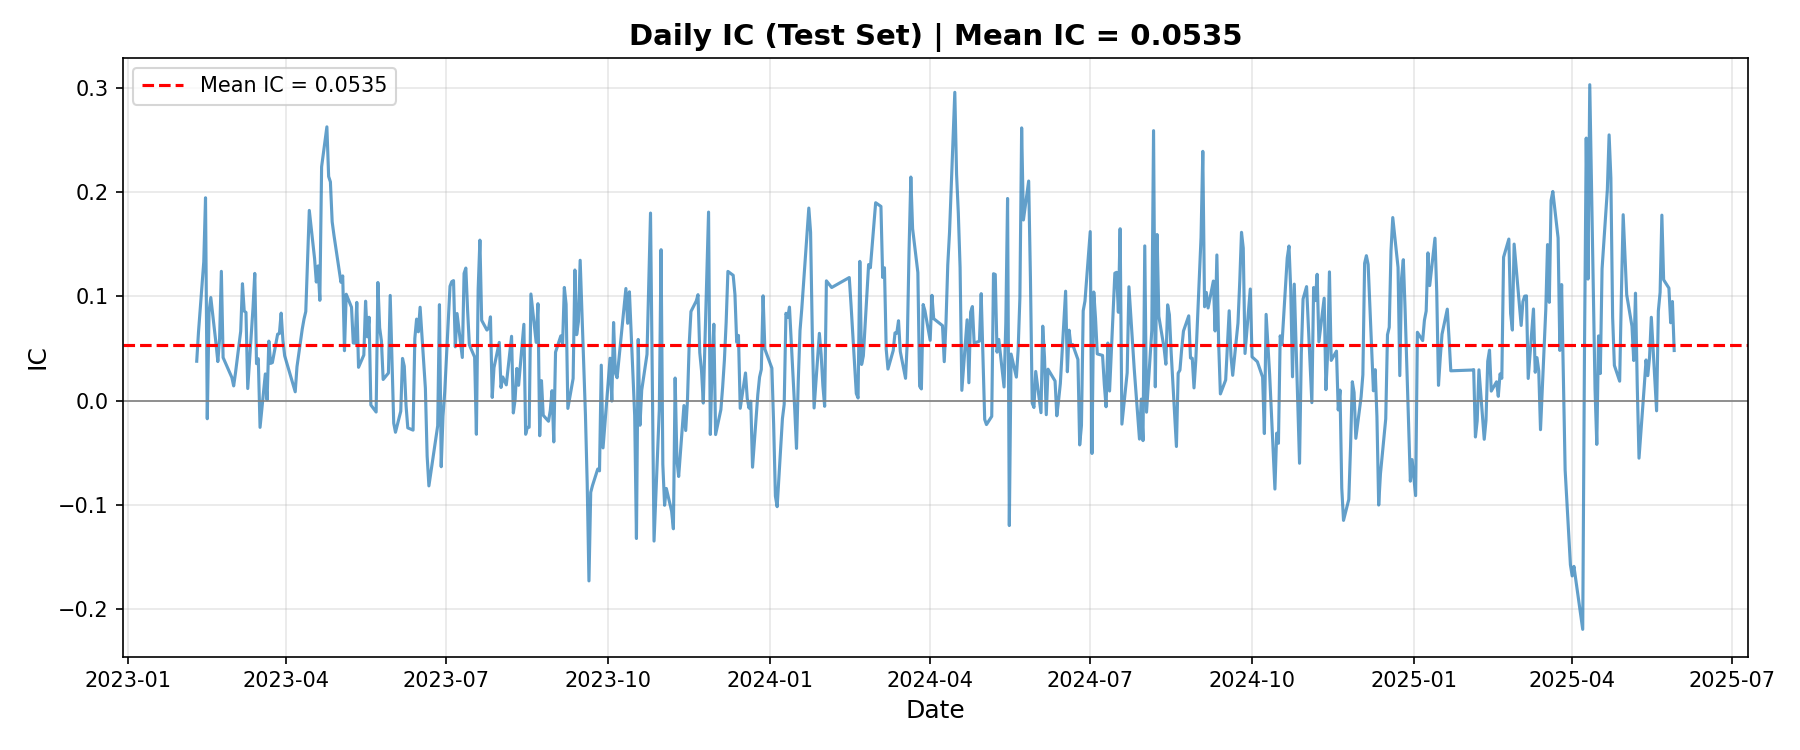
\includegraphics[width=\textwidth]{runs_gpu_static_to_20250601/static/long/mlp/plots/daily_ic.png}
    \caption{DNN}
  \end{subfigure}
  \par\vspace{0.5em}
  \begin{subfigure}[t]{0.47\textwidth}
    \centering
    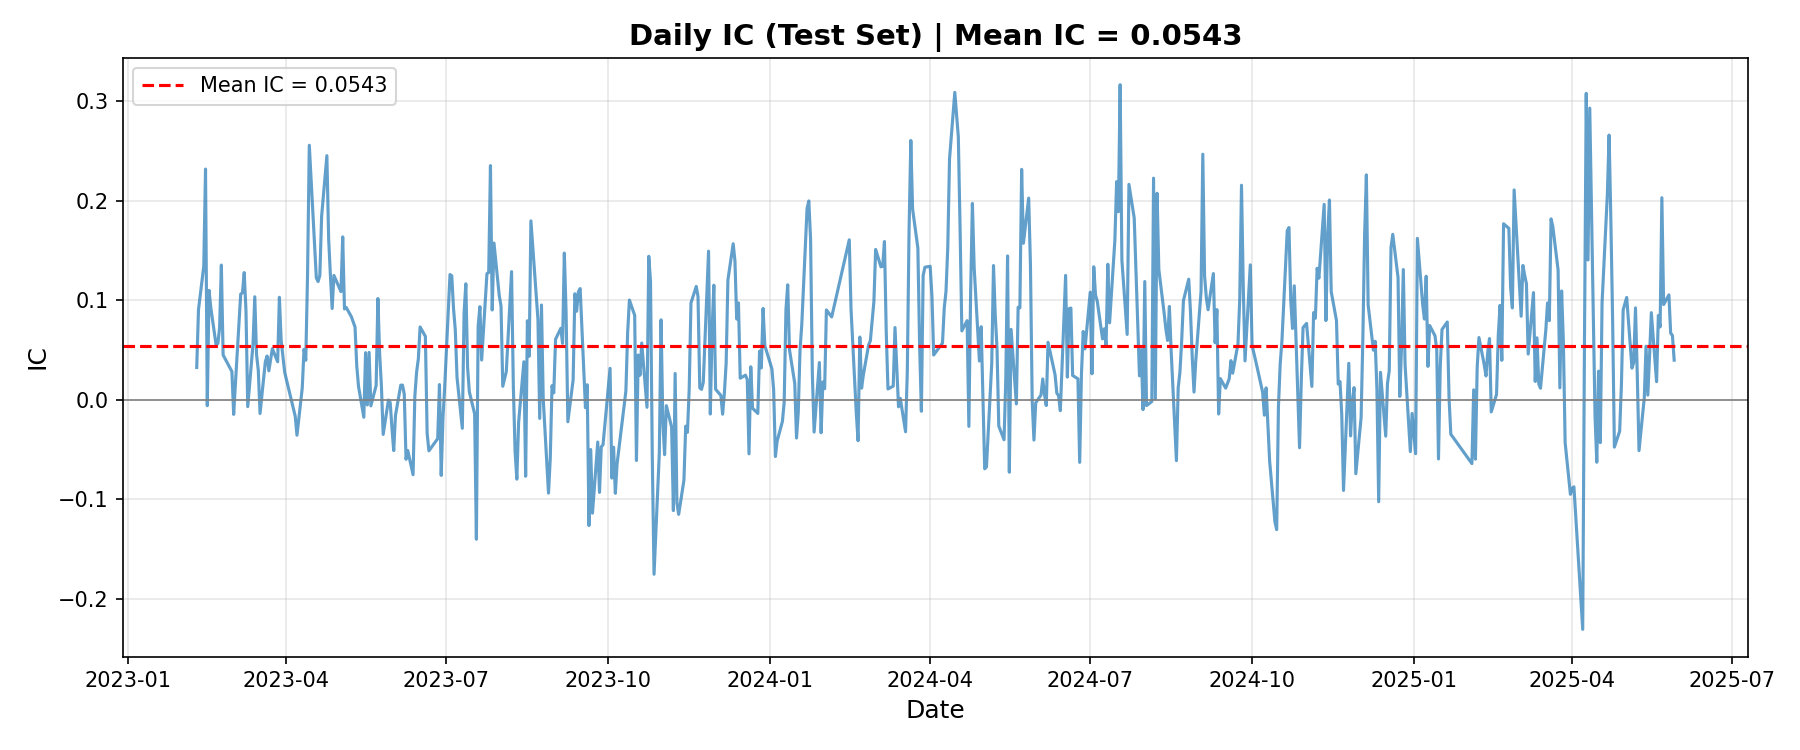
\includegraphics[width=\textwidth]{runs_gpu_static_to_20250601/static/long/gat_industry/plots/daily_ic.png}
    \caption{GAT-industry}
  \end{subfigure}
  \hfill
  \begin{subfigure}[t]{0.47\textwidth}
    \centering
    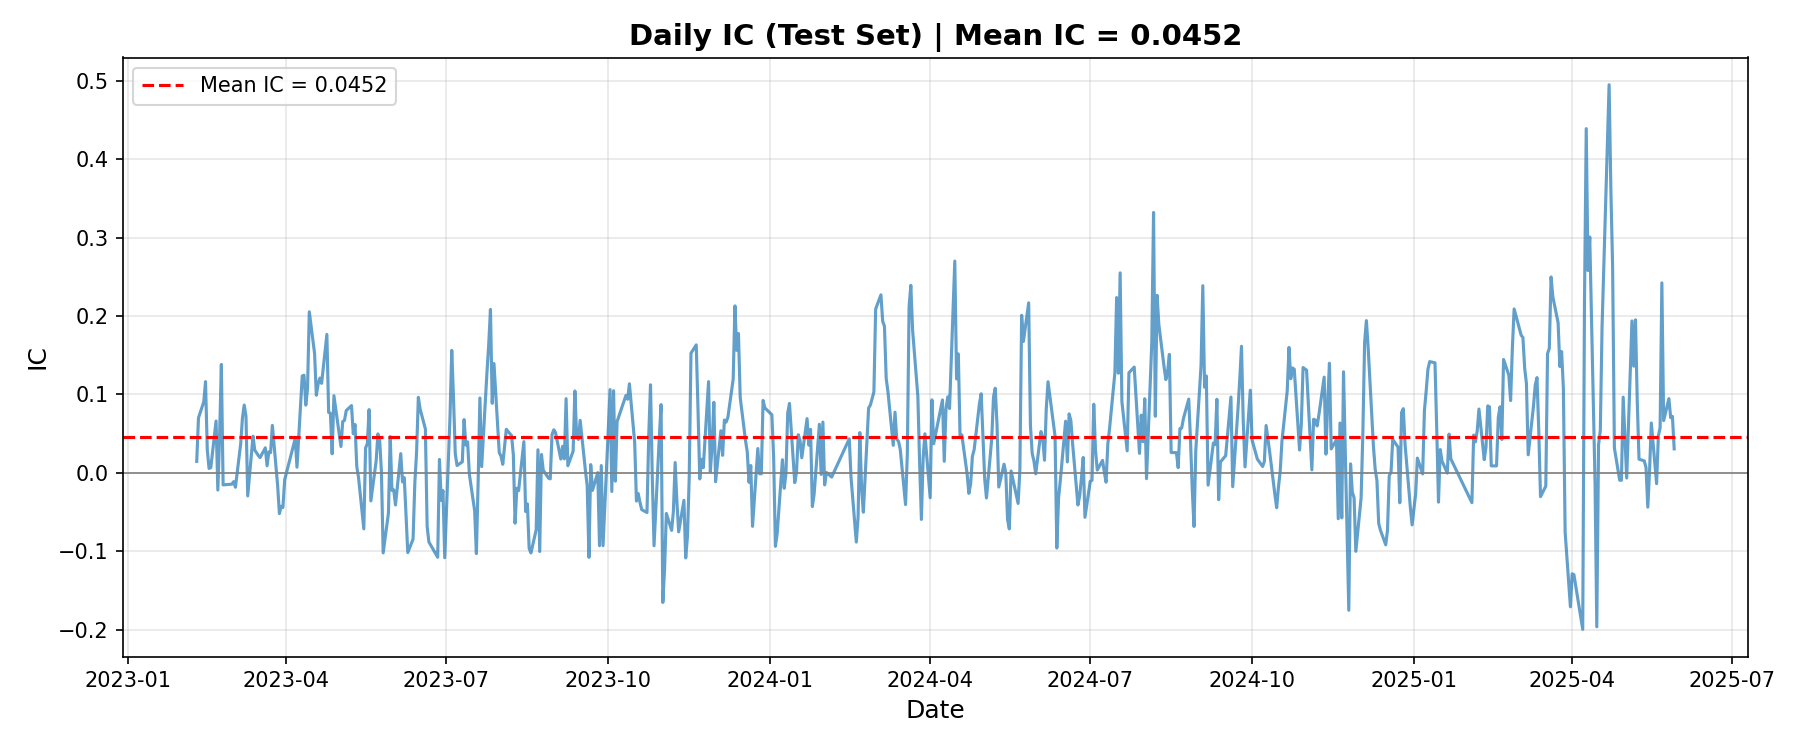
\includegraphics[width=\textwidth]{runs_gpu_static_to_20250601/static/long/gat_universe/plots/daily_ic.png}
    \caption{GAT-universe}
  \end{subfigure}
  \par\vspace{0.5em}
  \begin{subfigure}[t]{0.47\textwidth}
    \centering
    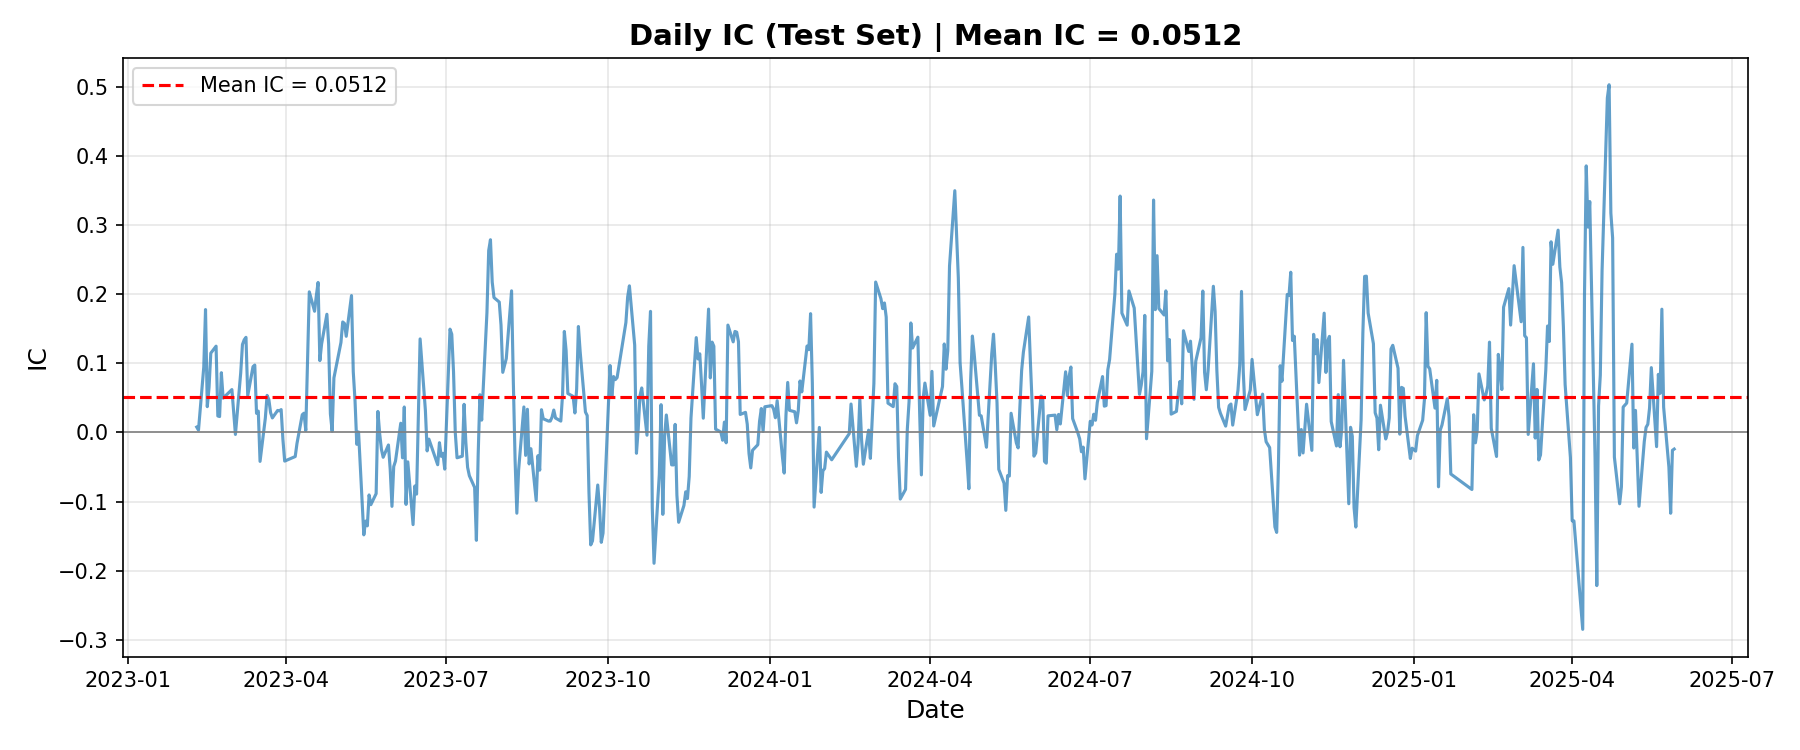
\includegraphics[width=\textwidth]{runs_gpu_static_to_20250601/static/long/gat_two_graph_no_neutral/plots/daily_ic.png}
    \caption{GAT-TwoGraph}
  \end{subfigure}
  \hfill
  \begin{subfigure}[t]{0.47\textwidth}
    \centering
    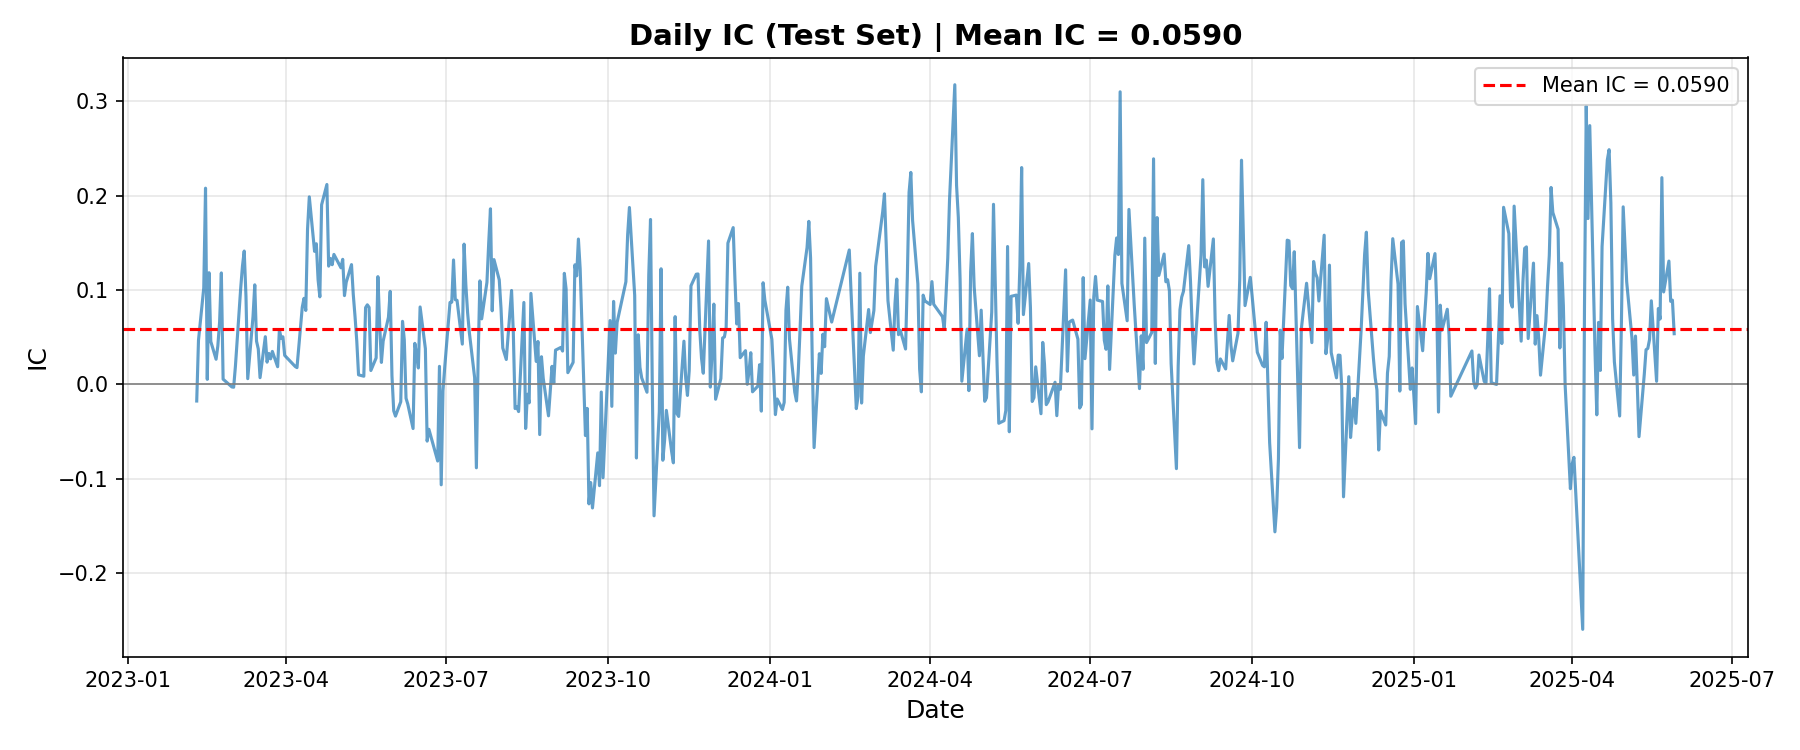
\includegraphics[width=\textwidth]{runs_gpu_static_to_20250601/static/long/dmfm_ind_neutral/plots/daily_ic.png}
    \caption{GAT-IndNeutral}
  \end{subfigure}
  \par\vspace{0.5em}
  \hfill
  \begin{subfigure}[t]{0.47\textwidth}
    \centering
    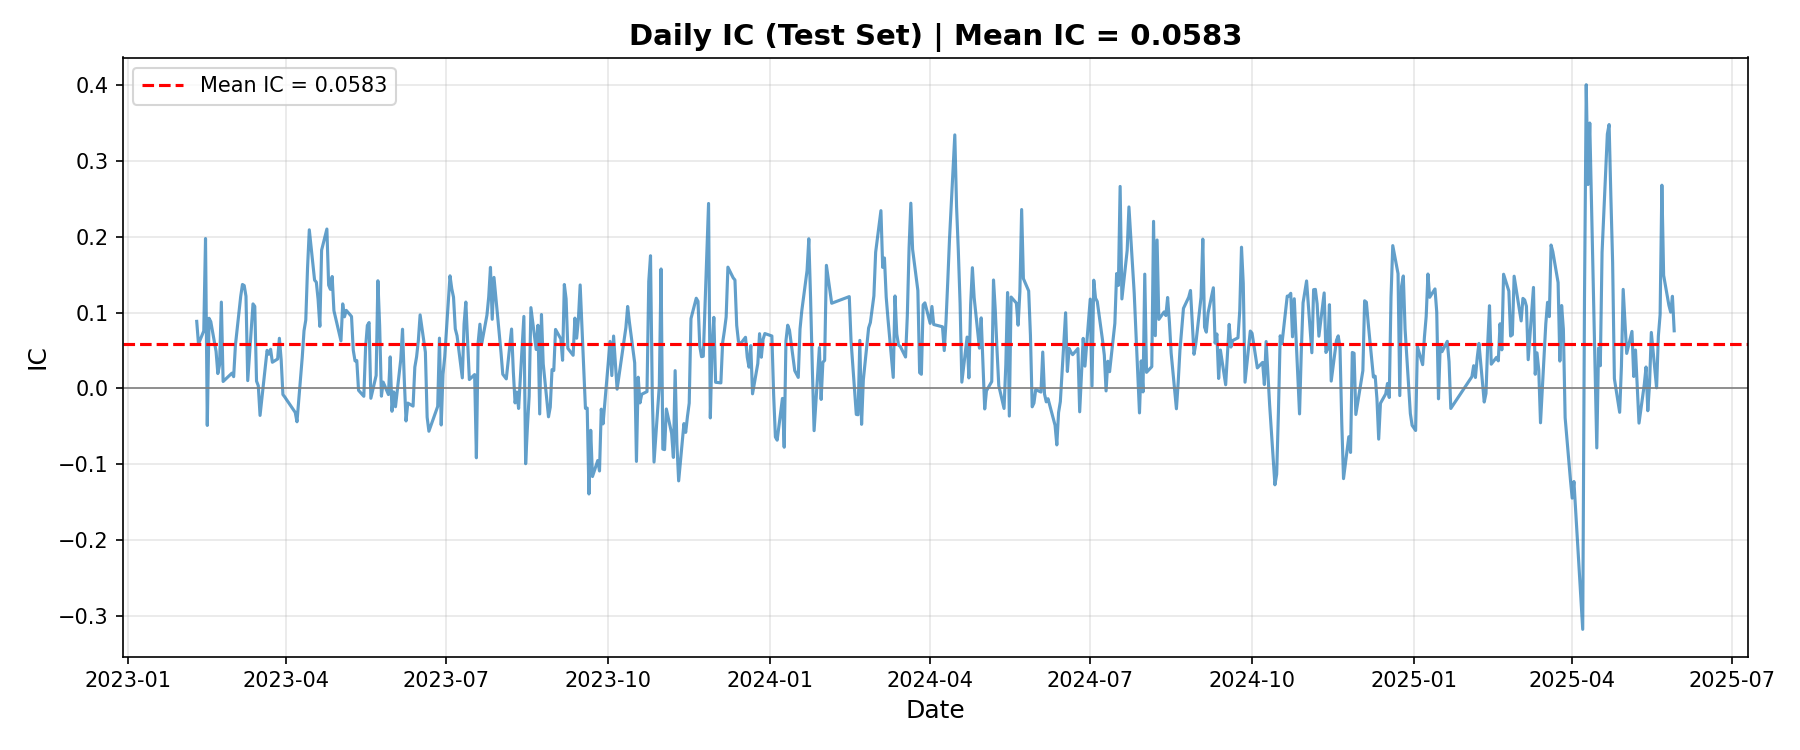
\includegraphics[width=\textwidth]{runs_gpu_static_to_20250601/static/long/dmfm_full/plots/daily_ic.png}
    \caption{GAT-full}
  \end{subfigure}
  \hfill
  \par\vspace{0.3em}
  \caption{Long window 各模型 Daily IC 時序。}
  \label{fig:appendix_static_daily_ic_long}
\end{figure}

\clearpage
\subsection{IC 分佈補充結果}

\begin{figure}[H]
  \centering
  \captionsetup[subfigure]{font=small}
  \begin{subfigure}[t]{0.47\textwidth}
    \centering
    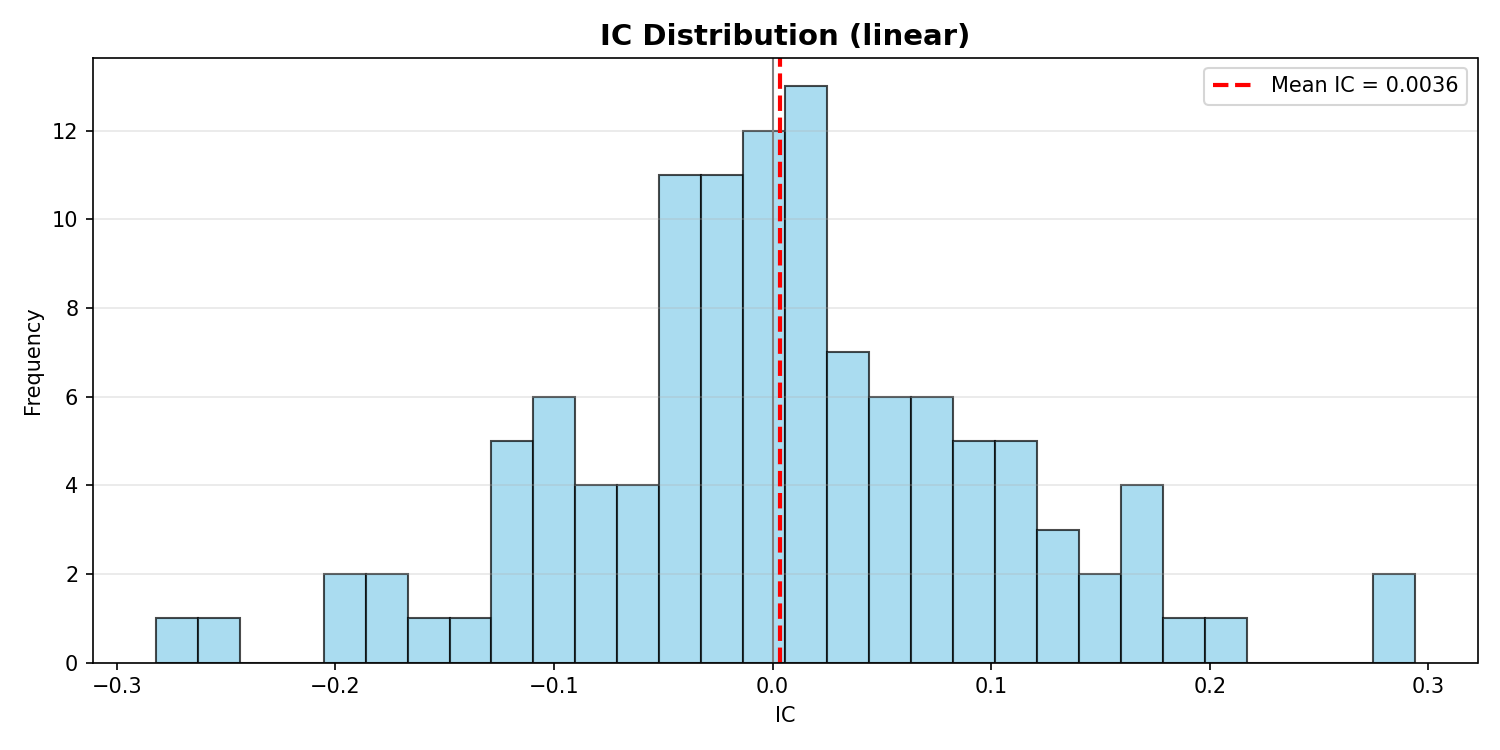
\includegraphics[width=\textwidth]{runs_gpu_static_to_20250601/static/short/baseline_linear/plots/ic_distribution.png}
    \caption{Linear}
  \end{subfigure}
  \hfill
  \begin{subfigure}[t]{0.47\textwidth}
    \centering
    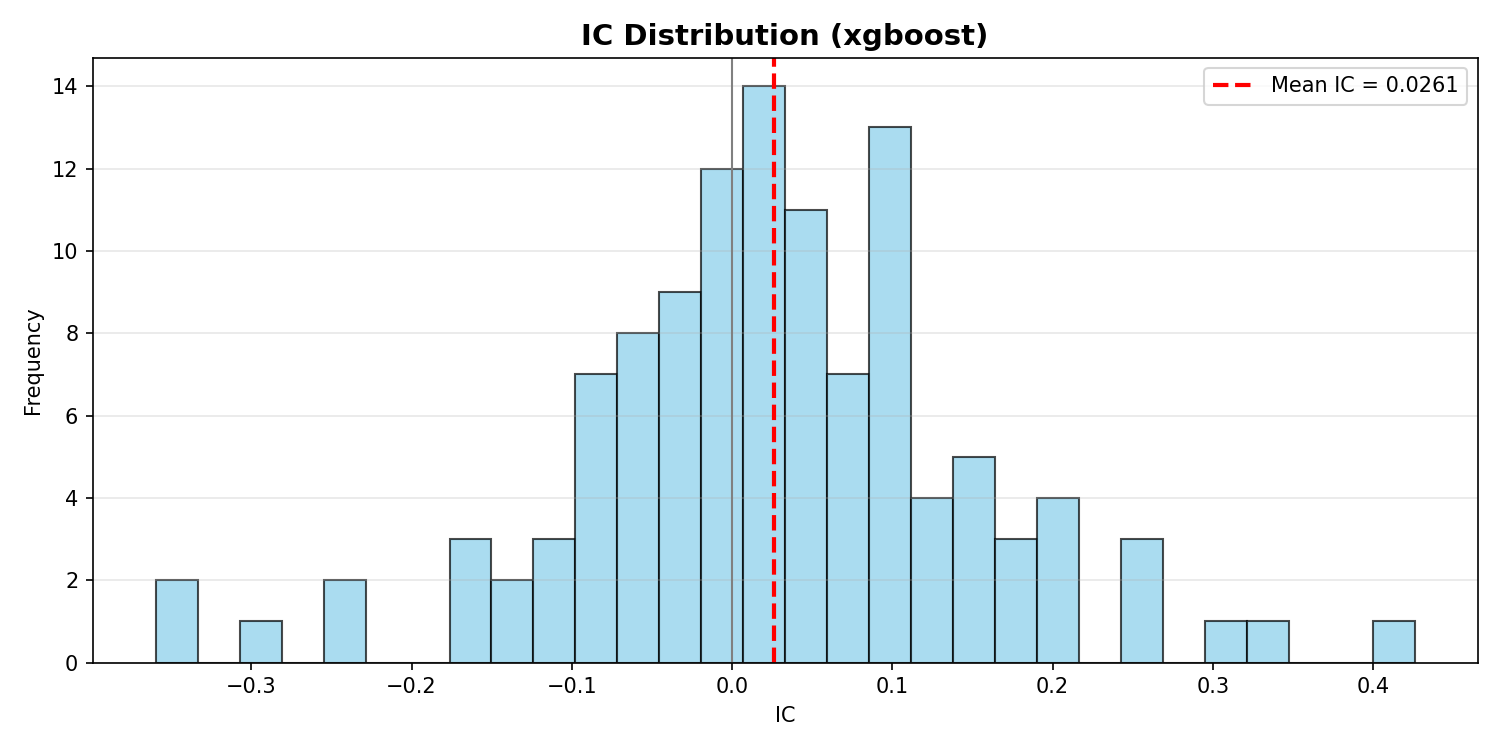
\includegraphics[width=\textwidth]{runs_gpu_static_to_20250601/static/short/baseline_xgboost/plots/ic_distribution.png}
    \caption{XGBoost}
  \end{subfigure}
  \par\vspace{0.5em}
  \begin{subfigure}[t]{0.47\textwidth}
    \centering
    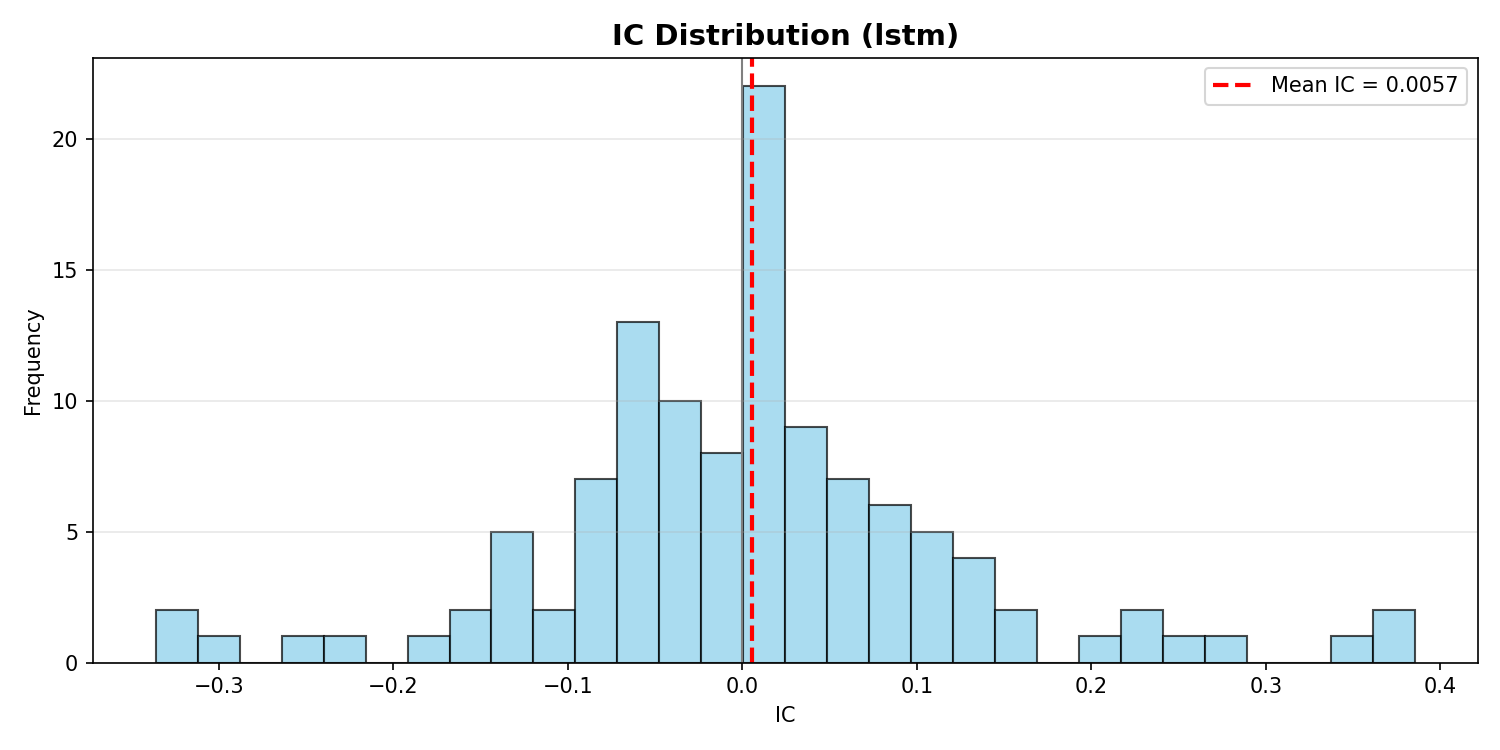
\includegraphics[width=\textwidth]{runs_gpu_static_to_20250601/static/short/baseline_lstm/plots/ic_distribution.png}
    \caption{LSTM}
  \end{subfigure}
  \hfill
  \begin{subfigure}[t]{0.47\textwidth}
    \centering
    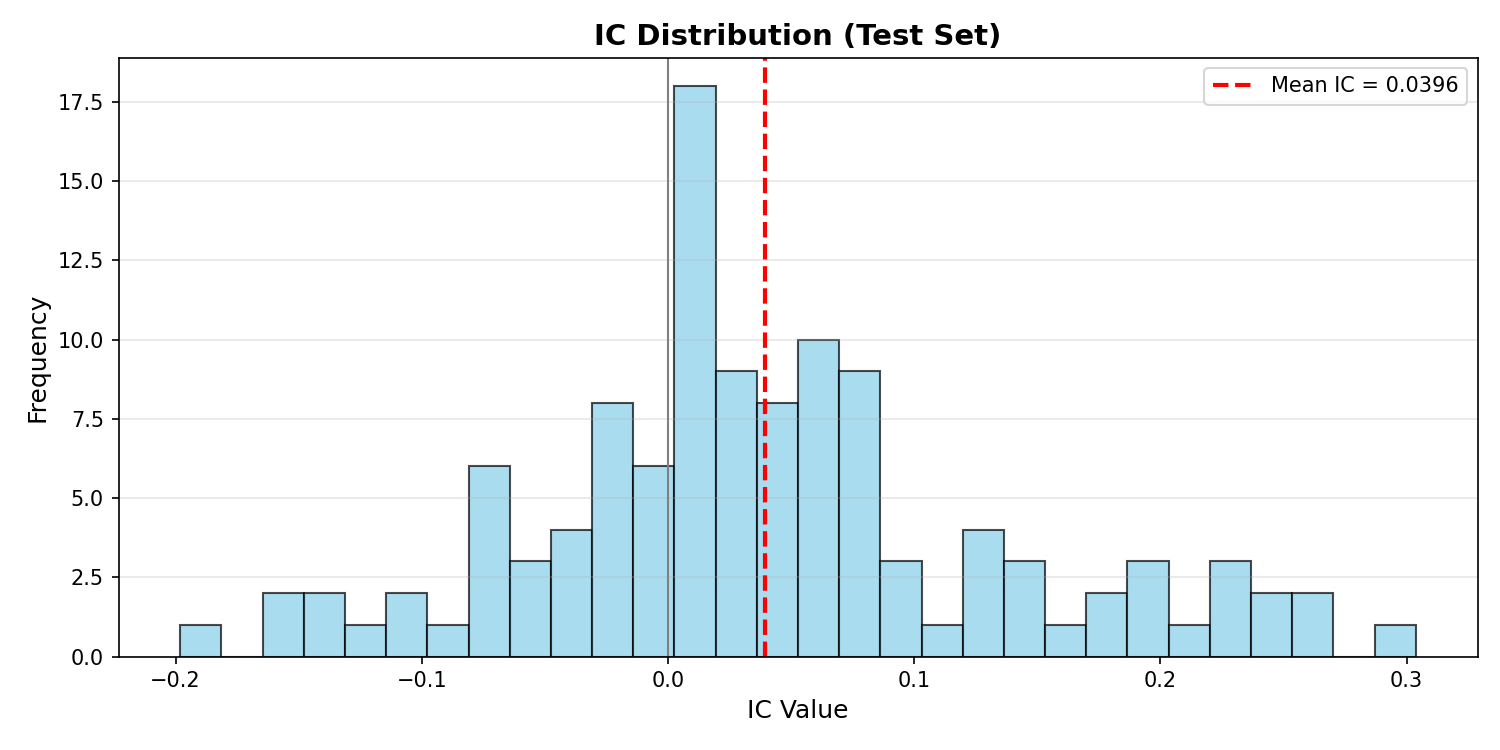
\includegraphics[width=\textwidth]{runs_gpu_static_to_20250601/static/short/mlp/plots/ic_distribution.png}
    \caption{DNN}
  \end{subfigure}
  \par\vspace{0.5em}
  \begin{subfigure}[t]{0.47\textwidth}
    \centering
    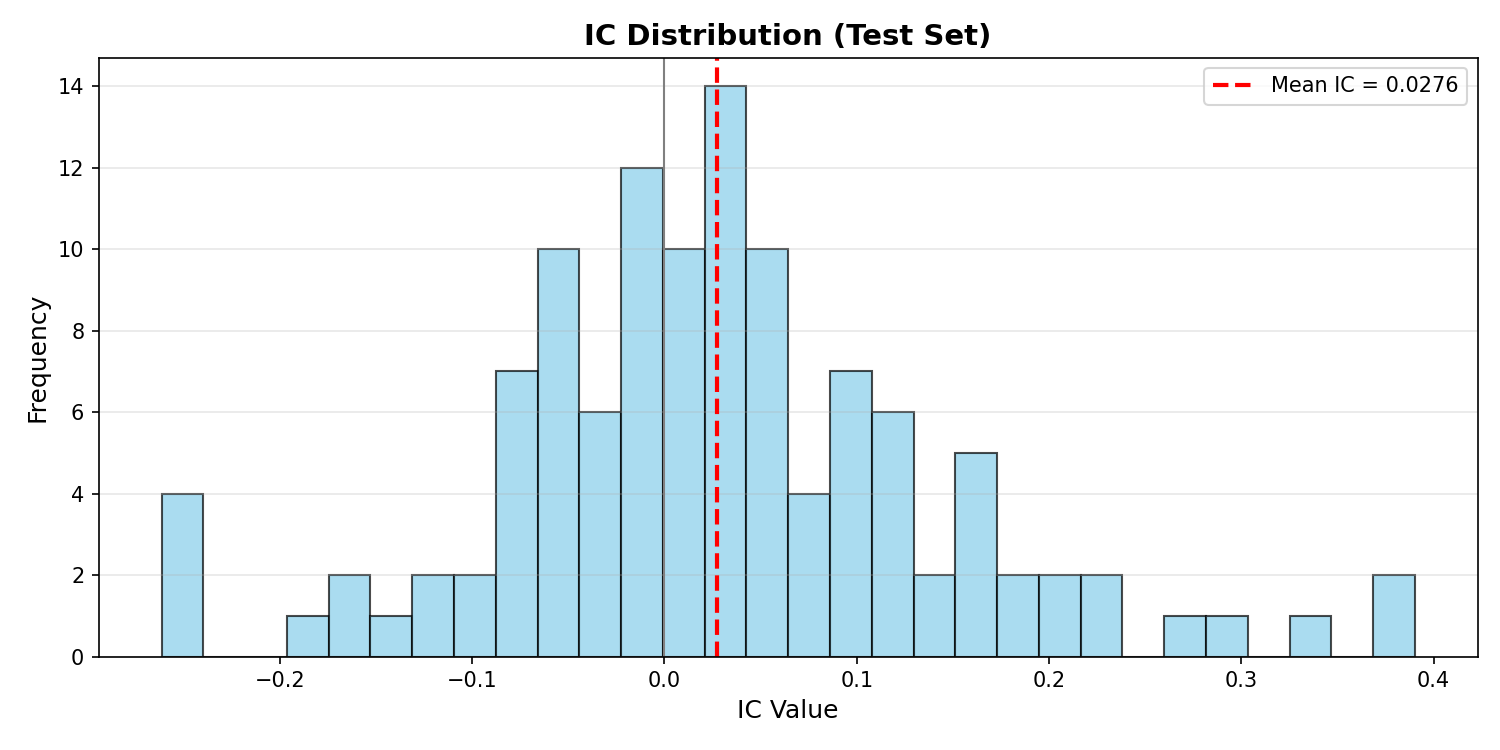
\includegraphics[width=\textwidth]{runs_gpu_static_to_20250601/static/short/gat_industry/plots/ic_distribution.png}
    \caption{GAT-industry}
  \end{subfigure}
  \hfill
  \begin{subfigure}[t]{0.47\textwidth}
    \centering
    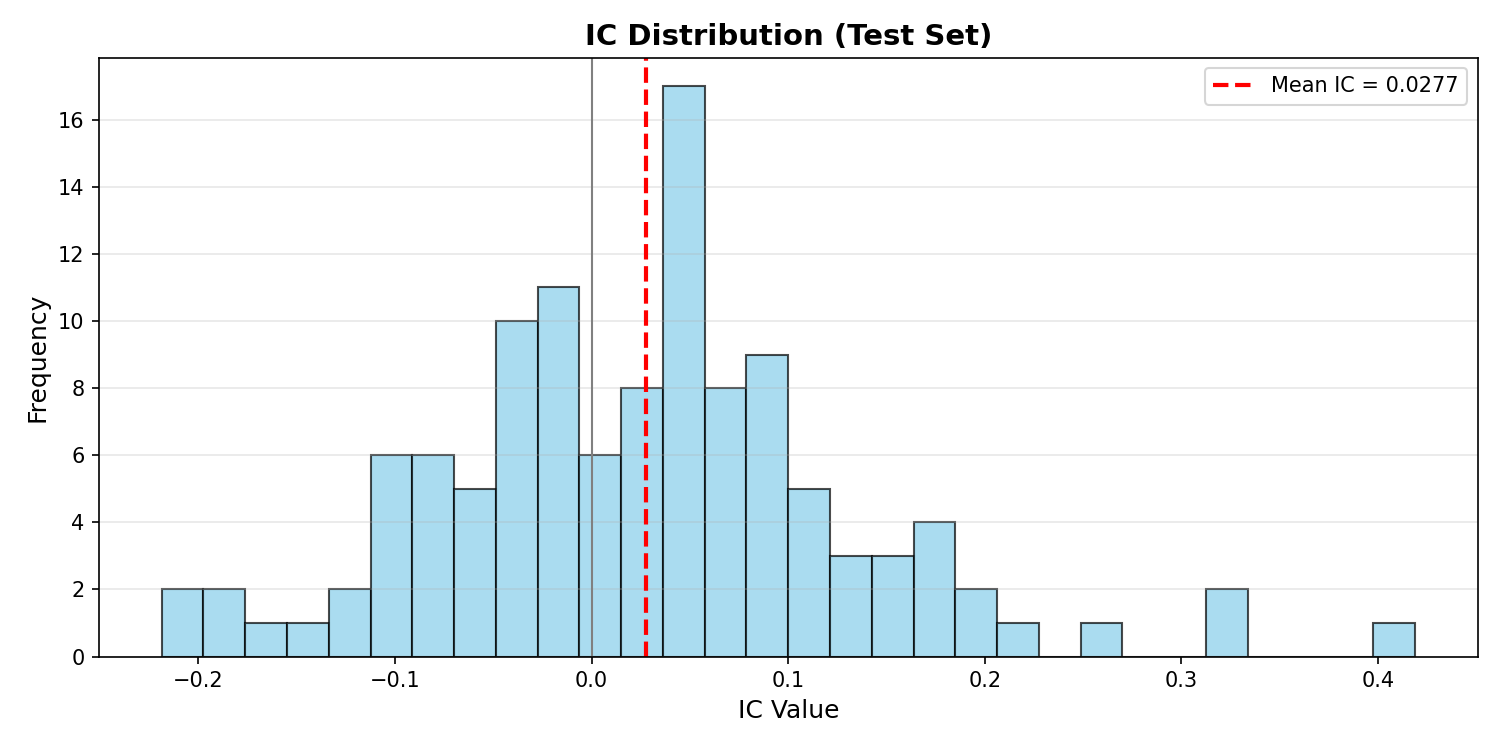
\includegraphics[width=\textwidth]{runs_gpu_static_to_20250601/static/short/gat_universe/plots/ic_distribution.png}
    \caption{GAT-universe}
  \end{subfigure}
  \par\vspace{0.5em}
  \begin{subfigure}[t]{0.47\textwidth}
    \centering
    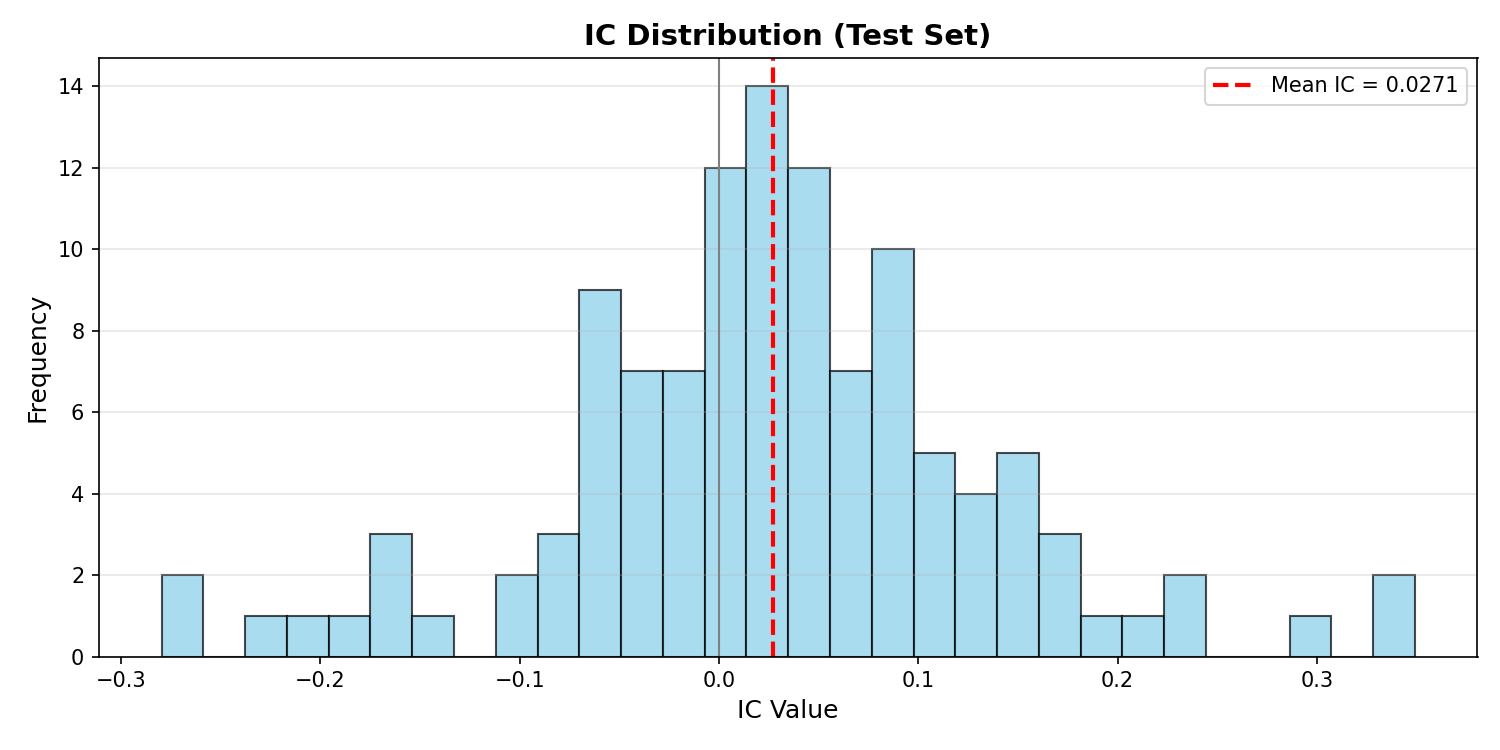
\includegraphics[width=\textwidth]{runs_gpu_static_to_20250601/static/short/gat_two_graph_no_neutral/plots/ic_distribution.png}
    \caption{GAT-TwoGraph}
  \end{subfigure}
  \hfill
  \begin{subfigure}[t]{0.47\textwidth}
    \centering
    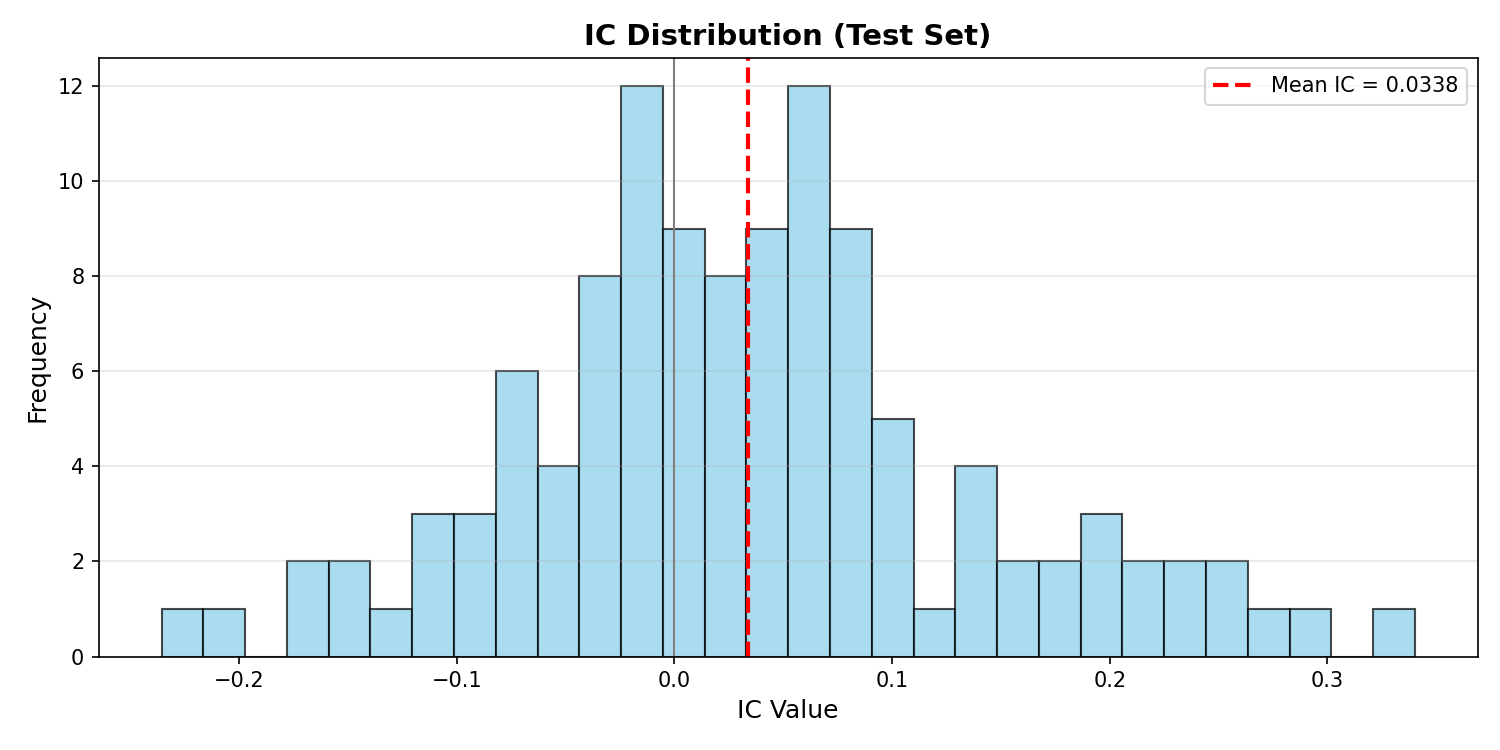
\includegraphics[width=\textwidth]{runs_gpu_static_to_20250601/static/short/dmfm_ind_neutral/plots/ic_distribution.png}
    \caption{GAT-IndNeutral}
  \end{subfigure}
  \par\vspace{0.5em}
  \hfill
  \begin{subfigure}[t]{0.47\textwidth}
    \centering
    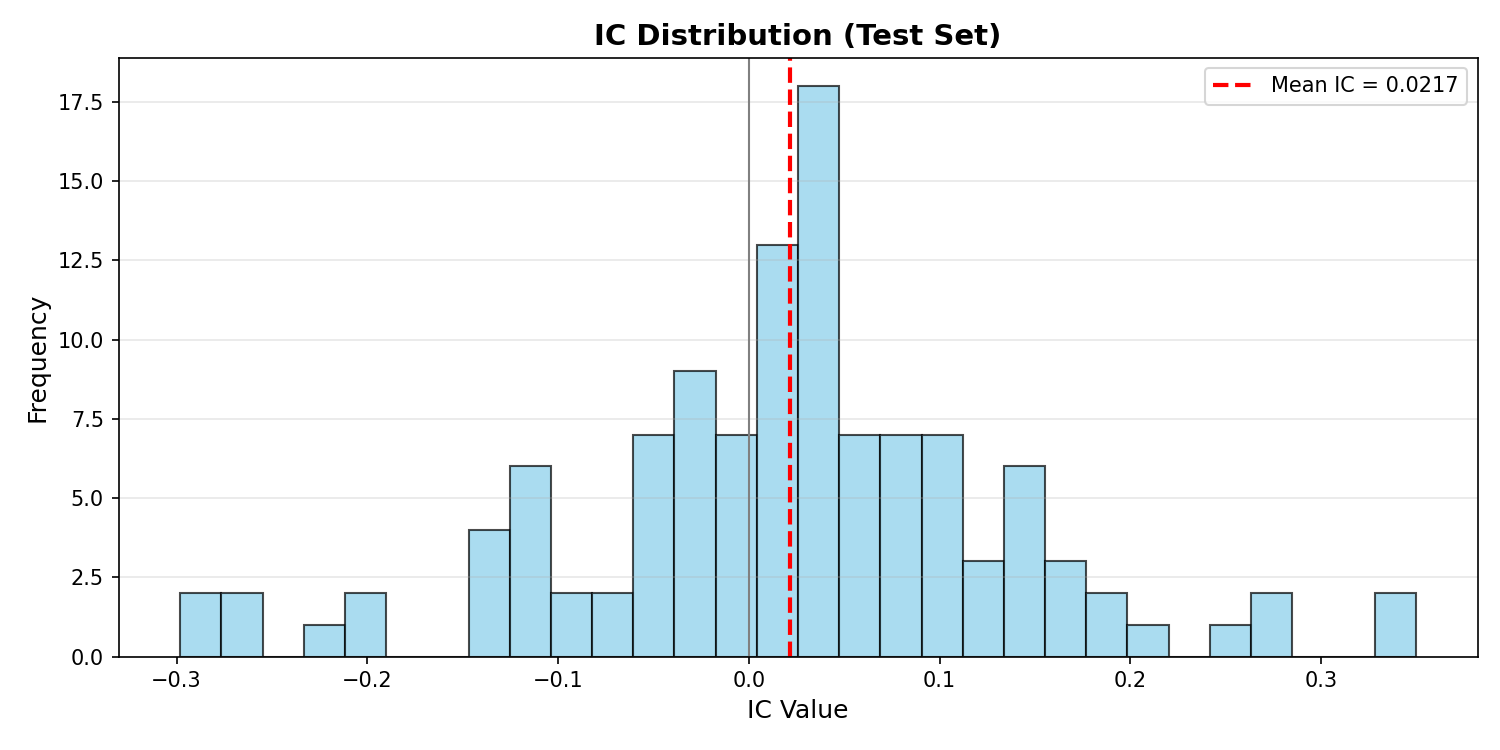
\includegraphics[width=\textwidth]{runs_gpu_static_to_20250601/static/short/dmfm_full/plots/ic_distribution.png}
    \caption{GAT-full}
  \end{subfigure}
  \hfill
  \par\vspace{0.3em}
  \caption{Short window 各模型 IC 分佈。}
  \label{fig:appendix_static_ic_distribution_short}
\end{figure}

\clearpage
\begin{figure}[H]
  \centering
  \captionsetup[subfigure]{font=small}
  \begin{subfigure}[t]{0.47\textwidth}
    \centering
    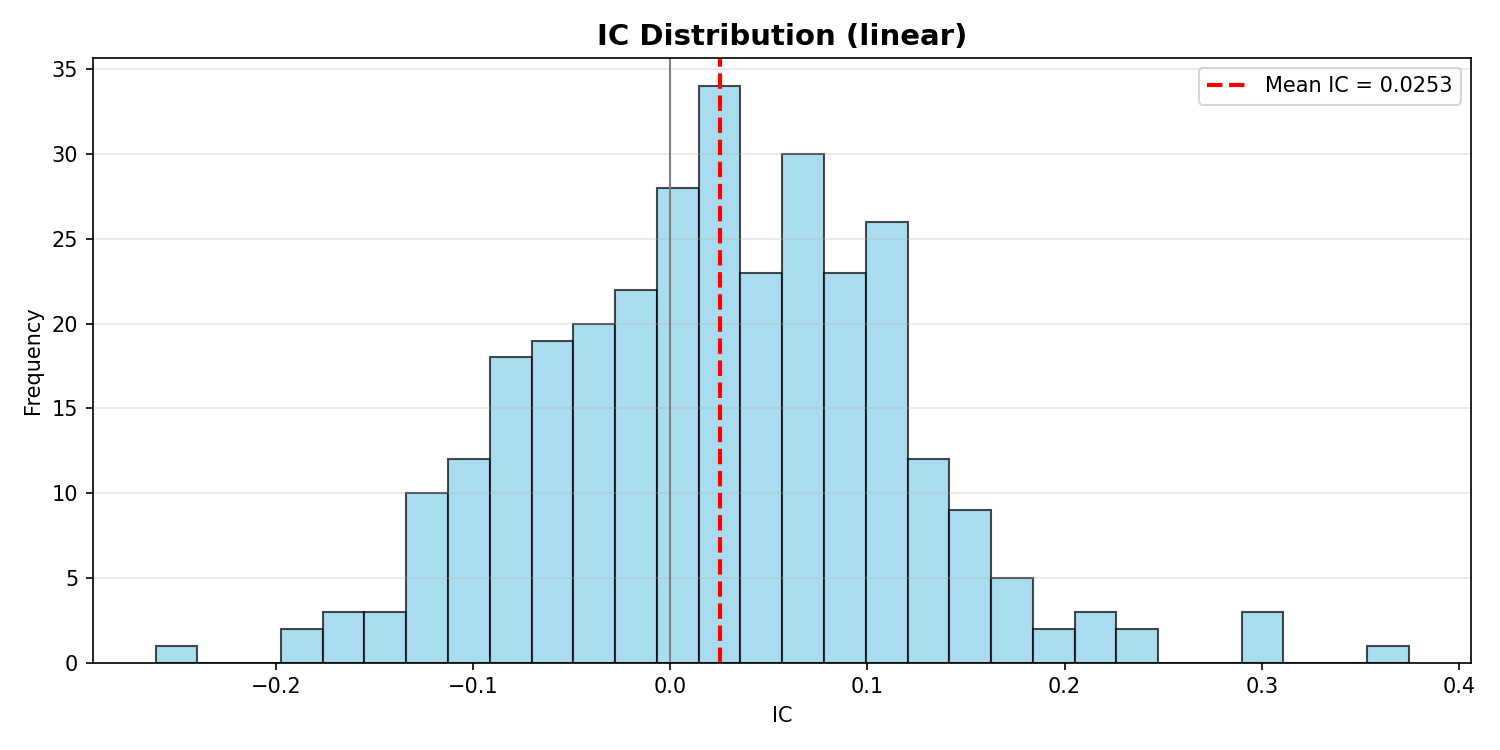
\includegraphics[width=\textwidth]{runs_gpu_static_to_20250601/static/medium/baseline_linear/plots/ic_distribution.png}
    \caption{Linear}
  \end{subfigure}
  \hfill
  \begin{subfigure}[t]{0.47\textwidth}
    \centering
    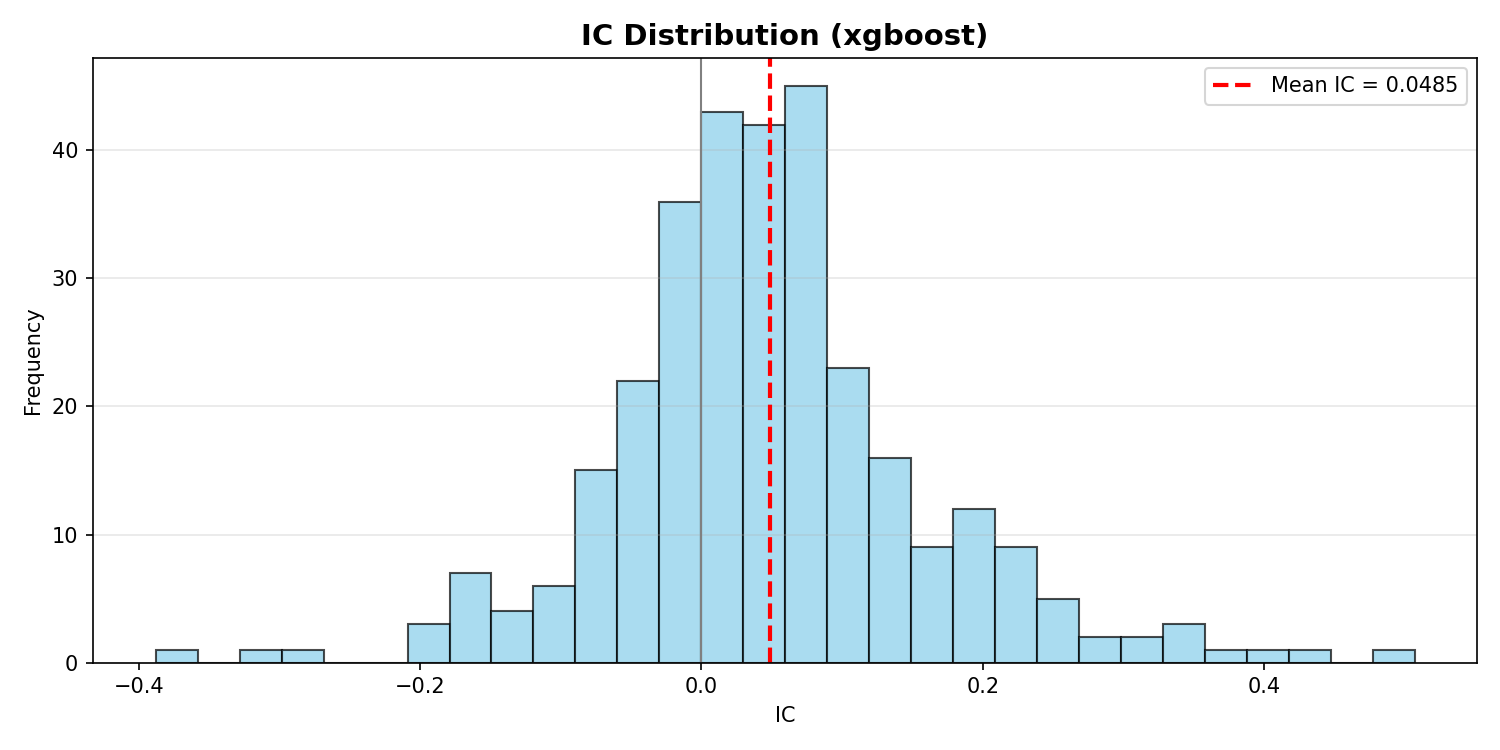
\includegraphics[width=\textwidth]{runs_gpu_static_to_20250601/static/medium/baseline_xgboost/plots/ic_distribution.png}
    \caption{XGBoost}
  \end{subfigure}
  \par\vspace{0.5em}
  \begin{subfigure}[t]{0.47\textwidth}
    \centering
    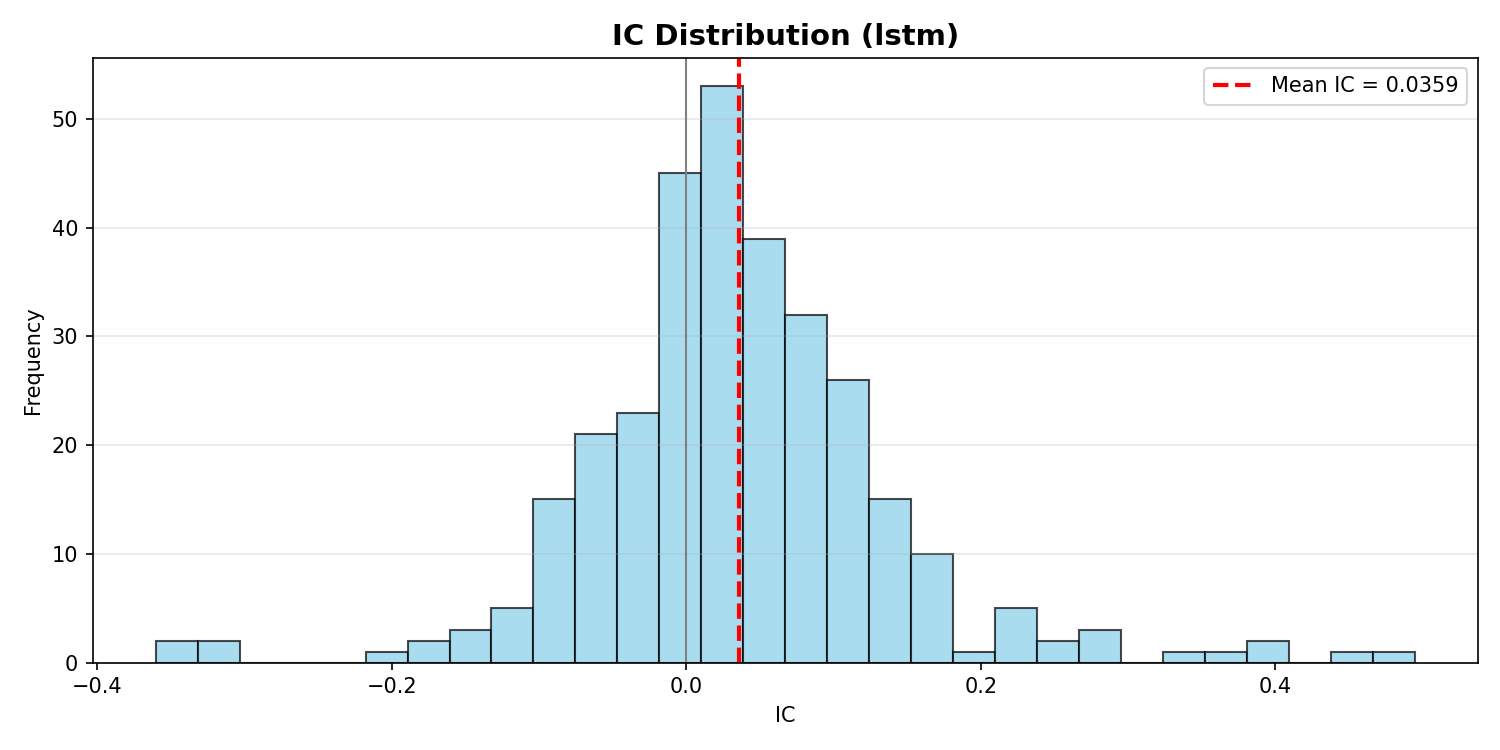
\includegraphics[width=\textwidth]{runs_gpu_static_to_20250601/static/medium/baseline_lstm/plots/ic_distribution.png}
    \caption{LSTM}
  \end{subfigure}
  \hfill
  \begin{subfigure}[t]{0.47\textwidth}
    \centering
    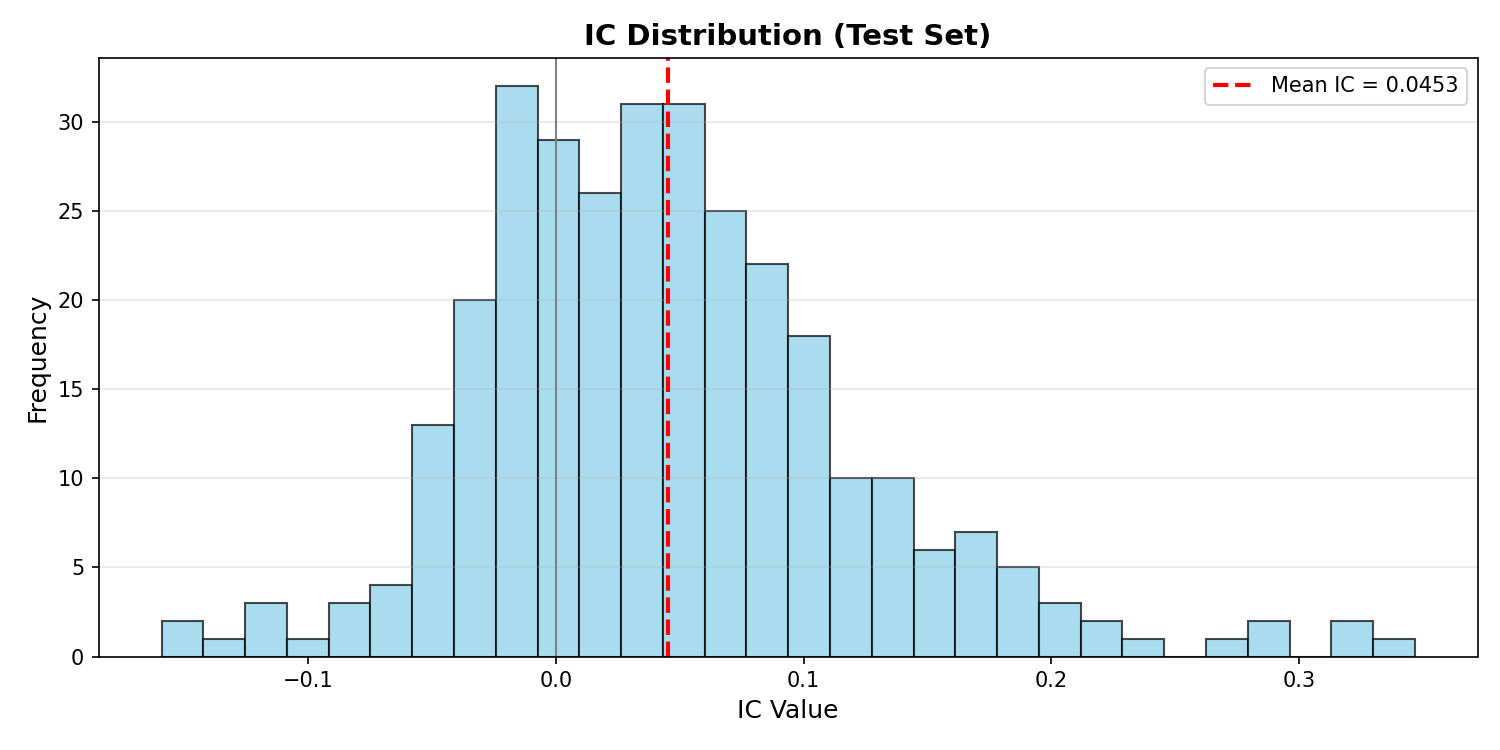
\includegraphics[width=\textwidth]{runs_gpu_static_to_20250601/static/medium/mlp/plots/ic_distribution.png}
    \caption{DNN}
  \end{subfigure}
  \par\vspace{0.5em}
  \begin{subfigure}[t]{0.47\textwidth}
    \centering
    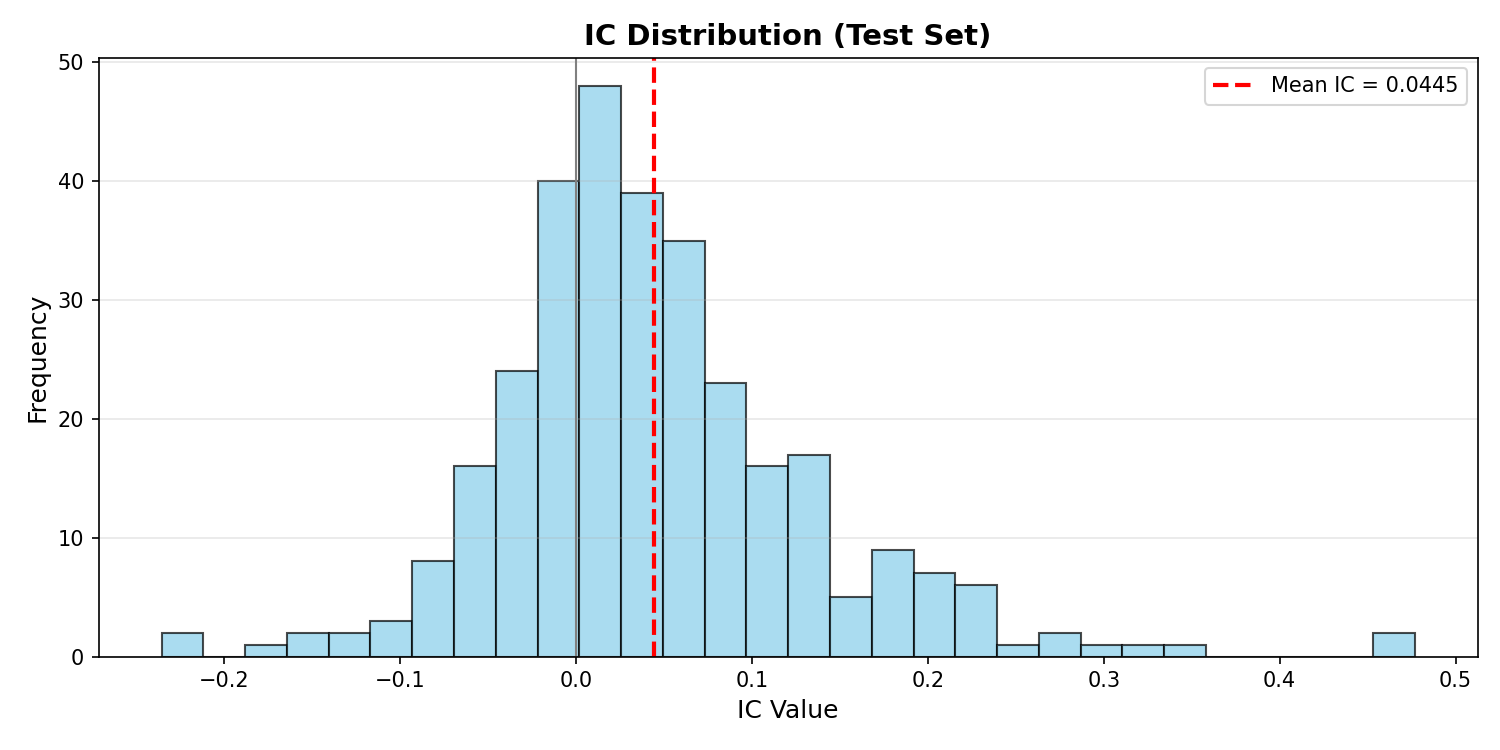
\includegraphics[width=\textwidth]{runs_gpu_static_to_20250601/static/medium/gat_industry/plots/ic_distribution.png}
    \caption{GAT-industry}
  \end{subfigure}
  \hfill
  \begin{subfigure}[t]{0.47\textwidth}
    \centering
    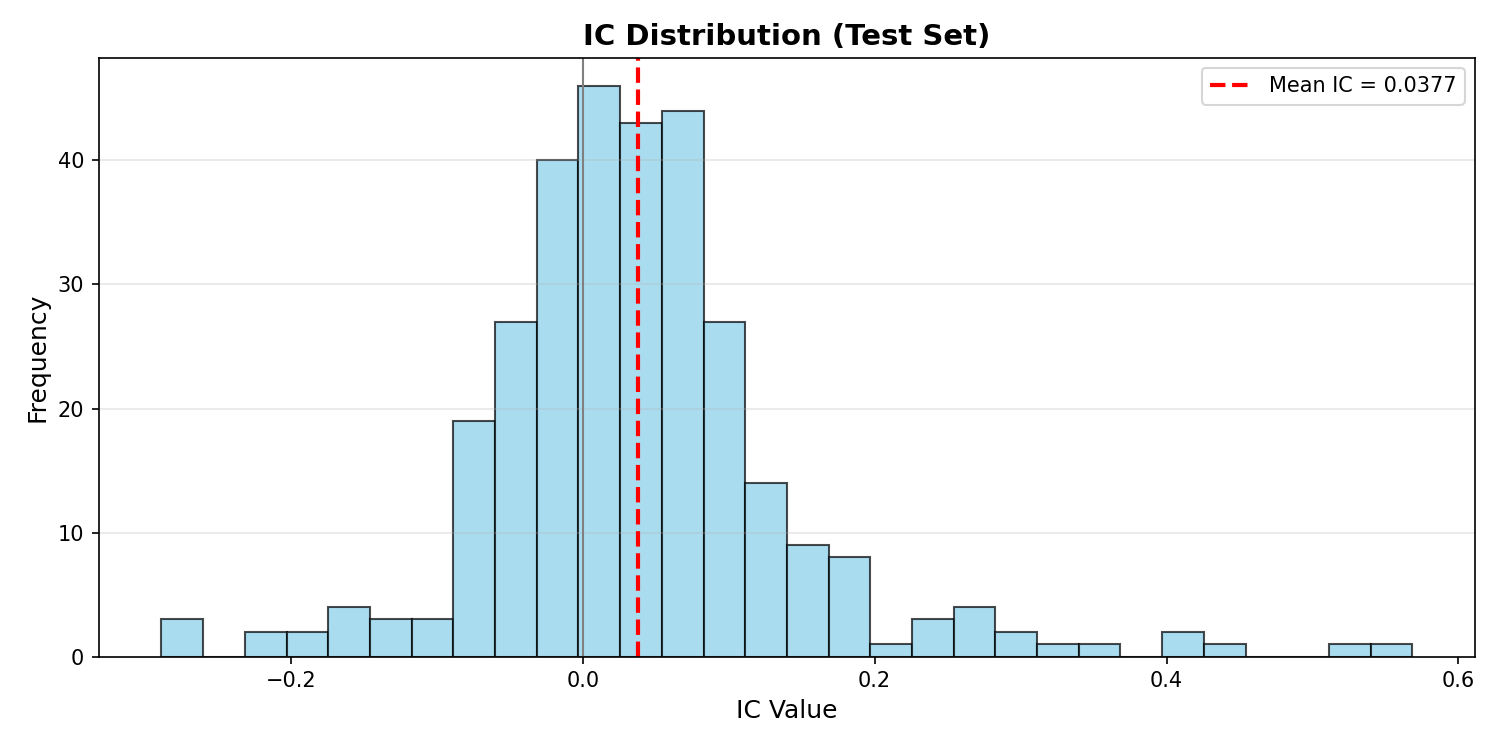
\includegraphics[width=\textwidth]{runs_gpu_static_to_20250601/static/medium/gat_universe/plots/ic_distribution.png}
    \caption{GAT-universe}
  \end{subfigure}
  \par\vspace{0.5em}
  \begin{subfigure}[t]{0.47\textwidth}
    \centering
    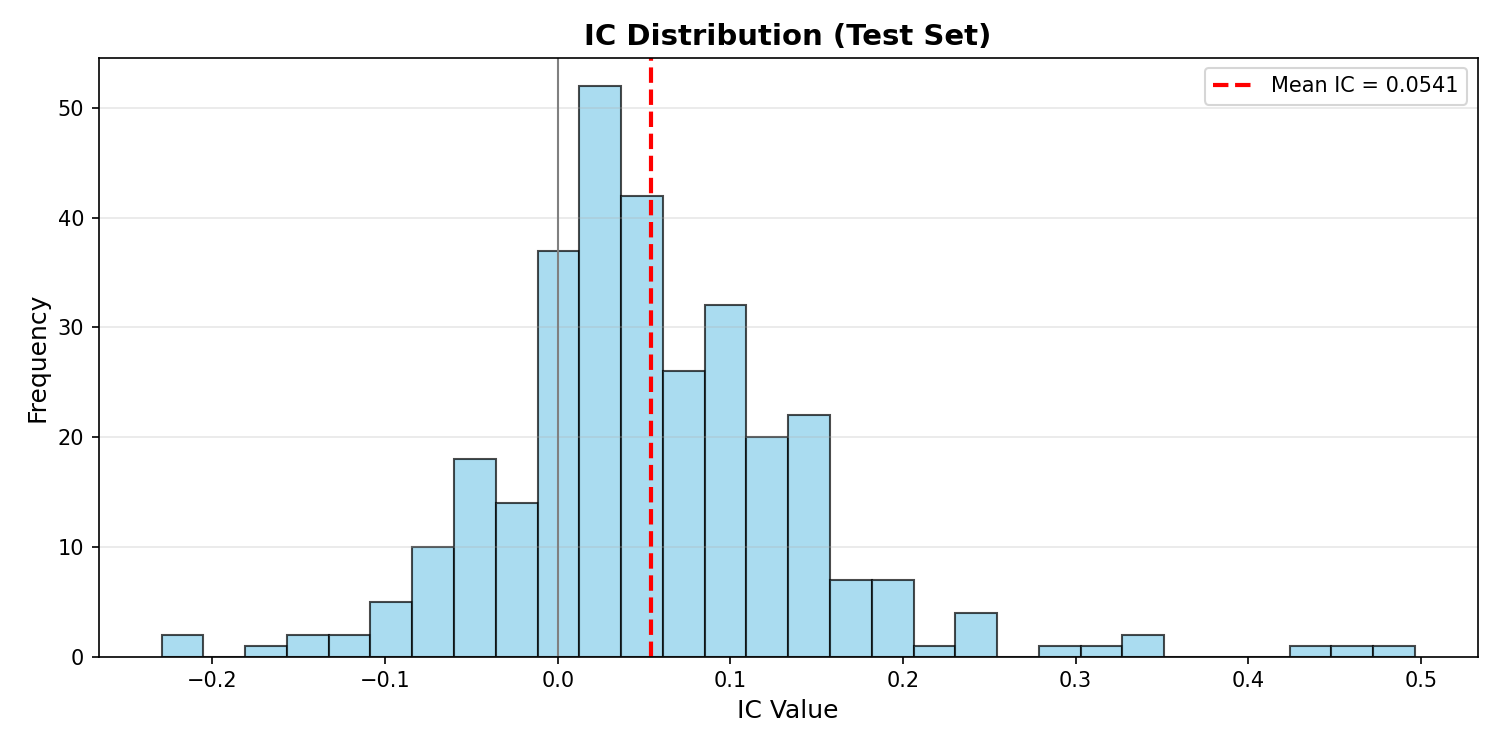
\includegraphics[width=\textwidth]{runs_gpu_static_to_20250601/static/medium/gat_two_graph_no_neutral/plots/ic_distribution.png}
    \caption{GAT-TwoGraph}
  \end{subfigure}
  \hfill
  \begin{subfigure}[t]{0.47\textwidth}
    \centering
    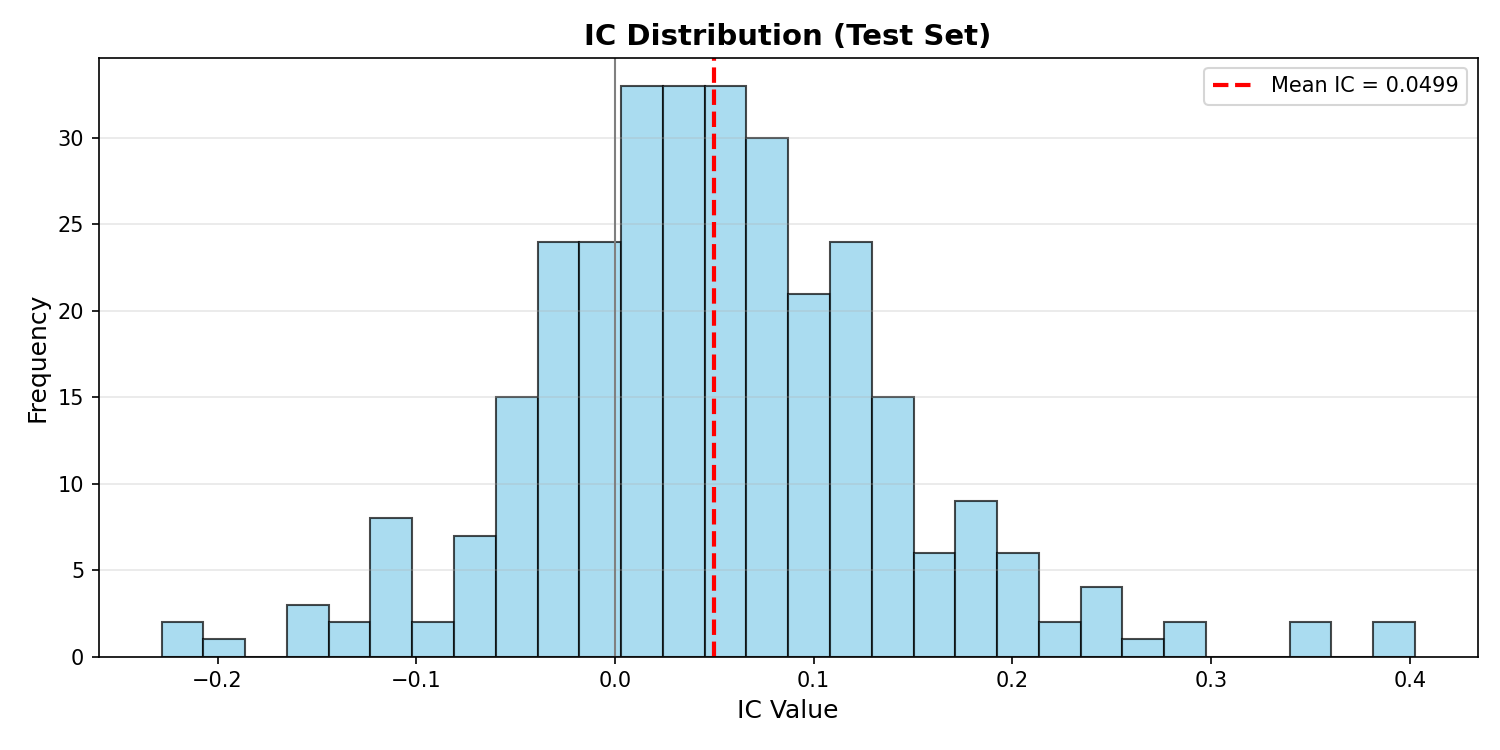
\includegraphics[width=\textwidth]{runs_gpu_static_to_20250601/static/medium/dmfm_ind_neutral/plots/ic_distribution.png}
    \caption{GAT-IndNeutral}
  \end{subfigure}
  \par\vspace{0.5em}
  \hfill
  \begin{subfigure}[t]{0.47\textwidth}
    \centering
    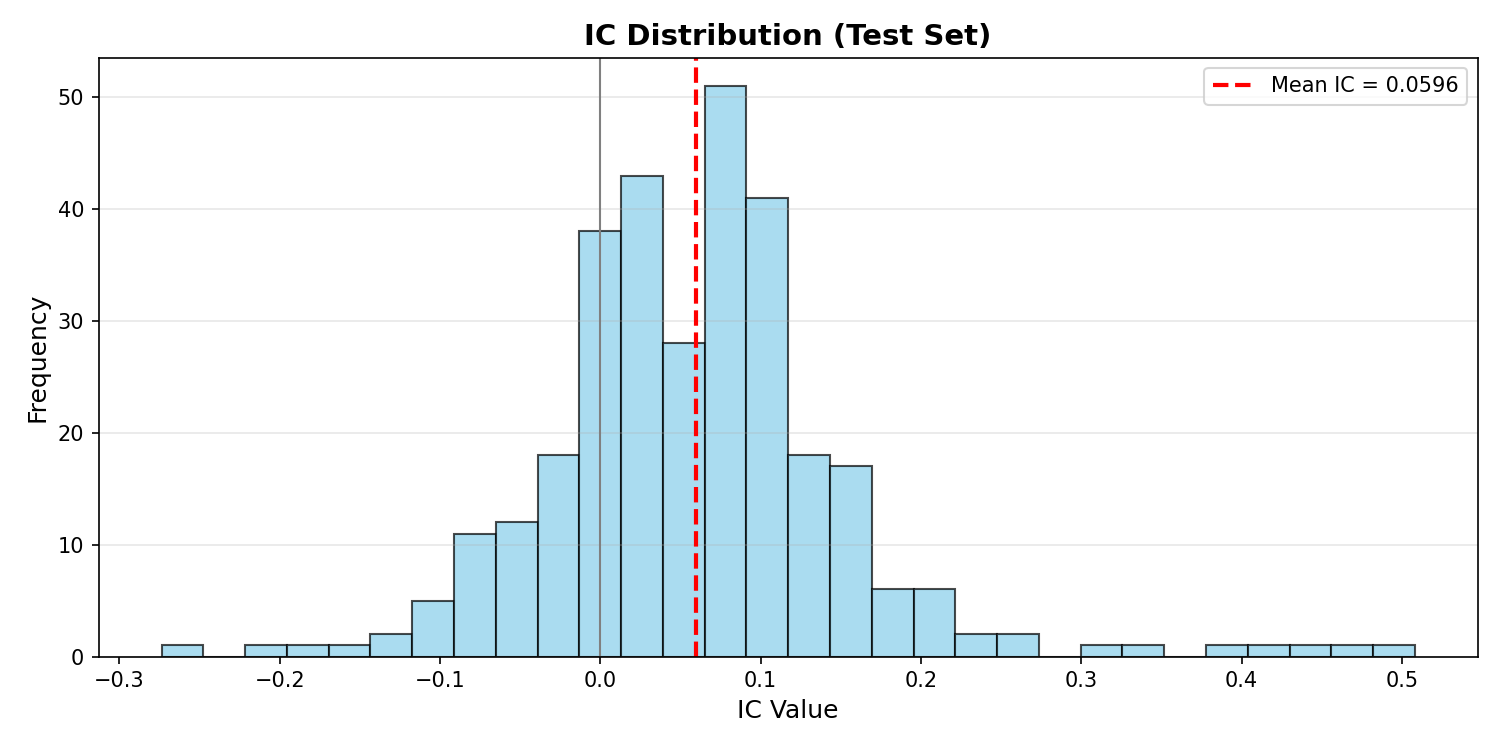
\includegraphics[width=\textwidth]{runs_gpu_static_to_20250601/static/medium/dmfm_full/plots/ic_distribution.png}
    \caption{GAT-full}
  \end{subfigure}
  \hfill
  \par\vspace{0.3em}
  \caption{Medium window 各模型 IC 分佈。}
  \label{fig:appendix_static_ic_distribution_medium}
\end{figure}

\clearpage
\begin{figure}[H]
  \centering
  \captionsetup[subfigure]{font=small}
  \begin{subfigure}[t]{0.47\textwidth}
    \centering
    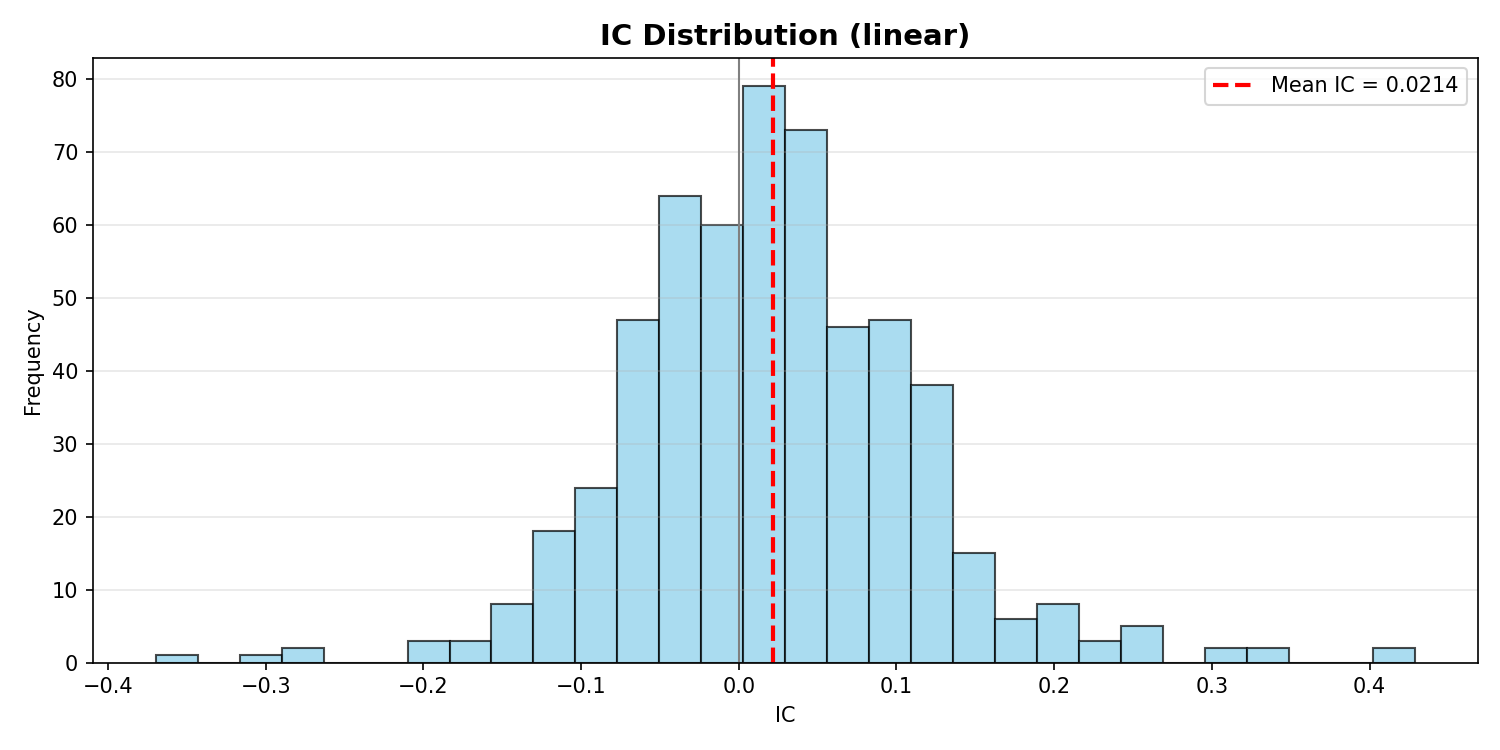
\includegraphics[width=\textwidth]{runs_gpu_static_to_20250601/static/long/baseline_linear/plots/ic_distribution.png}
    \caption{Linear}
  \end{subfigure}
  \hfill
  \begin{subfigure}[t]{0.47\textwidth}
    \centering
    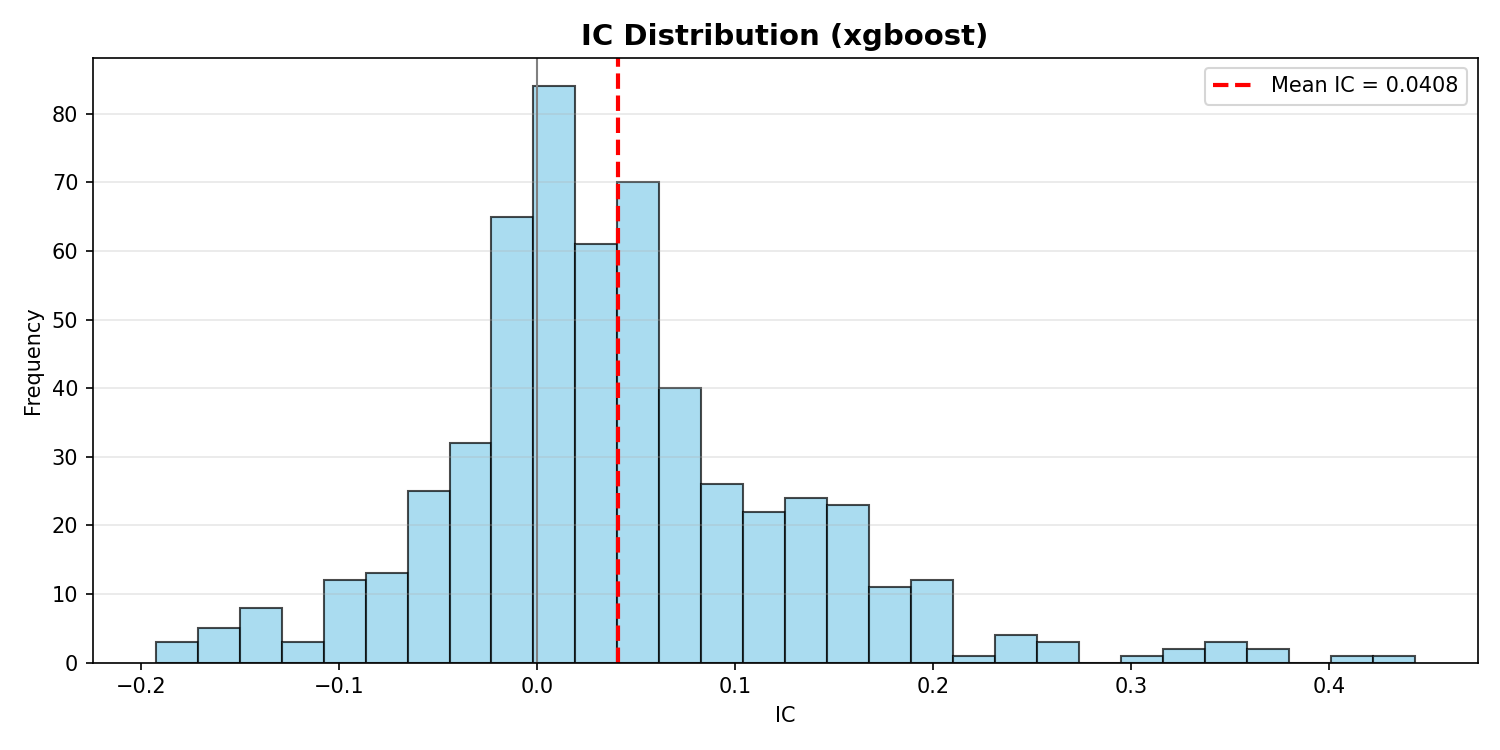
\includegraphics[width=\textwidth]{runs_gpu_static_to_20250601/static/long/baseline_xgboost/plots/ic_distribution.png}
    \caption{XGBoost}
  \end{subfigure}
  \par\vspace{0.5em}
  \begin{subfigure}[t]{0.47\textwidth}
    \centering
    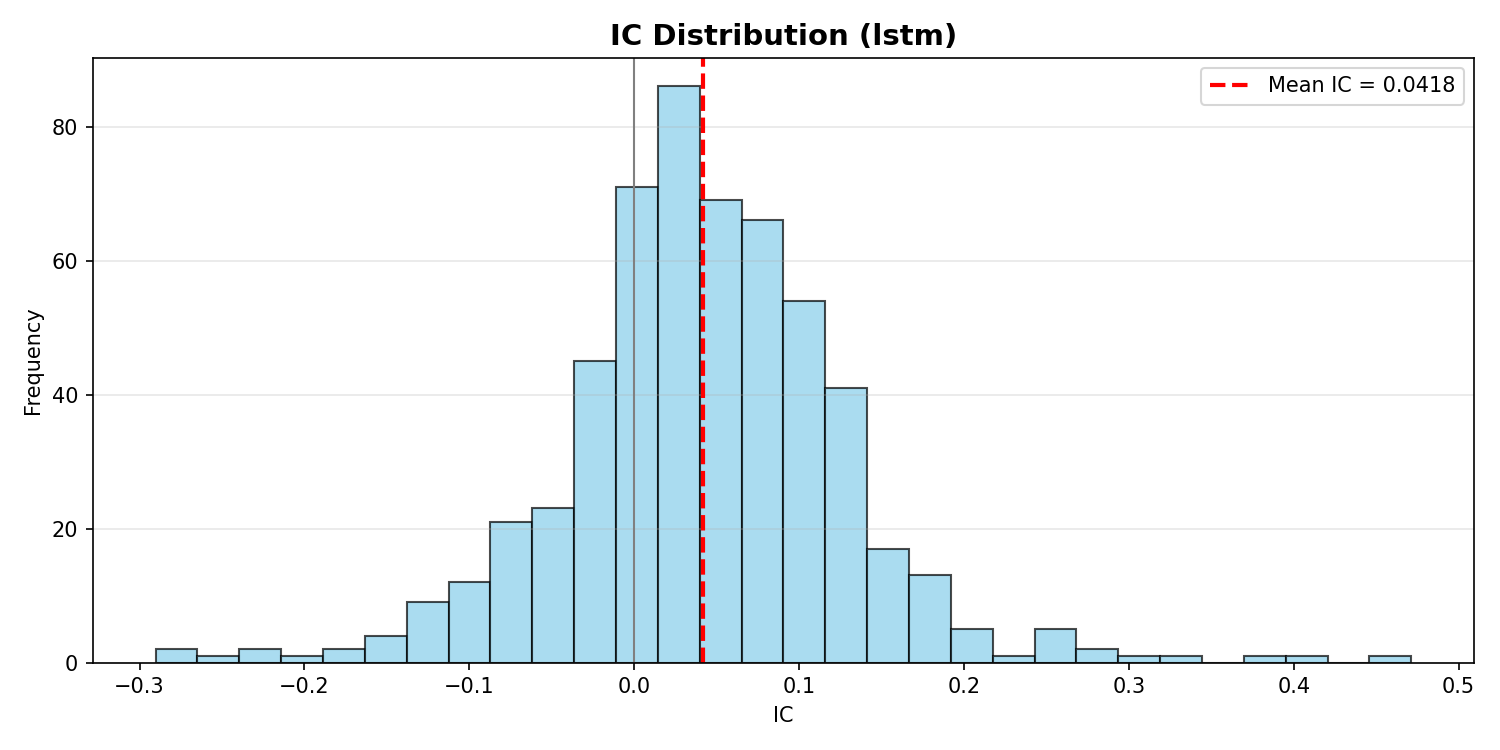
\includegraphics[width=\textwidth]{runs_gpu_static_to_20250601/static/long/baseline_lstm/plots/ic_distribution.png}
    \caption{LSTM}
  \end{subfigure}
  \hfill
  \begin{subfigure}[t]{0.47\textwidth}
    \centering
    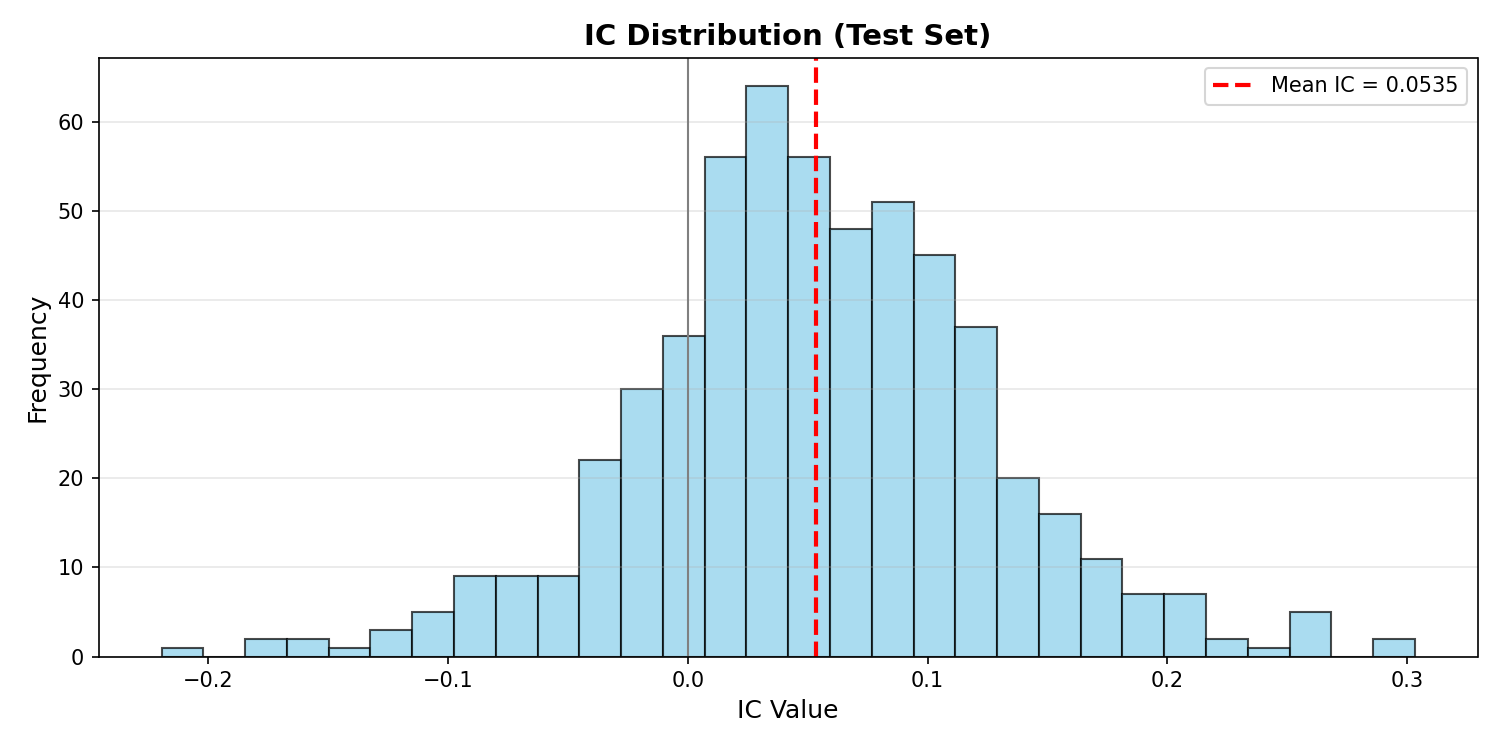
\includegraphics[width=\textwidth]{runs_gpu_static_to_20250601/static/long/mlp/plots/ic_distribution.png}
    \caption{DNN}
  \end{subfigure}
  \par\vspace{0.5em}
  \begin{subfigure}[t]{0.47\textwidth}
    \centering
    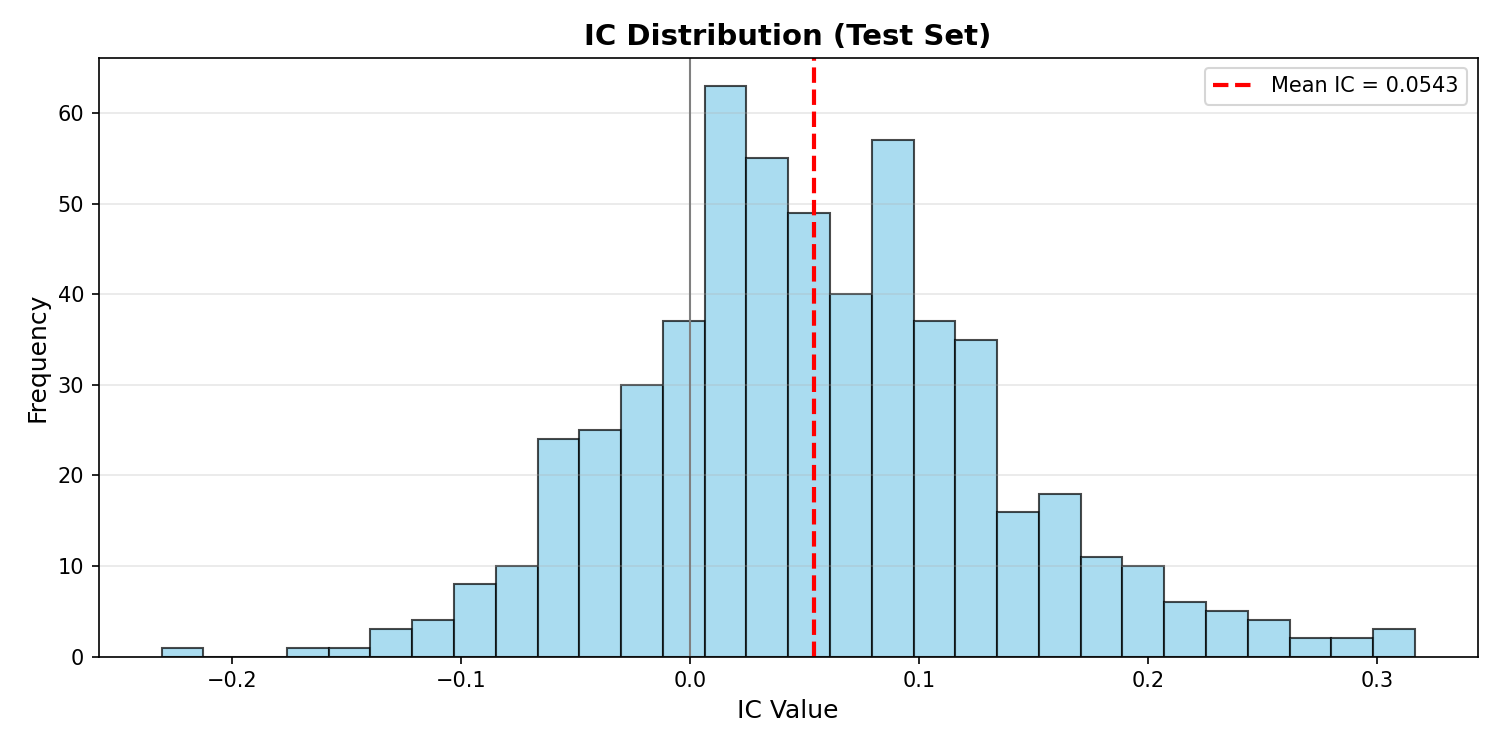
\includegraphics[width=\textwidth]{runs_gpu_static_to_20250601/static/long/gat_industry/plots/ic_distribution.png}
    \caption{GAT-industry}
  \end{subfigure}
  \hfill
  \begin{subfigure}[t]{0.47\textwidth}
    \centering
    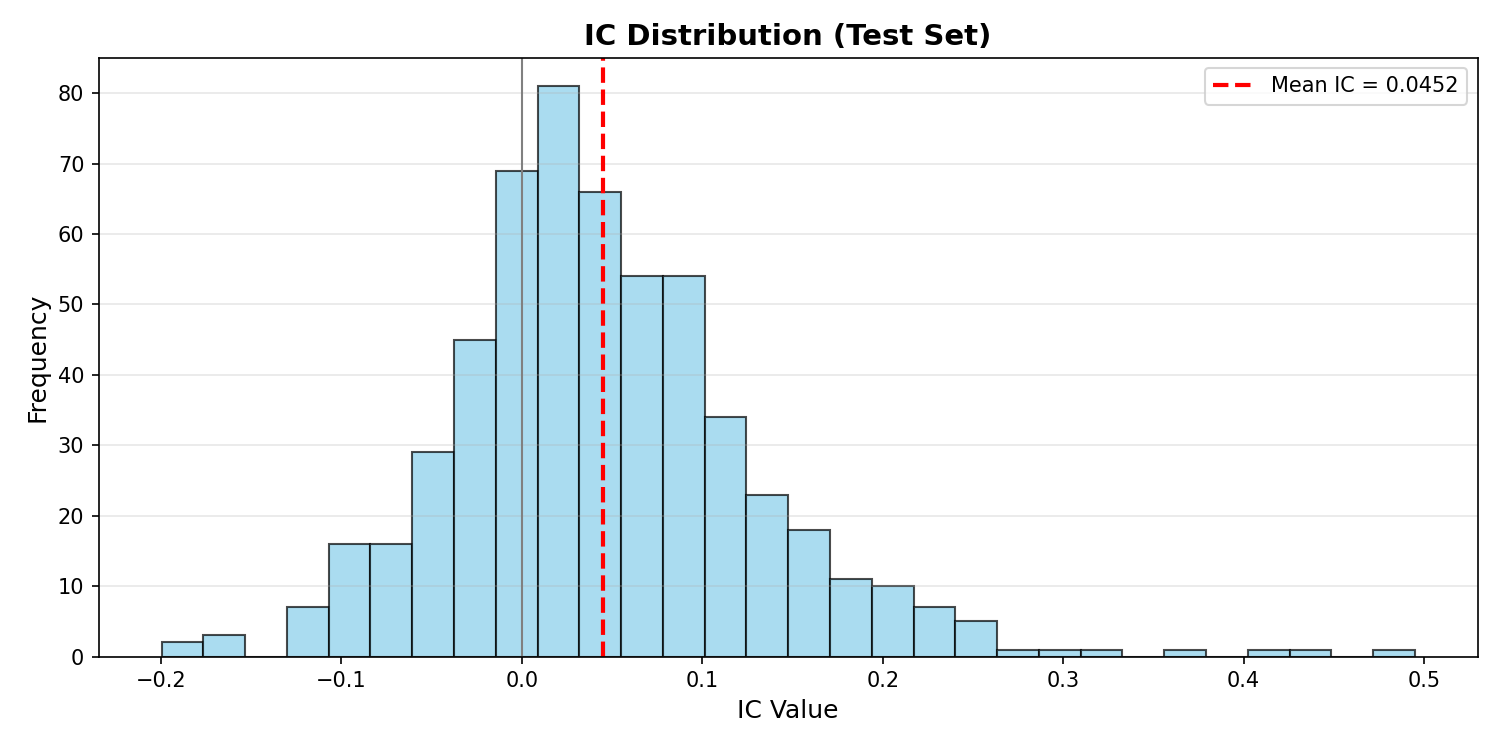
\includegraphics[width=\textwidth]{runs_gpu_static_to_20250601/static/long/gat_universe/plots/ic_distribution.png}
    \caption{GAT-universe}
  \end{subfigure}
  \par\vspace{0.5em}
  \begin{subfigure}[t]{0.47\textwidth}
    \centering
    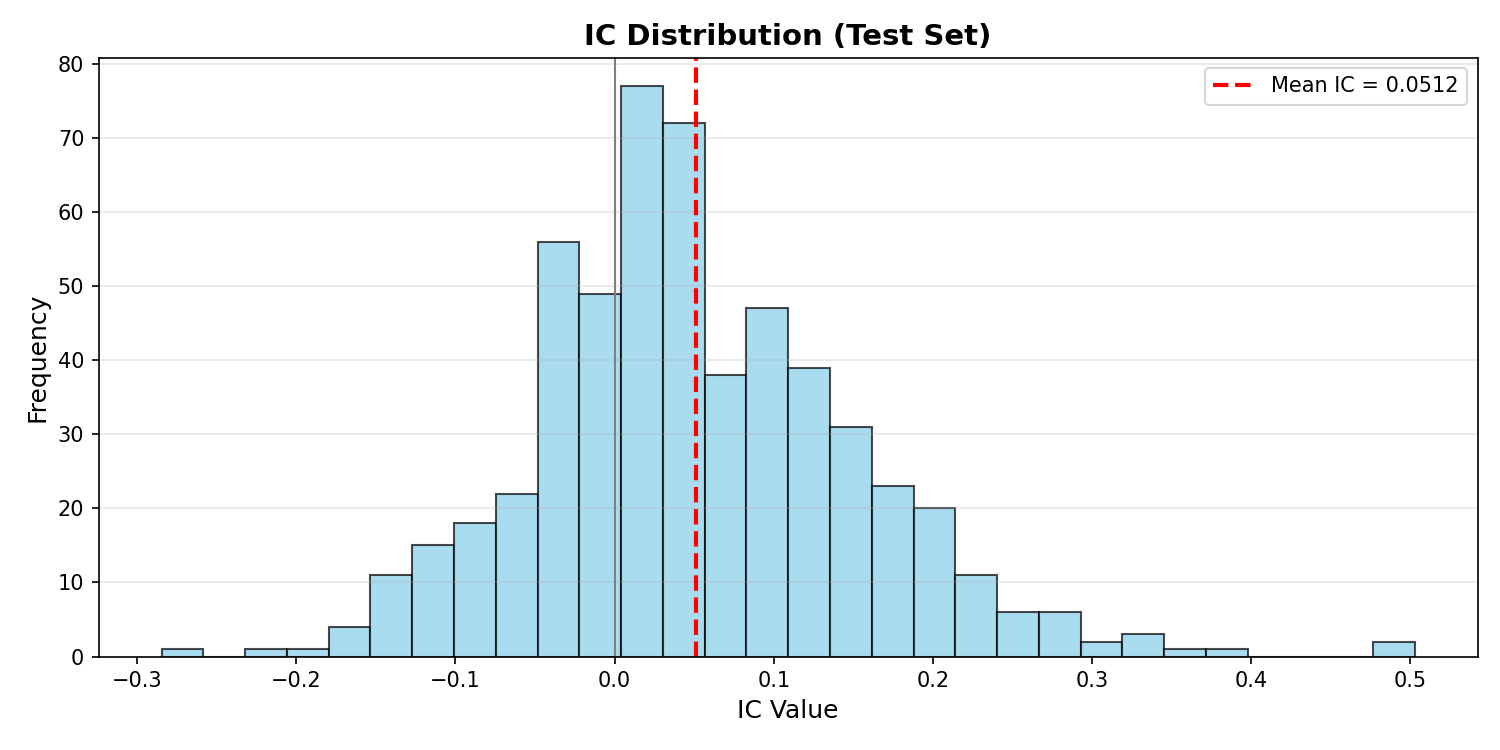
\includegraphics[width=\textwidth]{runs_gpu_static_to_20250601/static/long/gat_two_graph_no_neutral/plots/ic_distribution.png}
    \caption{GAT-TwoGraph}
  \end{subfigure}
  \hfill
  \begin{subfigure}[t]{0.47\textwidth}
    \centering
    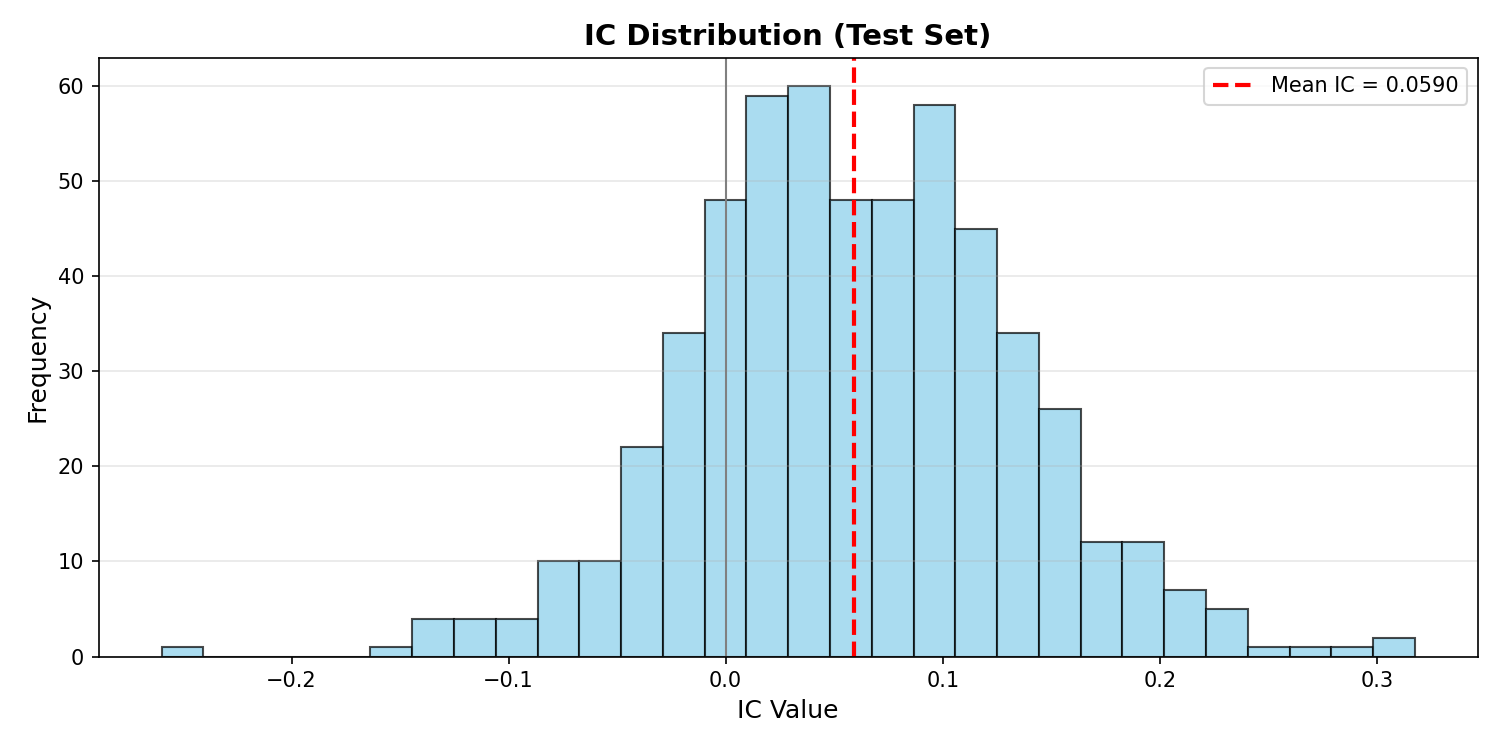
\includegraphics[width=\textwidth]{runs_gpu_static_to_20250601/static/long/dmfm_ind_neutral/plots/ic_distribution.png}
    \caption{GAT-IndNeutral}
  \end{subfigure}
  \par\vspace{0.5em}
  \hfill
  \begin{subfigure}[t]{0.47\textwidth}
    \centering
    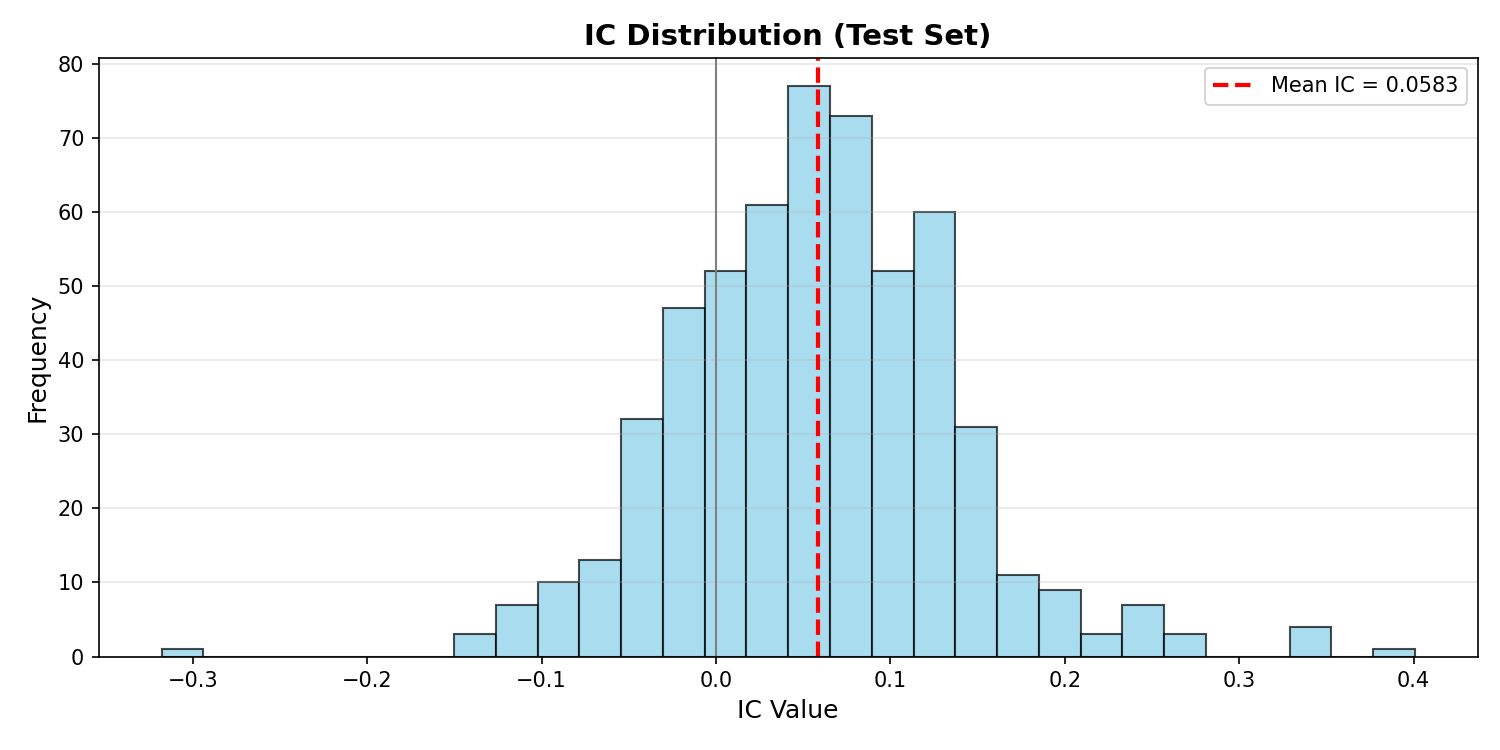
\includegraphics[width=\textwidth]{runs_gpu_static_to_20250601/static/long/dmfm_full/plots/ic_distribution.png}
    \caption{GAT-full}
  \end{subfigure}
  \hfill
  \par\vspace{0.3em}
  \caption{Long window 各模型 IC 分佈。}
  \label{fig:appendix_static_ic_distribution_long}
\end{figure}
